% Autor: Daniel Núñez-Agurto
% 1ra versión: 28/10/2022
% ültima actualización: 02/05/2023
% @COPYLEFT


%https://www.overleaf.com/latex/templates/template-and-sample-for-authoring-apa7-manuscripts/pvhtwcrvcmsp

%+-+-+-+-++-+-+-+-+-+-+-+-+-++-+-+-+-+-+-+-+-+-+-+-+-+-+-+-+-+-++-+-+-+-+-+-+-+-+-+
% Preámbulo
%\documentclass[stu, 11pt, letterpaper, donotrepeattitle, floatsintext, natbib]{apa7}

\documentclass[letterpaper, 12pt, journal, oneside, onecolumn]{IEEEtran}

\usepackage[utf8]{inputenc}
\usepackage[spanish]{babel}
\usepackage{csquotes}
\usepackage[backend=biber,style=ieee]{biblatex}
\usepackage{geometry}
\usepackage[table,xcdraw]{xcolor}
\usepackage{colortbl}
\usepackage{float}
\usepackage{makecell}
\usepackage{tcolorbox}
\usepackage{times}
\usepackage{titlesec}
\usepackage{setspace}
\usepackage{multicol}
\usepackage[table]{xcolor}
\usepackage{hyperref}
\usepackage{tikz,xcolor,hyperref}
\usepackage{pdflscape}
\usepackage{comment}
\usepackage{marvosym}
\usepackage{graphicx}
\usepackage{float}
\usepackage{indentfirst}
\usepackage{longtable}
\usepackage{listings}
\usepackage{algorithm}
\usepackage{algpseudocode}
\usepackage{amsmath}
\usepackage{pdfpages}
\usepackage{caption}
\usepackage[normalem]{ulem}
\usepackage{multirow}
\usepackage{url}
\usepackage{enumitem}
\usepackage[utf8]{inputenc}
\usepackage{tabularx}
\usepackage{booktabs}
\usepackage{upquote}
\usepackage{fancyhdr}  % PAQUETE NECESARIO para controlar numeración de páginas
\usepackage{comment}
\usepackage{marvosym}
\usepackage{graphicx}
\usepackage{float}
\usepackage{indentfirst}
\usepackage{longtable}
\usepackage{listings}
\usepackage{algorithm}
\usepackage{algpseudocode}
\usepackage{amsmath}
\usepackage{pdfpages}
%fuente
%\usepackage{fontspec}
%\setmainfont{Calibri}
%\usepackage{caption}
\usepackage[normalem]{ulem}
\usepackage{multirow}
\usepackage{url}
%\usepackage{hyperref}
\usepackage{enumitem}
\usepackage{etoolbox}
%---titles
\usepackage{titlesec}
\usepackage{titletoc}

\definecolor{FF6666}{HTML}{FF6666}
\definecolor{FFCC66}{HTML}{FFCC66}
\definecolor{FFEB99}{HTML}{FFEB99}
\definecolor{FF9999}{HTML}{FF9999}
\definecolor{FFFF99}{HTML}{FFFF99}
\definecolor{CCFFCC}{HTML}{CCFFCC}




\geometry{
    left=2.5cm,
    right=2.5cm,
    top=2.5cm,
    bottom=2.5cm
}


\addbibresource{bibliografia/referencias.bib}

\renewcommand{\baselinestretch}{1.5}
\parskip=6pt
\setlength{\parindent}{0.5in}


\captionsetup[figure]{justification=centering, singlelinecheck=false, font=footnotesize, format=plain, labelsep=period, name=Fig.}

\captionsetup[table]{name=Tabla, labelfont=sc, labelsep=newline, justification=centering, font=footnotesize, singlelinecheck=false, format=plain, skip=1ex}
%\captionsetup[table]{name=Tabla, labelsep=period, justification=centering, font=footnotesize, singlelinecheck=false, format=plain, skip=1ex}

\renewcommand{\textspanish}{}


\titleformat{\chapter}[block]
{\large\filcenter}
{\thechapter.}
{5pt}
{\MakeUppercase}
{}
\titlespacing{\chapter}{0pt}{0pt}{*3}
\titlecontents{chapter}
[0pt]                                               
{}
{\contentsmargin{0pt}\thecontentslabel.\enspace\uppercase}
{\contentsmargin{0pt}\uppercase}                        
{\titlerule*[.7pc]{.}\contentspage}  
\renewcommand{\thesubsection}{\Alph{subsection}}
\renewcommand{\thesubsubsection}{\arabic{subsubsection}}
\DeclareNameAlias{sortname}{family-given}

%-----------------------------------------------------------------------------------------


% ========================================
% CONFIGURACIÓN DE NUMERACIÓN DE PÁGINAS
% ========================================

% OPCIÓN 1: NUMERACIÓN EN ESQUINA SUPERIOR DERECHA (ACTUAL)
\setlength{\headheight}{14.5pt} % Altura del área del encabezado
\pagestyle{fancy}               % Activa el estilo de página personalizado
\fancyhf{}                     % Limpia todos los encabezados y pies de página
\fancyhead[R]{\thepage}        % ← LÍNEA PRINCIPAL: Número en esquina superior derecha
\renewcommand{\headrulewidth}{0pt} % Sin línea horizontal en el encabezado

% Configuración para páginas especiales (inicio de secciones, capítulos)
\fancypagestyle{plain}{
    \fancyhf{}                 % Limpia encabezados y pies
    \fancyhead[R]{\thepage}    % ← LÍNEA SECUNDARIA: Número en esquina superior derecha para páginas especiales
    \renewcommand{\headrulewidth}{0pt} % Sin línea horizontal
}
% ========================================
% OPCIÓN 2: NUMERACIÓN EN PARTE INFERIOR CENTRAL (CÓDIGO ALTERNATIVO)
% ========================================
% Para cambiar a numeración en la parte inferior central, 
% COMENTA las líneas de arriba y DESCOMENTA las líneas de abajo:

%\setlength{\headheight}{14.5pt} % Mantener altura del encabezado
%\pagestyle{fancy}               % Activa el estilo personalizado
%\fancyhf{}                     % Limpia todos los encabezados y pies
%\fancyfoot[C]{\thepage}        % ← NÚMERO EN PARTE INFERIOR CENTRAL
%\renewcommand{\headrulewidth}{0pt}  % Sin línea en encabezado
%\renewcommand{\footrulewidth}{0pt}  % Sin línea en pie de página

% % Configuración para páginas especiales con numeración inferior central
%\fancypagestyle{plain}{
%     \fancyhf{}                 % Limpia encabezados y pies
%     \fancyfoot[C]{\thepage}    % ← NÚMERO EN PARTE INFERIOR CENTRAL para páginas especiales
%     \renewcommand{\headrulewidth}{0pt} % Sin línea en encabezado
%     \renewcommand{\footrulewidth}{0pt} % Sin línea en pie de página
%}

% ========================================
% OTRAS OPCIONES DE POSICIÓN (EJEMPLOS):
% ========================================
% \fancyhead[L]{\thepage}  % Superior izquierda
% \fancyhead[C]{\thepage}  % Superior centro
% \fancyhead[R]{\thepage}  % Superior derecha (actual)
% \fancyfoot[L]{\thepage}  % Inferior izquierda
% \fancyfoot[C]{\thepage}  % Inferior centro
% \fancyfoot[R]{\thepage}  % Inferior derecha

\begin{document}
% Configuración de numeración desde el inicio


%Se reemplaza Tabla Nro. por Lugar de Cuadro Nro.
\renewcommand{\tablename}{Tabla}

% Portada de la tesis (página 1)
\thispagestyle{plain}
\pagestyle{plain}

\begin{figure}[t]
	\centering
	
\includegraphics[scale=0.8]{figuras/logo.png}
\end{figure}

\vspace{2cm}

\begin{center}
\textbf{PROYECTO DE TITULACIÓN}
\vspace{2cm}

Carrera de Ingeniería de Tecnologías de la Información
\vspace{2cm}

\textbf{Diseñar e implementar un sistema basado en blockchain para garantizar la integridad, trazabilidad y autenticidad de los logs de seguridad.}
\vspace{2cm}

\textbf{Autor: } Faz Intriago, Raúl Enrique
\vspace{2cm}

\textbf{Tutor: } Ing. Núñez Agurto, Alberto Daniel, PhD.
\vspace{4cm}
\begin{flushright}
Santo Domingo de los Tsáchilas, 04 de agosto del 2025
\end{flushright}
\end{center}
\thispagestyle{empty}
\newpage

% Reporte de verificación de plagio del software antiplagio 
%\phantomsection
%\addcontentsline{toc}{section}{Reporte de Verificación de Plagio}

%\thispagestyle{fancy}
\begin{center}
\textbf{Reporte de verificación de contenido}
\end{center}
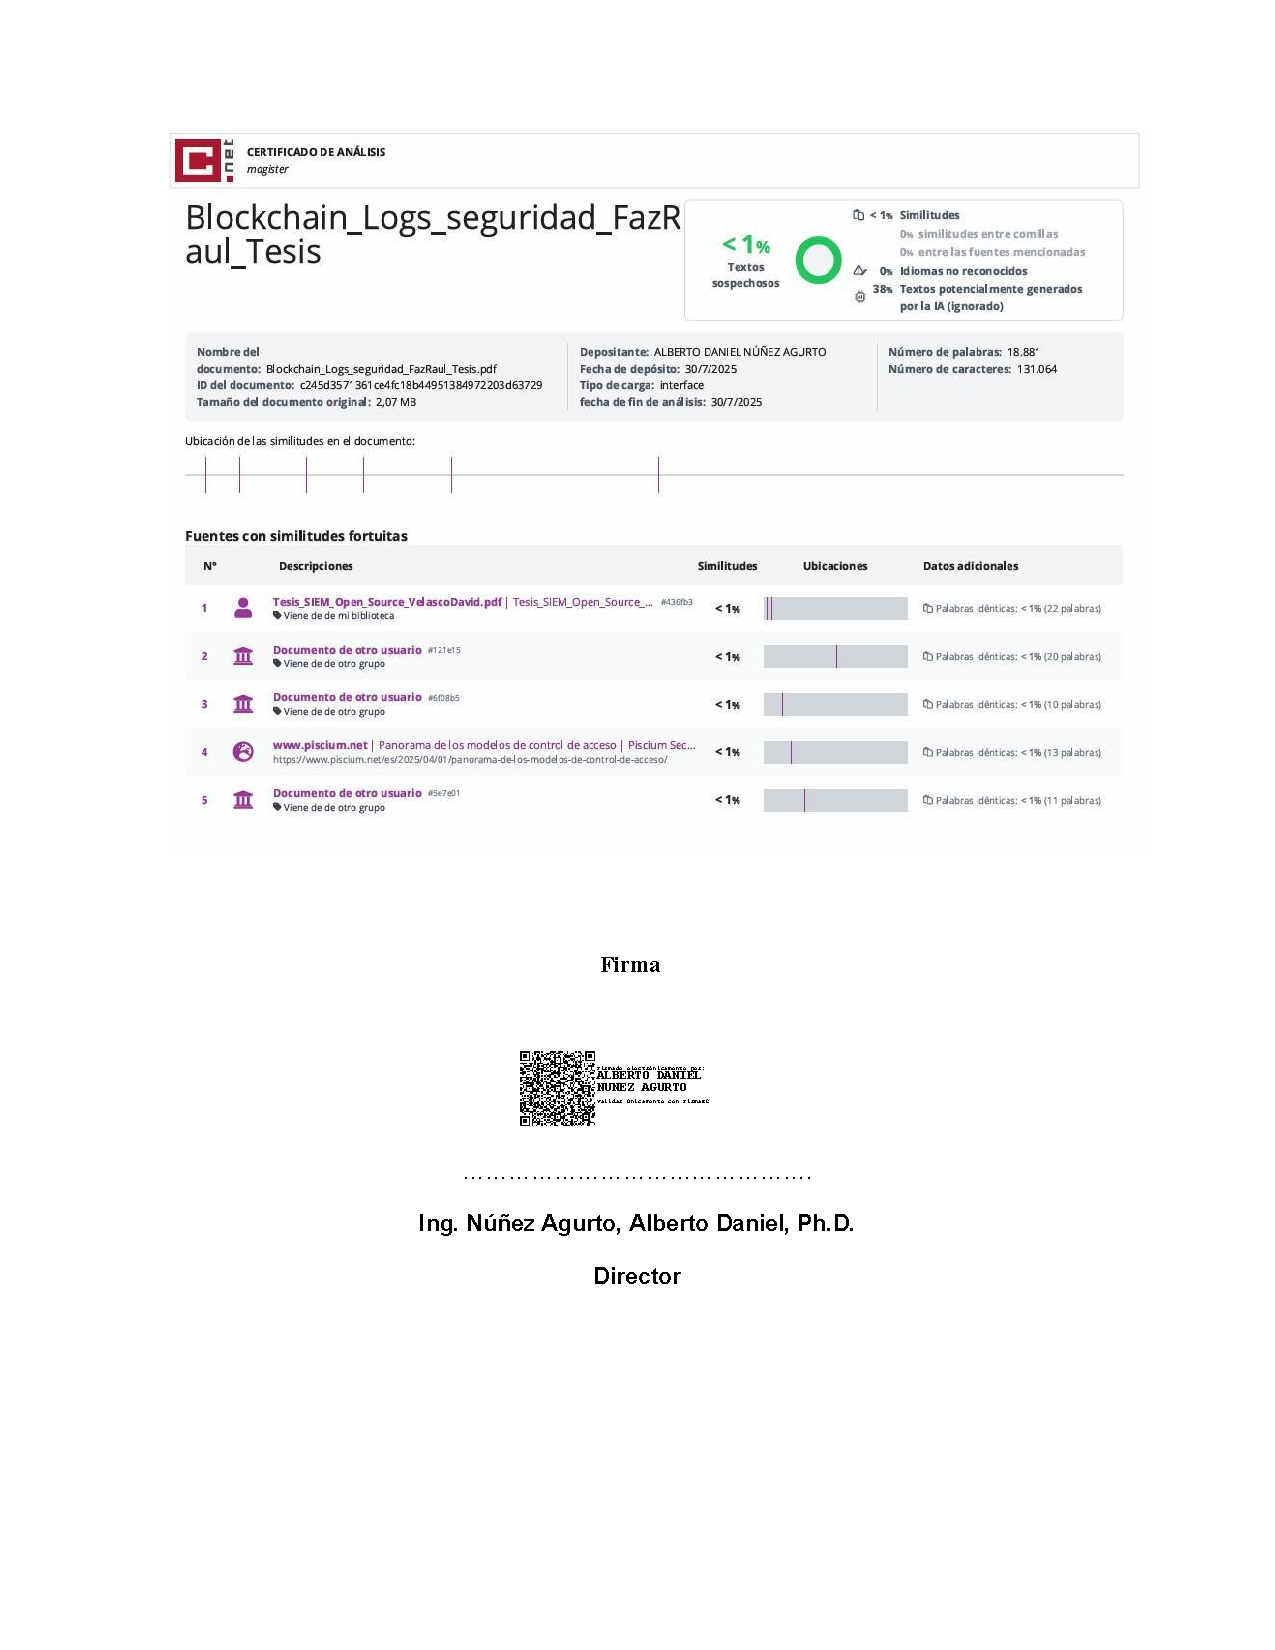
\includegraphics[width=\textwidth,height=0.9\textheight,keepaspectratio]{figuras/RF_ReportePlagio.pdf}
\thispagestyle{empty}
\newpage

% Certificación de trabajo de titulación (Firma tutor/ Director de tesis)
%\phantomsection
%\addcontentsline{toc}{section}{Certificación}

\includepdf[pages=1,fitpaper=true,pagecommand={\thispagestyle{empty}}]{figuras/RF_CertificadoDirectorTesis.pdf}
\newpage

% Responsabilidad de autoria firmada por el tesista
%\phantomsection
%\addcontentsline{toc}{section}{Responsabilidad de Autoría}
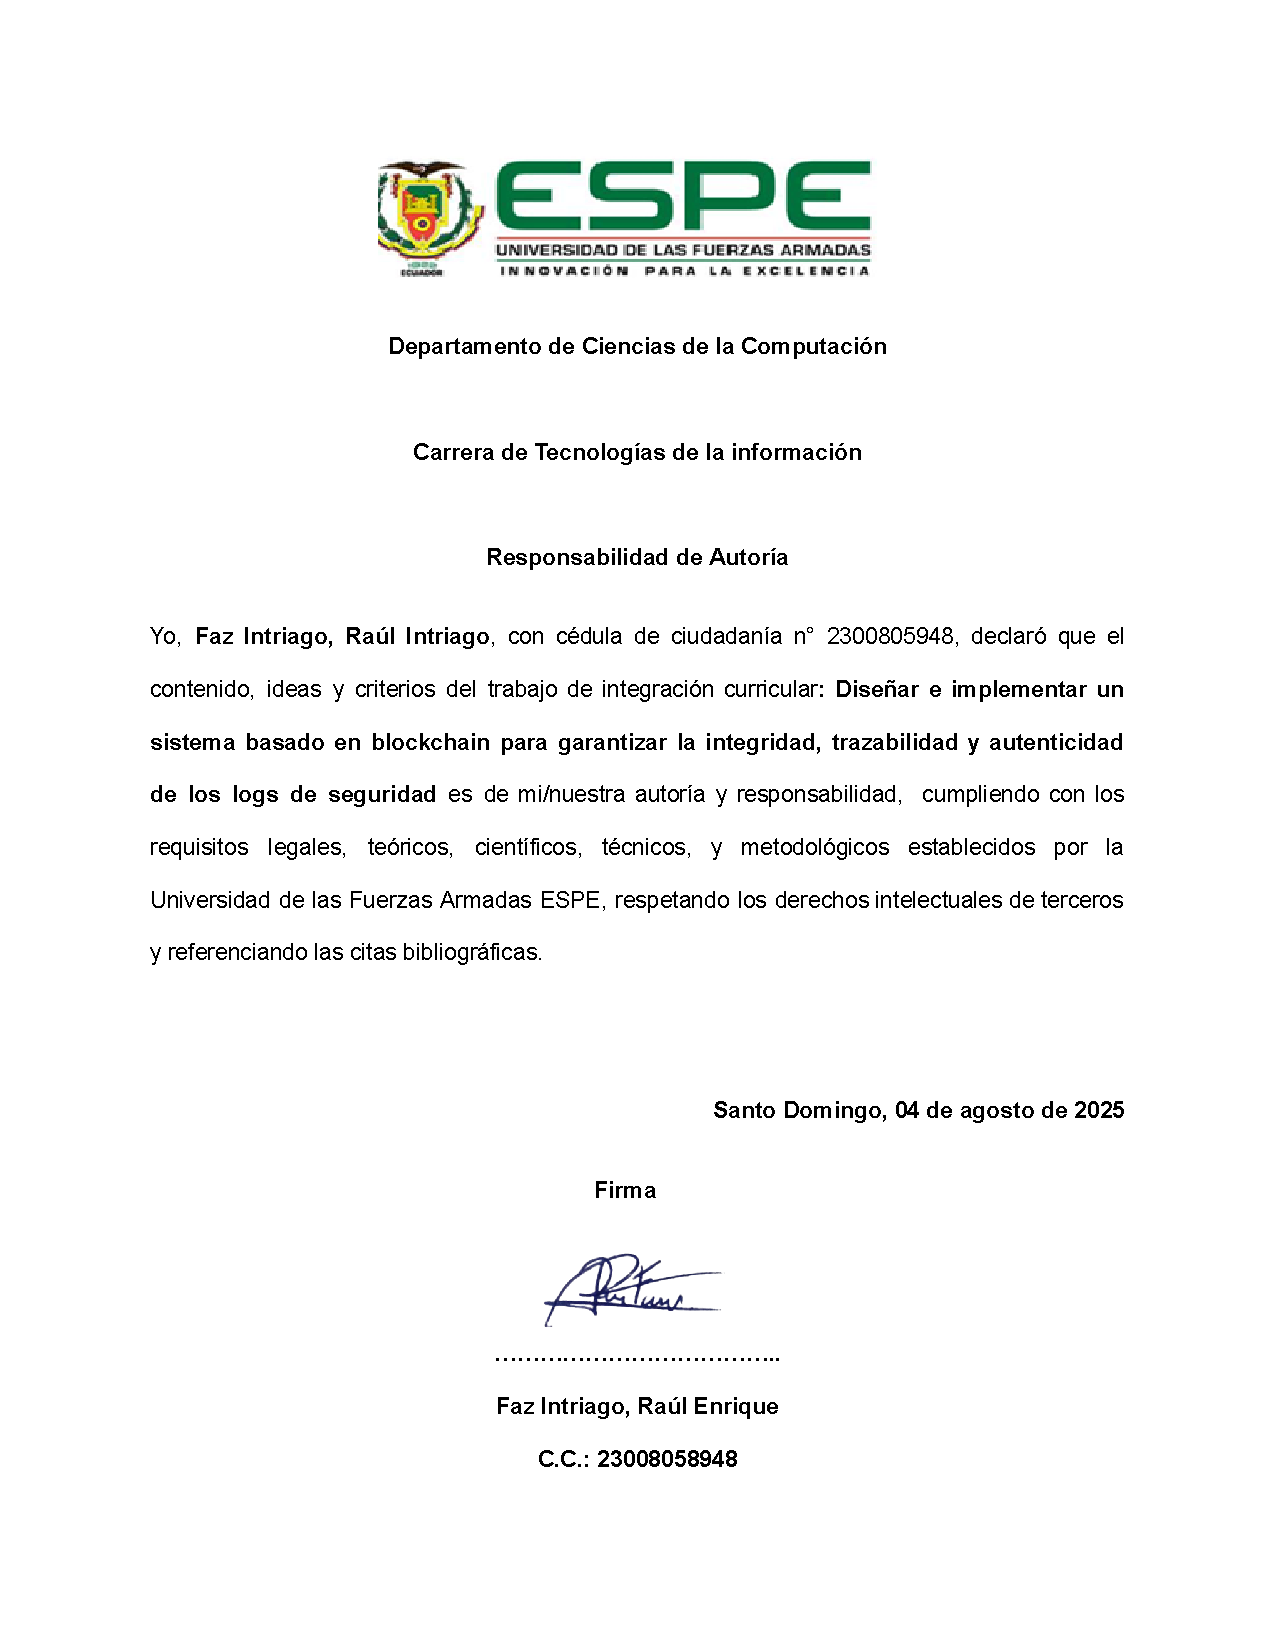
\includepdf[pages=1,fitpaper=true,pagecommand={\thispagestyle{empty}}]{figuras/RF_ResponsabilidadAutoria.pdf}
\newpage

% Autorización de publicación firmada por el tesista
%\phantomsection
%\addcontentsline{toc}{section}{Autorización de Publicación}
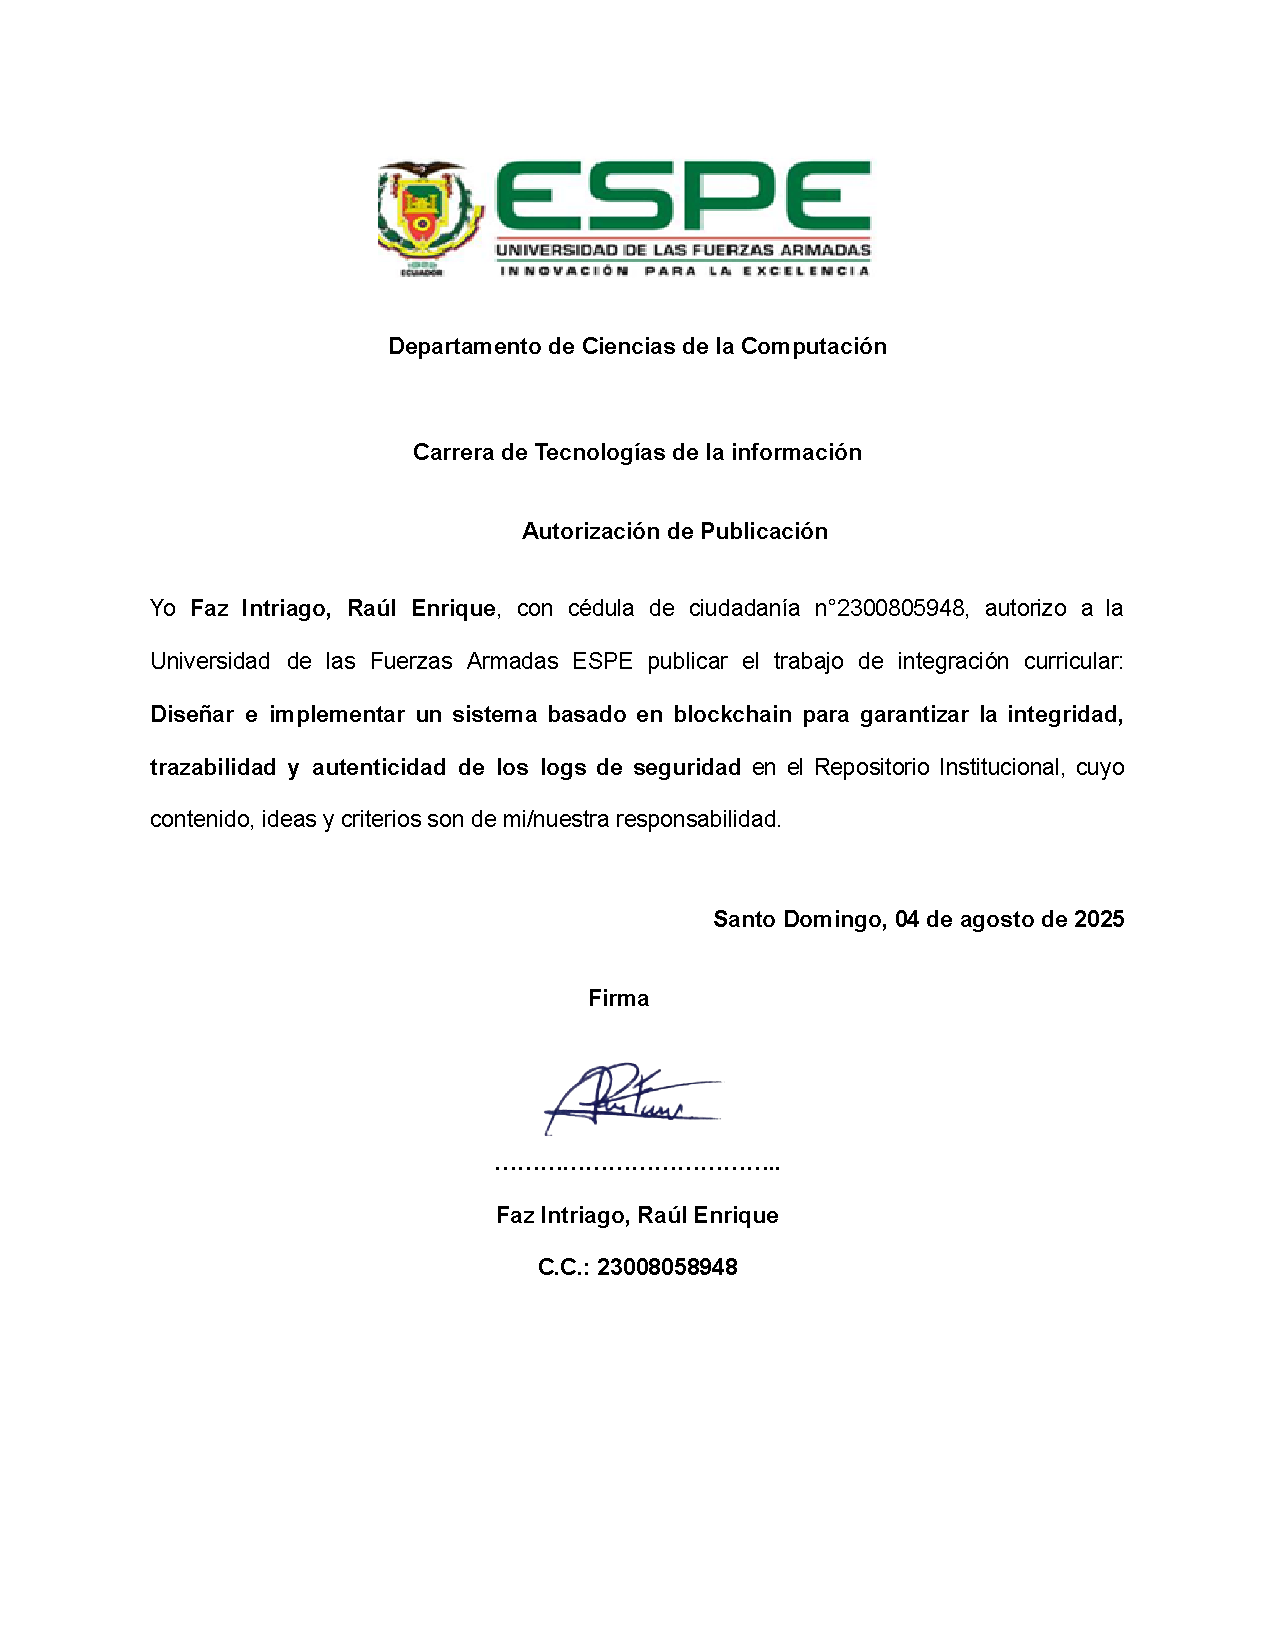
\includepdf[pages=1,fitpaper=true,pagecommand={\thispagestyle{empty}}]{figuras/RF_AutorizacionPublicacion.pdf}
\newpage

\pagenumbering{roman}
\setcounter{page}{1}
% Dedicatoria 
\phantomsection
\addcontentsline{toc}{section}{Dedicatoria}
\renewcommand{\thesection}{\Roman{section}}
\section*{\normalsize \centering{Dedicatoria}}
A lo largo de este camino académico, he tenido el privilegio de compartir experiencias, desafíos y aprendizajes con personas extraordinarias que han marcado de manera significativa mi desarrollo, tanto profesional como personal.

Quiero expresar mi más sincero agradecimiento a mis compañeros de carrera: Josue B., Josué E., Brandon, Laylin, Jair, Lesly, Mónica, Mayerly, Christian, Andrick, Luis, Jhanira, Melany, Steeven R. y Steven V.  Gracias por su compañerismo, por las incontables horas compartidas entre clases, proyectos y desvelos, y por su apoyo constante y sus palabras de aliento. Cada uno de ustedes ha aportado algo único a este proceso, y me siento verdaderamente agradecido de haber recorrido este trayecto en su compañía.

Este logro no habría tenido el mismo valor sin su presencia. Confío en que nuestras trayectorias profesionales se volverán a cruzar y que el lazo que nos une permanecerá firme, más allá de las aulas y del paso del tiempo.

% In Memoriam en la misma página (sin \newpage)
\vspace{1.5cm}  % Menos espacio entre secciones

\begin{center}
{\normalsize \textbf{IN MEMORIAM}}
\end{center}

\begin{flushright}
\begin{minipage}{0.6\textwidth}
\textit{En memoria de mi amado padre, Luis Faz, quien con su ejemplo me enseñó que la vida no siempre es fácil, pero que siempre vale la pena seguir adelante. Su fortaleza ante las adversidades, su esfuerzo constante y su forma de enfrentar la vida me marcaron profundamente y hoy son parte de lo que soy. Aunque ya no esté físicamente conmigo, su recuerdo vive en cada paso que doy y su legado me inspira a nunca rendirme. Donde quiera que estés, papá, gracias por enseñarme a luchar con dignidad y por ser mi inspiración eterna.}
\end{minipage}
\end{flushright}
\vspace{1cm}
\begin{flushright}
Faz Intriago, Raúl Enrique
\end{flushright}

\newpage

% Agradecimientos 
\phantomsection
\addcontentsline{toc}{section}{Agradecimiento}
\section*{\normalsize \centering{Agradecimiento}}
%\begin{center}
%{\large AGRADECIMIENTO}
%\end{center}
Deseo comenzar expresando mi más sincero agradecimiento a mi tutor de tesis, el Ing. Alberto Daniel Núñez Agurto, PhD., por su acompañamiento constante y por compartir generosamente su vasto conocimiento a lo largo de este proceso académico.

Extiendo también mi agradecimiento a los docentes de mi carrera, quienes me brindaron las herramientas, el conocimiento y la orientación necesarios para desarrollar esta investigación con solidez y compromiso.

A mi madre, Cecilia Intriago, le agradezco profundamente por su apoyo incondicional y por ser mi principal fuente de fortaleza durante cada etapa de este camino.

A mi hermana, Andrea Faz, gracias por estar presente en cada momento, por motivarme con tu ejemplo y por ser una inspiración constante para seguir adelante.



\begin{flushright}
Faz Intriago, Raúl Enrique
\end{flushright}



\newpage

\pagestyle{empty}
% Índices
% Contenido
\renewcommand\contentsname{\normalsize ÍNDICE}
\tableofcontents
\setcounter{tocdepth}{2}
\newpage

% Tablas
\renewcommand{\listtablename}{\normalsize ÍNDICE DE TABLAS}
\listoftables
\newpage

% Figuras
\renewcommand{\listfigurename}{\normalsize ÍNDICE DE FIGURAS}
\listoffigures
\newpage

\pagestyle{fancy}
% Resumen de la tesis en español
\pagenumbering{arabic}
\setcounter{page}{1}
\phantomsection
\addcontentsline{toc}{section}{Resumen}
\addcontentsline{toc}{section}{Palabras clave}
\section*{Resumen}
%\section*{RESUMEN}

\noindent
La gestión y auditoría de logs de seguridad constituye un desafío crítico en ciberseguridad moderna, especialmente en organizaciones que manejan información sensible y requieren cumplimiento normativo estricto, donde los sistemas tradicionales presentan vulnerabilidades fundamentales en términos de integridad, inmutabilidad y trazabilidad que limitan significativamente la capacidad para detectar, investigar y responder eficazmente ante incidentes de seguridad. Esta investigación desarrolla e implementa una solución innovadora basada en tecnología blockchain utilizando Hyperledger Fabric como plataforma permisionada para garantizar la gestión segura, inmutable y verificable de logs de seguridad mediante una arquitectura multi-organización que comprende dos entidades especializadas: LogProvider, responsable de la generación, filtrado y almacenamiento de logs mediante protocolos UDP y rsyslog, y LogAuditor, encargada de la verificación criptográfica y auditoría de registros históricos. El sistema integra certificados digitales X.509, bases de datos CouchDB para persistencia, smart contracts desarrollados en Node.js que definen las reglas de negocio para registrar, consultar y auditar eventos de seguridad, incorporando mecanismos avanzados de autenticación mediante firmas digitales SHA-256, eliminación de duplicados por hash MD5, y metadatos enriquecidos que incluyen marcas de tiempo precisas, identificadores únicos y contexto de seguridad. La implementación exitosa demuestra la viabilidad técnica de la solución propuesta, confirmando que la tecnología blockchain permisionada puede garantizar la inmutabilidad y autenticidad de logs de seguridad mediante mecanismos criptográficos robustos, eliminando los puntos únicos de falla presentes en sistemas centralizados tradicionales y proporcionando un entorno distribuido resistente a manipulaciones maliciosas y alteraciones no autorizadas. La solución desarrollada presenta características de escalabilidad horizontal, interoperabilidad con infraestructuras existentes, y adaptabilidad a diversos entornos organizacionales, contribuyendo al campo de la ciberseguridad mediante un framework práctico y replicable que establece un nuevo paradigma para la gestión confiable de logs de seguridad en entornos empresariales críticos
\vspace{10pt}
\noindent\textbf{\emph{Palabras clave:}} {Blockchain, Hyperledger Fabric, Logs de Seguridad, Auditoría, Inmutabilidad, Ciberseguridad, Smart Contracts, Trazabilidad.}
\newpage

% Resumen de la tesis en inglés
\phantomsection
\addcontentsline{toc}{section}{Abstract}
\addcontentsline{toc}{section}{Keywords}
\section*{Abstract}
%\section*{ABSTRACT}

\noindent
Security log management and auditing constitutes a critical challenge in modern cybersecurity, especially in organizations handling sensitive information requiring strict regulatory compliance, where traditional systems present fundamental vulnerabilities in terms of integrity, immutability, and traceability that significantly limit the capability to detect, investigate, and effectively respond to security incidents. This research develops and implements an innovative solution based on blockchain technology using Hyperledger Fabric as a permissioned platform to guarantee secure, immutable, and verifiable security log management through a multi-organization architecture comprising two specialized entities: LogProvider, responsible for generation, filtering, and storage of logs via UDP protocols and rsyslog, and LogAuditor, in charge of cryptographic verification and auditing of historical records. The system integrates X.509 digital certificates, CouchDB databases for persistence, smart contracts developed in Node.js that define business rules for recording, querying, and auditing security events, incorporating advanced authentication mechanisms through SHA-256 digital signatures, MD5 hash-based duplicate elimination, and enriched metadata including precise timestamps, unique identifiers, and security context. The successful implementation demonstrates the technical viability of the proposed solution, confirming that permissioned blockchain technology can guarantee immutability and authenticity of security logs through robust cryptographic mechanisms, eliminating single points of failure present in traditional centralized systems and providing a distributed environment resistant to malicious manipulations and unauthorized alterations. The developed solution presents horizontal scalability characteristics, interoperability with existing infrastructures, and adaptability to diverse organizational environments, contributing to the cybersecurity field through a practical and replicable framework that establishes a new paradigm for reliable security log management in critical enterprise environments.

\vspace{10pt}
\phantomsection
\noindent\textbf{\emph{Keywords:}} {Blockchain, Hyperledger Fabric, Security Logs, Auditing, Immutability, Cybersecurity, Smart Contracts, Traceability.}
\newpage

% Capitulos
\section{Introducción y estado del arte}

\subsection{Introducción}
En la era digital actual, los sistemas de información se enfrentan a una constante amenaza a su integridad y seguridad, lo que hace imperiosa la implementación de mecanismos para la recolección, almacenamiento y verificación de eventos críticos. Los logs de seguridad juegan un papel importante, pero su gestión tradicional presenta desventajas, como la manipulación, falsificación y pérdida de registros, sobre todo si se almacenan en servidores centralizados ~\cite{birk2011forensics}.

Para responder a estos retos, la tecnología blockchain surge como una nueva alternativa para permitir una infraestructura funcional y descentralizada, una estructura que es transparente y resistente a la manipulación. La blockchain, que apareció inicialmente como la tecnología que dio lugar a Bitcoin ~\cite{nakamoto2008bitcoin}, ha evolucionado para abarcar áreas como la ciberseguridad, gracias a propiedades como la inmutabilidad, la distribución de confianza y la trazabilidad, respaldadas por funciones criptográficas como los hashes y estructuras de datos como los Merkle Trees~\cite{crosby2016blockchain,stallings2017crypto}.

La incorporación de blockchain para gestionar logs de seguridad hace que no sólo aumente la integridad de los datos que se almacenan en ellos, sino que permite la posibilidad de auditar fácilmente los eventos que se registran lo que permite su verificación criptográfica sin necesidad de terceros. Además, el uso de algoritmos de consenso y mecanismos de validación distribuidos permite asegurar que los registros ya no pueden ser alterados una vez se encuentran en la cadena ~\cite{zheng2017overview}.

Durante la evolución de la blockchain, se han ido produciendo distintas arquitecturas (públicas, privadas y de consorcio por citar sólo unas cuantas) que se adaptan a las particularidades de cada entorno y a los objetivos de entornos empresariales o institucionales ~\cite{christidis2016blockchains}. En este sentido, diseñar un sistema que combine los principios de la blockchain a las necesidades concretas de logs de seguridad es una buena oportunidad de mejorar grandemente la seguridad de nuestros procesos, así como la transparencia y la confianza en procesos de vigilancia y auditoría digital.

El trabajo que se presenta tiene como objetivo el diseño y la implementación de un sistema de logs de seguridad basado en blockchain que garantice la integridad, la trazabilidad y la autenticidad de los logs de seguridad, siempre con un enfoque que permita la evaluación en términos de aplicabilidad. Esta tesis pretende colaborar al fortalecimiento de los mecanismos de defensa de infraestructuras críticas, incorporando los avances tecnológicos en la cuestión de los logs distribuidos.



\subsection{Estado del arte}
Es crucial confirmar la necesidad de revisión, según el requisito básico es la identificación de la problemática del proyecto. Por medio de este proceso se recogen las investigaciones existentes y, con este fin , se pone énfasis en aspectos importantes para el diseño e implementación de un sistema que garantice la integridad, trazabilidad y autenticidad de los logs de seguridad utilizando tecnología blockchain.

%%%%%%%%%%%%%%%%%%%%%%%%%%%%%%%%%%%%%%%%%%%%
Los criterios de inclusión empleados para identificar estudios relacionados con la presente investigación son:
\begin{itemize}
    \item Trabajos relacionados con el uso de blockchain en el ámbito de la seguridad informática.
    \item Investigaciones que aborden la gestión, integridad o trazabilidad de logs de seguridad.
    \item Artículos que incluyan el uso de smart contracts o chaincode en su propuesta.
    \item Publicaciones de los últimos 6 años (2019–2025).
    \item Artículos disponibles en inglés.
\end{itemize}

Por otro lado, los criterios de exclusión establecidos son:
\begin{itemize}
    \item Investigaciones que no incluyan componentes relacionados con blockchain o seguridad de logs.
    \item Trabajos que no presenten una metodología clara.
    \item Artículos no disponibles en texto completo.
\end{itemize}

Para la búsqueda de toda la información relacionada con esta investigación, se revisaron documentos, artículos científicos y conferencias indexadas en bases de datos académicas como IEEE Xplore. La cadena de búsqueda empleada fue la siguiente:

(security OR “information security” OR cybersecurity) AND (blockchain OR block-chain OR “distributed ledger technology”) AND (logs OR logfile OR “security events”) AND (integrity OR traceability OR authenticity OR immutability) AND (“smart contracts” OR chaincode)

Al aplicar esta cadena de búsqueda en IEEE Xplore, se obtuvieron 14 resultados. De estos, se seleccionaron los artículos que cumplían con los criterios de inclusión y aportaban valor a la presente investigación, los cuales fueron 5 serán analizados a continuación.

\subsubsection{Elaboración del estado del arte}

\textbf{EP1.}  El artículo científico elaborado por~\cite{8804170}  titulado \textbf{“Smart Contract-Based Product Traceability System in the Supply Chain Scenario”}, presenta una solución innovadora que utiliza blockchain y smart contracts para asegurar la integridad, trazabilidad y autenticidad de los registros en una cadena de suministro.

Este esquema de trabajo se hace funcionar implementando un procedimiento para ir registrando, de forma irreversible, el conjunto de cada evento y movimiento de un producto en un libro mayor distribuido. De este modo, las auditorías son completamente transparentes, la veracidad de la información no queda en entredicho.
Los acuerdos inteligentes hacen los pasos por sí mismo y adeguran que las transacciones sean seguras, mientras que un aparato de identificación hace más fuerte la protección del sistema.

También, todos los datos de los hechos del sistema están en la red cadena, lo que los salvaguarda de cambios y cuida su forma correcta. Esto deja hacer revisiones seguras desde cualquier máquina que pueda entrar a internet, al mismo tiempo que da un control claro de cada uno de los movimientos hechos.

El grado de viabilidad de la propuesta quedó demostrado al aplicar el sistema de forma práctica con frameworks como Truffle, explicitando cómo implantarlo en redes locales. Ello pone de manifiesto el potencial que puede acoger la metodología de blockchain para operar con registros críticos en forma de datos, sirviendo de base para la elaboración de sistemas de confianza capaces de funcionar en distintas modalidades, muy en especial en la operación con logs de seguridad. 


%%%%%%%%%%%%%%%%%%%%%%%%%%%%%%%%%%%%%%%%%%%%%%%
\textbf{EP2.}  El artículo científico elaborado por~\cite{sheng2023blockchain}  titulado \textbf{“Blockchain-Based Traceability for Teak Identity: A Transformational Approach”}, nos presenta una solución fascinante: usar la blockchain de Ethereum para asegurar la trazabilidad de la teca a lo largo de toda su cadena de suministro.

En este estudio, los autores crearon e implementaron smart contracts en Solidity que son capaces de almacenar, de forma inmutable, todos los metadatos relacionados con el origen y el movimiento de la madera. ¿El resultado? La integridad y autenticidad de la información quedan totalmente garantizadas.

Este método no solamente da vista en vivo y revisión rápida de información, pero también quita la necesidad de usar papeles. Esto, claro, baja muy fuerte el peligro de cambios o engaños en los registros. Ademñas, al probar la solución en redes de prueba como Rinkeby y Ropsten, los autores confirmaron que esta tecnología es viable ttno técnica como económicamente.


%%%%%%%%%%%%%%%%%%%%%%%%%%%%%%%%%%%%%%%%%%%%%%%%%
\textbf{EP3.}  El artículo científico elaborado por~\cite{Patel2024FuzzyEnhanced}  titulado \textbf{“Fuzzy-Enhanced Secure Messaging Framework for Smart Healthcare System”}.  El presente artículo nos revela una propuesta realmente innovadora: un sistema destinado a facilitar la compartición segura de datos en un entorno de salud inteligente con datos provenientes de la inteligencia artificial (IA), la lógica difusa y la tecnología blockchain. Pese a que se trata de datos médicos, la metodología es muy versátil y puede ser aplicada en cualquier ámbito donde la integridad y autenticidad de los datos  como por ejemplo, en los registros de seguridad importantes. 

¿Cómo hace eso? La IA clasifica los datos para determinar si estos son maliciosos. Solo aquellos datos que no representan una amenaza son los que se guardan en la blockchain. Este filtrado previo es clave porque asegura que solo la información válida y confiable se registre de forma inmutable. La blockchain, por su parte, garantiza la integridad y la resistencia a cualquier manipulación gracias a herramientas como los Merkle Trees y las firmas digitales únicas.

Para controlar quién puede ver qué, se usan smart contracts. Son como vigilantes digitales que chequean quien tiene permiso para mirar los datos, permitiendo solo a usuarios autorizados ver la información guardada. Este sistema de identificación y aprobación es muy útil en los logs de seguridad, donde cuidar el acceso a estos registros es tan clave como asegurar que su info no sea cambiada. 

A pesar de que la investigación que aquí se presenta no toma los logs de red o de sistema como objeto de estudio, sí que deja una carga de ideas muy potentes con respecto a la importancia de preproceso de la información antes del registro y la propia idea de cómo los smart contracts pueden ser  una potente herramienta para una buena gestión del acceso a datos sensibles de forma verificada y segura.

%%%%%%%%%%%%%%%%%%%%%%%%%%%%%%%%%%%%%%%%%%%%%%%%%%
\textbf{EP4.}  El artículo científico elaborado por~\cite{MorilloReina2025Decentralized}  titulado \textbf{“Decentralized and Secure Blockchain Solution for Tamper-Proof Logging Events”}. Este trabajo está alineado con nuestra línea de investigación ya que propone una solución sobre blockchain para lograr la integridad, la inmutabilidad y el no repudio de los sucesos de log. También indican la importancia de los logs en la seguridad de la información, como método de detección de incidentes, auditoría, análisis forense y en cumplimiento de normas; aunque igualmente reconocen cuán complicado es poder garantizar su integridad ante manipulaciones, sean internas o externas.

La brillante propuesta de la investigación en cuestión consiste en llevar a cabo el registro en una blockchain de la forma de resguardo de los hashes de los eventos de log. Esto es, porque a la hora de implementar la blockchain, se está utilizando dicha propiedad como una manera más de asegurar el evento en un registro inmutable. Según el mecanismo de la red de blockchain que se esté utilizando, el evento puede guardarse directamente como metadato (aunque dependerá de la plataforma para que esto sea posible) o bien puede generarse el HMAC con el ID de la transacción y luego enlazarlo al evento accediendo al registro de un servidor de gestión de logs.

Un evento log almacenado en la blockchain es incambiable e irrefutable, garantizando su propia inmutabilidad, ya que la blockchain incorpora la información de un modo escalonado y cronológico mejorando mucho la trazabilidad de los logs. Esta verificación se vuelve pública y transparente, lo que facilita las auditorías y evita que se niegue la existencia o el contenido de un log (el famoso no repudio), ya que su huella digital queda certificada con una marca de tiempo inalterable.

%%%%%%%%%%%%%%%%%%%%%%%%%%%%%%%%%%%%%%%%%%%%%%%%%%
\textbf{EP5.}  El artículo científico elaborado por~\cite{Pourvahab2019Efficient}  titulado \textbf{“An Efficient Forensics Architecture in Software-Defined Networking-IoT Using Blockchain Technology”}. Este artículo nos presenta una arquitectura forense que, según su autor, resulta muy atractiva. Está articulada alrededor de entornos de redes definidas por software (SDN) y de dispositivos IoT, utilizando para ello la tecnología blockchain para proteger y asegurar la evidencia digital, como los logs de eventos y otros datos.

Pese a que el objetivo principal de esta propuesta tiene su base en la informática forense, la idea que presenta es super útil para la gestión segura de logs en cualquier ámbito. Para proteger la integridad de los datos que son objeto de la explotación de los logs, los controladores SDN computan un hash de cada log y lo almacenan en la blockchain. Esto es clave ya que, una vez incorporados, el log no puede ser manipulado ni eliminado, es decir, han sido censados, ¡Y eso es como derecho! Podríamos decir que se les ha incorporado un candado digital que permite reforzar la Cadena de Custodia (CoC), al permitir preservarlos desde el momento que han sido recolectados hasta el que han sido analizados.

En lo que se refiere a su autenticidad para garantizarlo el sistema hace uso de firmas homomórficas y claves únicas basadas, en las llamadas, curvas elípticas, algo que permite comprobar que los logs provienen de dispositivos y usuarios legítimos. Además, para acceder a estos logs hay que autenticarse lo que garantiza que solo las personas autorizadas pueden revisarlos. 

La trazabilidad de los logs está garantizada gracias a la inmutabilidad propia de la tecnología blockchain. Esto permite almacenar registros de cualquier procedencia, incluyendo información como la hora, la dirección y la localización. Todo con la posibilidad de poder rastrear la proveniencia sin que el riesgo de la manipulación de los logs se interponga. Resumiendo, la propuesta aporta con su criterio la manera como la blockchain puede convertirse en un instrumento muy potente para garantizar la integridad, la autenticidad y la trazabilidad de los logs específicamente cuando son considerados como una evidencia forense.

%%%%%%%%%%%%%%%%%%%%%%%%%%%%%%%%%%%%%%%%%%%
\subsection{Objetivos}
\subsubsection{Objetivo General}
Diseñar e implementar un sistema basado en blockchain para garantizar la integridad, trazabilidad y autenticidad de los logs de seguridad


\subsubsection{Objetivos Específicos}
\begin{itemize}
    \item Analizar los métodos tradicionales de almacenamiento y gestión de logs de seguridad, identificando sus limitaciones en términos de integridad, trazabilidad y autenticidad.
    \item Seleccionar y configurar una plataforma blockchain adecuada, para el almacenamiento inmutable de logs de seguridad.
    \item Diseñar e implementar un mecanismo de recolección y envío de logs a la red blockchain.
    \item  Desarrollar una interfaz que permita la consulta, validación y visualización de los logs almacenados en la blockchain.


 
\end{itemize}
%\begin{itemize}

 
%\end{itemize}


\subsection{Alcance}
El presente trabajo aborda el diseño e implementación de un sistema basado en blockchain para la gestión segura de logs de seguridad, utilizando el framework Hyperledger Fabric. La propuesta incluye un análisis comparativo entre los métodos tradicionales de almacenamiento de logs y el uso de tecnología blockchain, así como la construcción de una red multicapa conformada por dos organizaciones: LogProvider y LogAuditor.

Se desarrollan smart contracts para garantizar el registro inmutable de los logs y se integran mecanismos automáticos para la recolección y transferencia de datos desde los sistemas fuente. Además, se implementa una interfaz web que permite consultar, validar y visualizar los registros almacenados, asegurando la trazabilidad mediante funciones de auditoría.

El sistema desarrollado demuestra la viabilidad técnica de blockchain para preservar la integridad, autenticidad y no repudio de los logs, ofreciendo una solución escalable y confiable para la gestión de evidencia digital en entornos empresariales.

\newpage

\section{Marco teórico}
Este capítulo estudia las bases que justifican el diseño de un sistema que utiliza tecnología blockchain para garantizar la integridad, la trazabilidad y la autenticidad de los logs de seguridad. Se analiza la importancia de los logs en los sistemas informáticos y la casuística de aquellos riesgos a los que pueden estar expuestos, en especial, la modificación y/o eliminación de los logs. También se introducen los conceptos más relevantes de la tecnología blockchain y su aplicación en aquellos entornos donde la protección y verificación de los datos es un elemento fundamental.
%%%%%%%%%%%%%%%%%%%%%%%%%%%%%%%%%%%%%%%%%%%%%%%%%%%%%%%%%%%%%%%%%%%%%%%
\subsection{Seguridad Informática}
\subsubsection{Concepto y principios fundamentales}
La seguridad informática se refiere a la protección de los sistemas de información y de sus componentes hardware, software, redes y datos frente a accesos no autorizados, alteraciones, destrucción o divulgación indebida. Esta disciplina ha cobrado relevancia como respuesta al creciente nivel de dependencia de los sistemas digitales y al aumento sostenido de las amenazas cibernéticas. Su objetivo principal es garantizar la confidencialidad, la integridad y la disponibilidad de la información, principios que conforman el modelo conocido como CIA por sus siglas en inglés (Confidentiality, Integrity, Availability)~\cite{Pfleeger2007}.
\begin{itemize}
    \item La confidencialidad significa que la información solo es accesible a aquellos que tienen la autorización correspondiente. Se logra a través de métodos como la criptografía, el control de acceso y la autenticación.
    \item La integridad es la precisión y consistencia de los datos durante el ciclo de vida de la información. Asegúrese a través de la utilización de funciones hash, sumas de comprobación o los logs de auditoría.
    \item La disponibilidad consiste en garantizar que los sistemas informáticos y la información estén accesibles para los usuarios en el momento en que los requieran. Para lograrlo, se implementan mecanismos que permiten mitigar interrupciones en el servicio, como sistemas redundantes, copias de seguridad y planes de recuperación ante desastres~\cite{Stallings2017}.
\end{itemize}
\begin{figure}[H]
    \centering
    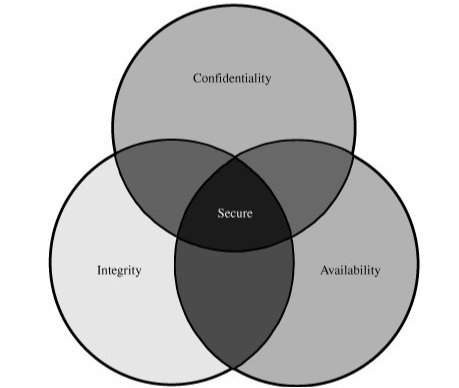
\includegraphics[scale=0.99]{figuras/secure.png}
    \caption{Secure~\cite{Stallings2017}} 
   % \label{fig17}
\end{figure}
A menudo se incorporan otros principios a los tradicionales, como la autenticación, que verifica la identidad de los usuarios; el no repudio, que asegura que una acción o transacción no pueda ser negada por su autor; y la auditoría, que permite rastrear las acciones realizadas dentro del sistema~\cite{Bishop2018}.
Estos principios constituyen la base sobre la cual se diseñan las políticas y mecanismos de seguridad. En el contexto actual, caracterizado por arquitecturas distribuidas, servicios en la nube y tecnologías emergentes como blockchain, la aplicación rigurosa de estos fundamentos resulta esencial para mitigar riesgos y mantener la confianza en los sistemas.

\subsubsection{Amenazas y vulnerabilidades comunes en sistemas de información}
En el ámbito de la seguridad informática, las vulnerabilidades y las amenazas representan los principales riesgos para la integridad, la confidencialidad y la disponibilidad de los sistemas de información. Una amenaza se define como cualquier circunstancia o evento con potencial de causar daño a un sistema o a su información, mientras que una vulnerabilidad corresponde a una debilidad que puede ser explotada por una amenaza para comprometer la seguridad~\cite{Stallings2018}.

Las amenazas se clasifican, en términos generales, en dos categorías: externas e internas. Las amenazas externas provienen de agentes que no forman parte del sistema, como los hackers, el malware, el ransomware, los ataques de denegación de servicio (DDoS) y el phishing. En estos casos, los atacantes suelen aprovechar vulnerabilidades conocidas del software o errores de configuración para infiltrarse en los sistemas~\cite{Pfleeger2007}. Un ejemplo representativo de este tipo de ataques es el ransomware WannaCry, que en 2017 afectó a miles de sistemas a nivel mundial mediante la explotación de una vulnerabilidad en el protocolo SMB de Windows~\cite{Symantec2017}.

Por otro lado, las amenazas internas provienen de usuarios con acceso legítimo a los sistemas, lo que las hace especialmente peligrosas, ya que pueden pasar desapercibidas durante largos periodos. Empleados descontentos, errores humanos o actos negligentes constituyen situaciones comunes asociadas a este tipo de riesgos.

Entre las vulnerabilidades más frecuentes se encuentran las siguientes:
\begin{itemize}
    \item Errores de programación: por ejemplo, desbordamientos de búfer, inyecciones SQL y XSS (cross-site scripting), que permiten ejecutar código malicioso sobre aplicaciones con vulnerabilidades~\cite{OWASP2021}.
    \item Configuraciones incorrectas: servidores mal configurados, puertos abiertos que no deberían estarlo o credenciales por defecto que pueden ser rastreadas y explotadas fácilmente.

    \item Software desactualizado: la falta de actualizaciones y de parches de seguridad incrementan de una forma significativa la posibilidad de explotación de sistemas.

    \item Falta de cifrado de datos: tanto de datos en tránsito como en reposo, la ausencia de cifrado permite hacer volar todo tipo de datos.

    \item Ingeniería social, ataques que manipulan psicológicamente a los usuarios para provocar que faciliten claves o acceso a sistemas.
    
\end{itemize}

La combinación de amenazas y vulnerabilidades dan lugar a los vectores de ataque, es decir, caminos o modos específicos para que un atacante pueda comprometer un sistema. Un ataque típico es enviar un correo de phishing que contiene un enlace a una página falsa (amenaza), aprovechándose de que el usuario no tiene un sistema de verificación multifactor (vulnerabilidad) para robar credenciales de acceso.
En respuesta, las organizaciones deben implantar estrategias proactivas como son auditorías de seguridad, pruebas de penetración, formación continua del personal y políticas estrictas de control de acceso. A partir de este aspecto, es especialmente interesante la utilización de tecnologías emergentes como blockchain para mejorar la trazabilidad y autenticidad de los eventos, lo cual puede suponer una línea de defensa adicional ante modificaciones maliciosas de registros críticos como logs~\cite{Crosby2016}.

\subsubsection{Autenticación, autorización y auditoría}

Los conceptos de autenticación, autorización y auditoría son el fundamento básico para la defensa de los sistemas de información. Con ellos se persigue que los recursos sólo sean utilizados por usuarios válidos y que se pueda registrar las acciones que realiza para su revisión posterior.

La autenticación es la acción a partir de la cual un sistema valida si un usuario o entidad es lo que dice ser. Esto se consigue a través del uso de credenciales clásicas (contraseñas), de tokens, de biometría o de sistemas multifactor, en combinación con al menos dos métodos de verificación~\cite{Stallings2017}.

La autorización, en cambio, se refiere a la posibilidad de poder otorgar permisos a usuarios autenticados y cómo se pueden utilizar los recursos o bien con qué privilegios. Los modelos más utilizados son el control de acceso basado en roles (RBAC) y el control de acceso basado en atributos (ABAC)~\cite{Sandhu1996}.

La auditoría garantiza la obtención, monitorización y análisis de los eventos y actividades del sistema. Su objetivo es detectar comportamientos irregularidad, buscar ataques y permitir la trazabilidad. Un sistema de auditoría óptimo es necesario para el cumplimiento de las normas de seguridad y para la reconstrucción de los incidentes tras una brecha~\cite{Bishop2018}.

Cuando se aplican adecuadamente estos tres mecanismos suponen una importante capa defensiva de cualquier infraestructura tecnológica contemporánea.


%%%%%%%%%%%%%%%%%%%%%%%%%%%%%%%%%%%%%%%%%%%%%%%%%%%%%%%%%%%%%%%%%
\subsection{Blockchain}
\subsubsection{ Origen y evolución del blockchain}
La idea de blockchain aparece como una forma de poder registrar las transacciones de forma segura, descentralizada y resistente a la manipulación. Esta idea toma su origen en el artículo que publicó el conocido pseudónimo de Satoshi Nakamoto en 2008 con el que se propuso una moneda digital, el Bitcoin, que estaba estructurada sobre una forma de datos encadenados cronológicamente de la que se hablaba como de cadena de bloques~\cite{nakamoto2008bitcoin}, lo cual servía para poder registrar transacciones entre pares sin la necesidad de tener un ente central que se hiciera cargo de ello y permitía así resolver el problema de los dobles gastos en entornos digitales.
A pesar de que el término “blockchain” suena en relación a Bitcoin, su antecedente teórico se remonta a décadas pasadas, en 1991 Stuart Haber y W. Scott Stornetta proponían un método mediante el cual se pudiera certificar la inmutabilidad de los documentos digitales recurriendo a un sistema de sellado de tiempo que fuera criptográfico~\cite{Haber1991}. Posteriormente, en el año 1997, las partes interesadas introdujeron el concepto de árboles de Merkle, que permiten verificar conjuntos de datos muy grandes con una mayor eficiencia.
La historia del blockchain ha acometido distintas etapas relevantes. En primer lugar, la primera generación de blockchain, representada por Bitcoin, introdujo transacciones financieras completamente descentralizadas. Esta implementación demostró la capacidad de mantener registros inmutables sin depender de un intermediario de confianza; no obstante, su funcionalidad se limitaba a operaciones predefinidas.~\cite{nakamoto2008bitcoin}.

\begin{figure}[h!]
\centering
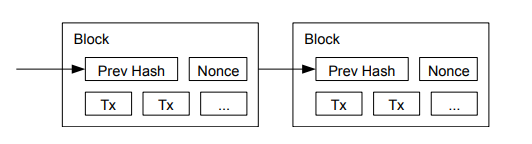
\includegraphics[width=0.7\textwidth]{figuras/blockchain.png} 
\caption{Estructura básica de una blockchain \cite{nakamoto2008bitcoin}}
\label{fig:blockchain_estructura}
\end{figure}
La Figura~\ref{fig:blockchain_estructura} ilustra la estructura fundamental de una blockchain, tal como fue concebida originalmente~\cite{nakamoto2008bitcoin}. Cada bloque contiene un puntero al hash del bloque anterior denominado \textit{“Prev Hash”} lo que garantiza la continuidad y el orden dentro de la cadena. Además, incorpora un conjunto de transacciones (Tx) que han sido validadas y añadidas al registro. El campo “Nonce” es un número aleatorio que los mineros modifican durante el proceso de Proof of Work hasta encontrar un hash que cumpla con los criterios establecidos por la red. Una vez se encuentra un hash válido, este se incluye en el bloque y, posteriormente, se incorpora como referencia en el siguiente bloque, conformando así una cadena inalterable y resistente a manipulaciones.

Tras ello, en 2015, con la llegada de Ethereum comenzó la segunda generación de blockchain, que permitió la creación de los smart contracts, programas que se ejecutan automáticamente, se almacenan en la cadena de bloques y se activan siempre que se cumplan ciertas condiciones~\cite{Buterin2014}. Esta innovación amplió enormemente las aplicaciones de la blockchain, incluyendo la automatización de procesos jurídicos, financieros o logísticos, entre otros.

Actualmente, se habla de una tercera generación de blockchain, representada por plataformas como Cardano, Polkadot o Algorand, que intentan solucionar los problemas de escalabilidad, interoperabilidad y eficiencia energética a medida que buscan no sacrificar la descentralización ni la seguridad~\cite{Swan2015}. Estas plataformas emplean algoritmos de consenso más sofisticados, como Proof of Stake (PoS) o Byzantine Fault Tolerance (BFT), en contraposición al intensivo mecanismo Proof of Work (PoW) de Bitcoin.

Además, han surgido distintos tipos de blockchain según su nivel de acceso y gobernanza: públicas (abiertas y descentralizadas), privadas (exclusivas para ciertos entes) y consorciadas (autogestionadas por un grupo de organizaciones)~\cite{Xu2017}. La diversidad de estas plataformas ha facilitado su adopción en ámbitos como la salud, la educación, la logística y, de forma destacada, la ciberseguridad, donde se utilizan para mejorar la trazabilidad e integridad de la información, por ejemplo en los logs de seguridad.

La blockchain ha evolucionado de ser una solución financiera descentralizada a convertirse en un marco versátil con aplicaciones transversales en múltiples sectores. Su crecimiento ha acompañado tanto el avance tecnológico como la demanda de sistemas confiables, transparentes e inmutables en entornos donde la integridad de los datos resulta crítica.

\subsubsection{ Arquitectura de blockchain (bloques, cadena, nodos)}
La arquitectura de una blockchain se basa en una estructura de datos distribuida especialmente diseñada para el registro inmutable de transacciones. Esta arquitectura está compuesta fundamentalmente por bloques, que se enlazan de forma secuencial formando una cadena, y por una red de nodos que participan en el mantenimiento y la validación de dicha cadena.

Cada bloque contiene un conjunto de transacciones agrupadas junto con información adicional, generalmente denominada metadatos. Entre estos metadatos se incluyen el hash del bloque anterior, la marca de tiempo (fecha y hora), y en blockchains basadas en el mecanismo de Proof of Work, un valor denominado nonce (un número aleatorio que los mineros modifican para encontrar un hash válido). Estos elementos permiten garantizar la integridad y seguridad de la cadena. 

El encabezado de un bloque no solo incluye el hash del bloque anterior, la marca de tiempo y el nonce, sino también un resumen hash de todas las transacciones, generalmente mediante un árbol de Merkle. Esto permite verificar de forma eficiente la integridad individual de las transacciones, sin necesidad de revisar todo el contenido del bloque~\cite{Stallings2017}. Esta organización se encarga de garantizar que cualquier alteración a los datos de un bloque altere su respectivo hash, quebrando la conexión con el siguiente bloque y, como consecuencia, el hecho de que los datos han sido alterados.

La cadena de bloques es el resultado del enlazado criptográfico y en orden temporal de los bloques. Esta función de encadenar los bloques mediante hashes permite asegurar la inmutabilidad del historial de transacciones, ya que se requiere rehacer todos los hashes de los bloques posteriores al que haya sido alterado y, además, obtener el consenso de la red, lo cual resulta computacionalmente inviable en blockchains públicas con mecanismos como Proof of Work o Proof of Stake~\cite{nakamoto2008bitcoin}.

Los nodos son las entidades que actúan dentro de la red blockchain. El tipo de nodo y el tipo de blockchain determinan las funciones que puede desempeñar. Así, existen nodos que solo almacenan copias del libro mayor (nodos ligeros) y otros que participan activamente en el consenso, validando transacciones y agregando bloques al libro mayor (nodos validadores o mineros)\cite{Swan2015}. Del mismo modo, en redes como Hyperledger Fabric, los nodos tienen roles específicos: peers, que almacenan los libros mayores y ejecutan smart contracts; orderers, que garantizan el orden de las transacciones; o clients, que inician las solicitudes\cite{HyperledgerFabric2.5KeyConcepts}.

En el caso de blockchains permisadas como Hyperledger Fabric, la arquitectura de red permite una mayor modularidad y control sobre quién puede actuar como nodo y qué operaciones puede realizar. A diferencia de las cadenas públicas, donde cualquier usuario puede convertirse en nodo, en las blockchains empresariales se aplican políticas de acceso basadas en identidades verificadas y certificados digitales~\cite{HyperledgerFabric2.5KeyConcepts}. Por lo tanto, toda interacción entre bloques, la cadena criptográfica y los nodos participantes se realiza en un entorno de confianza sin intermediarios. Este tipo de arquitectura es ideal para casos en los que se requiere garantizar integridad y trazabilidad, como en la gestión de logs de seguridad.



\subsubsection{Propiedades principales: inmutabilidad, descentralización, transparencia}

Las características más importantes que permiten la diferenciación de blockchain son la inmutabilidad, la descentralización y la transparencia, presentando las bases garantizadoras de su fiabilidad y de la posibilidad de aplicarse en entornos donde la seguridad y la trazabilidad son las premisas a cumplir.

La inmutabilidad hace referencia a que, cuando los datos están ya registrados en la cadena de blocks, parezca prácticamente imposible su modificación. Tal característica se garantiza por medios de técnicas criptográficas como son las funciones hash y la estructura de encadenado de los blocks. Esto permite que cualquier tentativa de modificación sea identificada fácilmente~\cite{Stallings2017}.

La descentralización, por el contrario, no requiere de una entidad central a la que se le pueda dar confianza. Más bien, una vez más, la validación y almacenamiento de la información se distribuyen y llevan a cabo por muchos nodos que forman parte de la red. Como resultado, el aumento en la tolerancia a errores se verá ocultado de igual manera por la disminución de posibilidades de censura o manipulación de la información~\cite{nakamoto2008bitcoin}.

La transparencia lleva a los participantes afines a poder comprobar el estado y la historia de las transacciones, incrementando la posibilidad de confianza en un sistema colaborativo. La visibilidad será variable según sea el tipo de blockchain que incluyamos (público o privado), pero la certeza de la trazabilidad de los hechos sometidos a verificación será constante~\cite{Crosby2016}.
Estas características hacen que blockchain pueda considerarse como un elemento adecuado para poder asegurar la integridad y autenticidad de la información sensible como podrían ser el caso de los logs de seguridad.

\subsubsection{Funciones hash y su importancia en blockchain}
Las funciones hash criptográficas constituyen uno de los pilares fundamentales de la tecnología blockchain, ya que permiten transformar una entrada de datos de cualquier longitud en una salida de longitud fija, denominada hash o digest. Esta salida es única para cada entrada diferente, de modo que incluso una mínima alteración en los datos originales genera un hash completamente distinto~\cite{bishop2003computer}.

En el contexto de blockchain, las funciones hash cumplen múltiples roles esenciales. El más importante de ellos es garantizar la integridad de los datos. Cada bloque en la cadena contiene el hash del bloque anterior, lo que establece una dependencia secuencial entre los bloques. Esta estructura implica que cualquier modificación en un bloque altera su hash, rompiendo así la continuidad de la cadena y haciendo evidente la manipulación~\cite{axelsson2000ids}.

Esta propiedad ofrece una defensa efectiva frente a intentos de alteración o falsificación de los datos.
Otra función destacada de los algoritmos hash en blockchain es la verificación eficiente de la información. Como el hash actúa como una firma digital del contenido, los nodos pueden validar la autenticidad de los datos sin necesidad de revisar su totalidad. Esto reduce significativamente la carga computacional y mejora el rendimiento general del sistema~\cite{iso27001}.

Además, las funciones hash desempeñan un papel clave en los mecanismos de consenso, como el Proof of Work (PoW), utilizado en la blockchain de Bitcoin. En este esquema, los mineros deben encontrar un valor denominado nonce que, al ser combinado con los datos del bloque, genere un hash que cumpla con ciertas condiciones predefinidas, como comenzar con un número específico de ceros. Este proceso, conocido como minería, es computacionalmente costoso y aleatorio, pero su verificación es sencilla, lo que asegura que la incorporación de nuevos bloques requiera un esfuerzo considerable y dificulta ataques como el double spend~\cite{kabiri2005survey}.

Las funciones hash también se utilizan en estructuras de datos como los árboles de Merkle, que permiten comprobar si una transacción está incluida en un bloque sin necesidad de descargar el bloque completo. Esto reduce el uso de ancho de banda y almacenamiento, una ventaja crucial especialmente en dispositivos con recursos limitados~\cite{kent2006log}.

Para cumplir adecuadamente su rol en blockchain, las funciones hash deben presentar ciertas propiedades criptográficas fundamentales: resistencia a colisiones, resistencia a la preimagen y resistencia a la segunda preimagen. Estas propiedades aseguran que no puedan encontrarse dos entradas distintas con el mismo hash, ni reconstruir la entrada original a partir del hash, garantizando así la seguridad del sistema~\cite{axelsson2000base}.
\subsubsection{ Firmas digitales y autenticación}
Las firmas digitales constituyen un componente fundamental en la infraestructura de seguridad de los sistemas blockchain, ya que permiten garantizar tanto la autenticación como la integridad de los datos. Estas firmas se basan en algoritmos criptográficos de clave pública, mediante los cuales el emisor firma un mensaje con su clave privada, y el receptor puede verificar su autenticidad utilizando la clave pública correspondiente~\cite{stallings2017crypto}.

En las plataformas blockchain, cada transacción es firmada digitalmente por su emisor, lo que asegura que proviene de un usuario legítimo y que no ha sido alterada durante su transmisión en la red. Este mecanismo permite mantener un entorno seguro sin la necesidad de una autoridad central~\cite{nakamoto2008bitcoin}.

Uno de los algoritmos más utilizados para este propósito es el Elliptic Curve Digital Signature Algorithm (ECDSA), conocido por su eficiencia y por ofrecer un alto nivel de seguridad incluso utilizando claves más cortas que las empleadas por RSA~\cite{Koblitz2004}.

La autenticación en blockchain se basa en el uso de criptografía de clave pública. Cada participante posee un par de claves (pública y privada), lo que permite identificar de forma única a cada nodo o usuario del sistema. Este enfoque elimina la necesidad de contraseñas o intermediarios, mejorando la seguridad y la escalabilidad de la red~\cite{Bishop2019}.

En redes como Hyperledger Fabric, las firmas digitales y la autenticación se gestionan mediante certificados digitales emitidos por una Autoridad Certificadora (CA), conforme al estándar X.509~\cite{HyperledgerFabric2.5Identity}.

\subsubsection{Criptografía de clave pública y privada}
La criptografía de clave pública y privada, también conocida como criptografía asimétrica, es uno de los componentes fundamentales de los sistemas de seguridad actuales y, en particular, de la tecnología blockchain. A diferencia de la criptografía simétrica, que emplea una única clave tanto para el cifrado como para el descifrado de los datos, la criptografía asimétrica se basa en un par de claves. La clave pública puede compartirse abiertamente, mientras que la clave privada debe mantenerse en secreto~\cite{Stallings2017}.

Este mecanismo permite implementar funciones esenciales como la autenticación, la confidencialidad, la integridad y el no repudio. En los sistemas blockchain, las claves públicas se utilizan para identificar a los usuarios, mientras que las claves privadas permiten generar firmas digitales que validan las transacciones. Solo el titular legítimo de la clave privada puede producir una firma considerada válida, lo cual asegura que las transacciones provienen de un usuario autorizado y que pueden verificarse mediante la clave pública correspondiente~\cite{Bishop2019}.

Entre los algoritmos más utilizados en este tipo de criptografía se encuentran RSA, desarrollado por Rivest, Shamir y Adleman, y ECDSA, conocido como el algoritmo de firma digital basado en curvas elípticas. Aunque RSA ha sido históricamente el estándar más empleado, ECDSA ha cobrado mayor relevancia en aplicaciones blockchain debido a su mayor eficiencia y a su capacidad de ofrecer el mismo nivel de seguridad con claves de menor longitud~\cite{Koblitz2004}.

La criptografía de clave pública también permite la utilización de certificados digitales en infraestructuras como Hyperledger Fabric. En este tipo de redes, una Autoridad Certificadora valida la identidad de los participantes conforme al estándar X.509~\cite{HyperledgerFabric2.5Identity}.

\subsubsection{Tipos de blockchain: pública, privada y consorciada}
Los sistemas de blockchain pueden clasificarse fundamentalmente en tres tipos: públicos, privados y consorciados, diferenciándose por sus restricciones de acceso a la red, así como por los mecanismos de control y gobernanza para los miembros de la misma~\cite{Tapscott2016}.

Una blockchain pública se caracteriza por permitir que cualquier persona o entidad se una a la red, visualice las transacciones y participe en el proceso de consenso sin requerir permisos explícitos. Bitcoin y Ethereum son ejemplos típicos. Aunque ofrecen altos niveles de descentralización y transparencia, suelen presentar problemas de rendimiento transaccional y elevado consumo de recursos, especialmente en redes que utilizan Proof of Work~\cite{Antonopoulos2017}.

Por el contrario, una blockchain privada está bajo el control de una única organización, la cual define quién puede acceder a la red y quién valida las transacciones. Este modelo es adoptado con frecuencia por entidades que buscan un mayor grado de privacidad, seguridad y eficiencia para cumplir su misión empresarial. Aunque reduce la descentralización, las blockchains privadas permiten un control más estricto sobre los datos y el rendimiento de la red~\cite{Lee2011}.

Las blockchains consorciadas, también llamadas federadas, combinan características de los dos modelos anteriores. Son gestionadas por un grupo de organizaciones previamente seleccionadas, que comparten la responsabilidad de administrar la red y validar las transacciones. Este enfoque es especialmente útil y preferido en sectores donde múltiples entidades necesitan colaborar manteniendo cierto grado de confianza y control, como en el ámbito financiero o en la gestión de cadenas de suministro~\cite{Wood2014}.
\subsubsection{Smart contracts y Chaincode}
Los smart contracts, o contratos inteligentes, pueden definirse o bien como los programas que se ejecutan de manera automática cuando se cumplen ciertas condiciones previamente definidas, dejando de lado a los intermediarios y permitiendo así el cumplimiento de los contratos~\cite{Swan2015} o como el concepto que publicó Nick Szabo en 1994, quien los define como protocolos de transacciones digitales que ejecutan automáticamente los términos de un contrato~\cite{Szabo1996}-.
En cada plataforma, cada blockchain, los smart contracts se encuentran escritos en lenguajes específicos por ejemplo, en el caso de Ethereum el lenguaje de programación es Solidity y se despliegan en la blockchain pública, por lo que también otorgan transparencia, inmutabilidad y accesibilidad~\cite{EthereumWhitePaper}.

Mediante los smart contracts, se pueden desarrollar aplicaciones descentralizadas, conocidas como DApps, para fines muy diversos, desde las finanzas hasta la gestión de identidad.

En el mundo empresarial, Hyperledger Fabric introduce el término Chaincode como el equivalente al smart contract. El Chaincode puede entenderse como un programa que define la lógica de negocio que se ejecuta en el entorno de Fabric. A diferencia de Ethereum, Fabric permite el despliegue de contratos en canales públicos o restringidos, donde el uso de la blockchain requiere control por parte de las organizaciones participantes, lo que permite mayor privacidad y manejo de datos~\cite{HyperledgerFabricChaincode}.

Del mismo modo, Fabric permite escribir y desplegar contratos en otros lenguajes de programación, como Go y JavaScript, entre otros, facilitando así la integración de smart contracts dentro de un entorno corporativo. Estos contratos pueden desplegarse en canales tanto públicos como privados, ampliando con ello las posibilidades de uso de blockchain según el nivel de privacidad y escalabilidad.
%%%%%%%%%%%%%%%%%%%%%%%%%%%%
\subsection{Tecnologías blockchain existentes}
A fin de ilustrar mejor las diferencias entre algunas de las tecnologías blockchain más utilizadas, se presenta una comparación en la Tabla~\ref{tab:comparacion_blockchains}. En ella se destacan aspectos como el tipo de red, el algoritmo de consenso, el soporte para smart contracts, y los principales casos de uso. Esta información resulta útil para contextualizar la evolución de estas plataformas y su adecuación a distintos entornos, tanto públicos como empresariales.

\newpage
\begin{table}[h!]
\centering
\captionsetup{list=no} % Esto evita que se añada automáticamente al índice
\caption{COMPARACIÓN DE TECNOLOGÍAS BLOCKCHAIN}
\addcontentsline{lot}{table}{Tabla \thetable. Comparación de tecnologías blockchain}
\label{tab:comparacion_blockchains}
\begin{tabularx}{\textwidth}{l l l X}
\toprule
\textbf{Tecnología} & \textbf{Tipo} & \textbf{Consenso} & \textbf{Características principales} \\
\midrule
Bitcoin & Pública & Proof of Work (PoW) & Enfocada en transferencias de valor \cite{Narayanan2016} \\
Ethereum & Pública & Proof of Stake (PoS) & Smart contracts y DApps \cite{EthereumWhitePaper} \\
Hyperledger Fabric & Permisionada & Pluggable (Raft, etc.) & Modular, privada, orientada a empresas \cite{HyperledgerFabric} \\
Corda & Permisionada & Notary Nodes & Privacidad punto a punto, orientado a finanzas \cite{R3Corda2021} \\
\bottomrule
\end{tabularx}
\end{table}

\subsubsection{Bitcoin}
Bitcoin, la primera criptomoneda, fue publicada en 2008 por una persona o un grupo de personas con el pseudónimo Satoshi Nakamoto \cite{nakamoto2008bitcoin}, y al mismo tiempo representa la primera implementación exitosa de una blockchain pública y descentralizada. Bitcoin se basa en un libro de contabilidad que es distribuido y transparente, en el cual las transacciones se agrupan en bloques y se encadenan criptográficamente, lo cual garantiza la inmutabilidad e integridad de los datos \cite{Antonopoulos2014}. El mecanismo de consenso subyacente es \textit{Proof of Work} (PoW), que requiere que los participantes de la red (mineros) resuelvan complejos problemas computacionales para validar y añadir nuevos bloques a la cadena. Este proceso no solo asegura la red contra ataques, sino que también incentiva la participación a través de la recompensa en nuevos bitcoins y tarifas de transacción \cite{Narayanan2016}.

La arquitectura de Bitcoin se puede analizar en varios niveles interconectados que permiten su funcionamiento como un sistema de efectivo electrónico descentralizado y resistente a la censura. Estos niveles incluyen la red \textit{peer-to-peer}, la blockchain en sí misma, las transacciones y el mecanismo de consenso. Bitcoin opera sobre una red distribuida de nodos (ordenadores que ejecutan el software de Bitcoin). No existe un servidor central; en cambio, cada nodo mantiene una copia de la blockchain (completa o podada) y participa en la validación y retransmisión de transacciones. Cuando un usuario inicia una transacción, esta se difunde a los nodos vecinos, propagándose por toda la red hasta que alcanza a la mayoría de los participantes. Esta naturaleza distribuida es fundamental para la descentralización y la resistencia a puntos únicos de fallo \cite{Swan2015}.

La blockchain constituye el corazón de Bitcoin. Se trata de un registro público, secuencial y cronológico de todas las transacciones de Bitcoin que se han realizado. Los datos constan en bloques, los cuales agrupan un conjunto de transacciones autenticadas, hacen referencia al bloque anterior (a través de un hash criptográfico), hacen constar una marca de tiempo y contienen un \textit{nonce} (número que se utiliza una sola vez) que se ha utilizado en el proceso de \textit{Proof of Work}. La cadena criptográfica existente entre los bloques garantiza que cualquier modificación en un bloque anterior provocaría la invalidez de todos los bloques posteriores, asegurando de este modo la inmutabilidad del registro \cite{drescher2017blockchain}.

Una transacción de Bitcoin toma la forma de una transferencia de valor entre direcciones (identificadores alfanuméricos resultantes de claves públicas), de tal forma que cada transacción incluye una o más “entradas” (referencias a bitcoins que han pasado a estar disponibles para ser gastados) y una o varias “salidas” (especifican las nuevas direcciones de destino y la cantidad de bitcoins que se desea transferir). Para evitar el doble gasto, las transacciones deben ser confirmadas (o, si se quiere, validadas) por la red mediante el proceso de minería e incluidas en un bloque. Las transacciones se firman de manera digital mediante la clave privada del remitente, lo cual, en este caso, representa la propiedad de los bitcoins que se quieren mover \cite{Antonopoulos2014}.

Para lograr que todos los nodos de la red de Bitcoin lleguen a un acuerdo sobre la historia de las transacciones y para evitar comportamientos maliciosos, se utiliza el algoritmo de consenso denominado \textit{Proof of Work} (PoW). En este algoritmo, los mineros compiten contra el resto de mineros en la tarea de encontrar la solución para un complejo problema criptográfico a la hora de proponer un bloque. El primer minero en encontrar una solución válida (un \textit{nonce} que, junto con la información del bloque y la aplicación de una función hash, produzca un hash que cumpla con un cierto nivel de dificultad) tiene ahora la opción de agregar el bloque a la blockchain. Este proceso requiere una elevada cantidad de potencia de cómputo y energía, lo que hace que sea costoso y, por ende, disuasorio para perpetrar ataques \cite{Buterin2014}. El bloque validado se propaga a través de la red y el resto de nodos lo verifican e incluyen en su propia copia de la blockchain.

\subsubsection{Ethereum}
Ethereum, propuesto por Vitalik Buterin en 2013 y lanzado en 2015, es una plataforma blockchain de código abierto que va más allá de la simple transferencia de valor, introduciendo la funcionalidad de smart contracts y aplicaciones descentralizadas (DApps) \cite{EthereumWhitePaper}. Su objetivo principal es permitir a los desarrolladores construir y desplegar aplicaciones que se ejecuten sobre una infraestructura descentralizada y segura, sin la necesidad de intermediarios. Ethereum se distingue de Bitcoin por su lenguaje de programación Turing-completo, Solidity, que permite la creación de lógica de negocio compleja dentro de los smart contracts \cite{Wood2014}.

La arquitectura de Ethereum comparte similitudes con Bitcoin en cuanto a su naturaleza descentralizada y el uso de una blockchain para registrar transacciones. Sin embargo, presenta diferencias significativas en su mecanismo de consenso y en la finalidad de su diseño. Inicialmente, Ethereum utilizaba el algoritmo de consenso Proof of Work (PoW) al igual que Bitcoin, pero realizó una transición significativa a Proof of Stake (PoS) con la actualización The Merge en 2022. En PoS, los validadores son seleccionados para proponer y verificar nuevos bloques basándose en la cantidad de Ether (la criptomoneda nativa de Ethereum) que han apostado o bloqueado como garantía \cite{Buterin2014}. Este cambio se realizó con el objetivo de mejorar la eficiencia energética y la seguridad de la red.

La blockchain de Ethereum también se organiza en bloques enlazados criptográficamente, asegurando la inmutabilidad de los datos. Cada bloque contiene un hash del bloque anterior, un timestamp y un conjunto de transacciones. Sin embargo, a diferencia de Bitcoin, los bloques de Ethereum también contienen el estado actual de la máquina virtual de Ethereum (EVM), el entorno de ejecución para los smart contracts. Cada transacción en Ethereum puede ser una simple transferencia de Ether o la ejecución de un smart contract, lo que implica la modificación del estado de la EVM \cite{EthereumYellowPaper}.

Los smart contracts son programas de código que se ejecutan en la EVM y se almacenan en la blockchain de Ethereum. Estos contratos pueden definir reglas para la transferencia de activos digitales, la creación de organizaciones autónomas descentralizadas (DAOs), la implementación de mercados descentralizados (DEXs) y muchas otras aplicaciones. Una vez desplegado, un contrato inteligente es inmutable y se ejecuta de manera autónoma cuando se cumplen las condiciones definidas en su código \cite{Szabo1997}.

La red \textit{peer-to-peer} de Ethereum está compuesta por nodos que ejecutan diferentes implementaciones del cliente de Ethereum. Estos nodos participan en la propagación de transacciones y bloques, así como en la verificación del estado de la blockchain y la ejecución de los smart contracts. La transición a PoS también introdujo el concepto de nodos validadores, que son responsables de proponer y atestiguar nuevos bloques, reemplazando el rol de los mineros en el sistema PoW anterior.

\subsubsection{Hyperledger Fabric}
Hyperledger Fabric es una plataforma de blockchain de código abierto, desarrollada bajo el paraguas de la Hyperledger Foundation, que se enfoca en casos de uso empresarial. A diferencia de blockchains públicas y sin permisos como Bitcoin y Ethereum, Hyperledger Fabric es una blockchain permisionada, lo que significa que los participantes deben tener una identidad conocida y autorizada para interactuar con la red \cite{HyperledgerFabric}. Esta característica la hace especialmente adecuada para aplicaciones empresariales donde la privacidad, la confidencialidad y el cumplimiento normativo son requisitos cruciales.

\begin{figure}[htb]
\centering
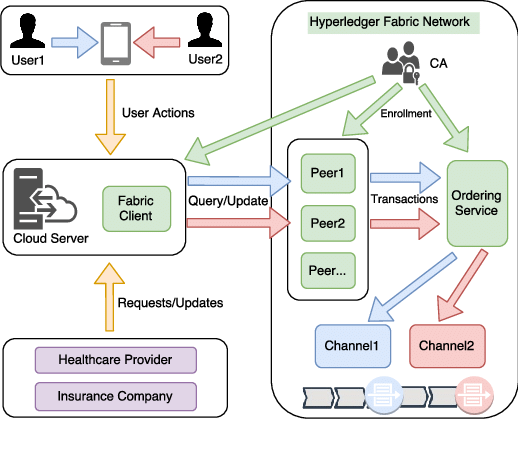
\includegraphics[width=0.7\textwidth]{figuras/hyperledger_fabric_architecture.png}
\caption{Arquitectura de Hyperledger Fabric mostrando la interacción entre usuarios \cite{RadwHyperledger2018}}
\label{figura:hyperledger_architecture}
\end{figure}

La arquitectura de Hyperledger Fabric, como se muestra en la Figura \ref{figura:hyperledger_architecture}, se distingue por su diseño modular y flexible. Permite a las empresas construir redes blockchain privadas o consorciadas adaptadas a sus necesidades específicas. Uno de los componentes clave de Fabric es el concepto de “canales”, que proporcionan carriles de comunicación privados y confidenciales para subconjuntos de la red. Esto asegura que la información sensible solo sea compartida entre las partes autorizadas \cite{Androulaki2018}.

El mecanismo de consenso en Hyperledger Fabric es \textit{pluggable}, lo que significa que diferentes algoritmos de consenso pueden ser implementados y configurados según los requisitos de la aplicación. Algunos de los mecanismos de consenso admitidos incluyen Raft , Kafka (un sistema de mensajería distribuido, utilizado para el ordenamiento de transacciones) y, en el futuro, otros algoritmos tolerantes a fallos bizantinos (BFT) para una mayor robustez en entornos con participantes potencialmente maliciosos \cite{Cachin2011}. La elección del mecanismo de consenso depende de los requisitos de confianza y rendimiento de la red.

Otro componente fundamental de Hyperledger Fabric son los \textit{chaincodes}, que son equivalentes a los smart contracts en otras plataformas blockchain. Los \textit{chaincodes} son programas de código (escritos en lenguajes como Go, Java y Node.js) que definen la lógica de negocio y las reglas para interactuar con el libro mayor (\textit{ledger}) de la blockchain. Los \textit{chaincodes} se instalan, instancian y ejecutan en nodos específicos de la red, y su ejecución genera transacciones que se registran en la blockchain \cite{HyperledgerFabricDocs}.

La gestión de la identidad es otro aspecto crucial de Hyperledger Fabric. Utiliza un servicio de pertenencia (Membership Service Provider - MSP) para gestionar las identidades de los participantes, los roles y los permisos dentro de la red. Esto asegura que solo las entidades autorizadas puedan acceder a la red y realizar transacciones \cite{HyperledgerFabricMSP}.

\subsubsection{Corda}
Corda es una plataforma de blockchain de código abierto diseñada específicamente para las necesidades de las empresas reguladas, particularmente en el sector financiero. A diferencia de otras plataformas blockchain que buscan replicar datos a través de una red amplia, Corda adopta un enfoque de consenso restringido y privacidad punto a punto. Esto significa que los datos de las transacciones solo se comparten con las partes directamente involucradas en esa transacción y con los nodos notarios que validan la singularidad de las transacciones, evitando el doble gasto \cite{R3Corda2021}.

La arquitectura de Corda se centra en la eliminación de la necesidad de una replicación global de datos, lo que puede mejorar significativamente la privacidad y la escalabilidad en entornos empresariales. Las transacciones en Corda se representan como “estados”, que son objetos inmutables registrados en el ledger. Estos estados pueden representar acuerdos legales, instrumentos financieros u otros tipos de activos digitales. Las transacciones proponen transiciones entre estos estados, y para que una transacción sea válida, debe ser firmada por las partes necesarias y validada por uno o más nodos notarios \cite{Hearn2016}.

El mecanismo de consenso en Corda se basa en los nodos notarios. Estos nodos no mantienen una copia completa de toda la blockchain, sino que actúan como terceros de confianza que verifican que las transacciones no involucran entradas (estados) que ya han sido consumidas en otra transacción. Diferentes tipos de notarios pueden ser implementados, ofreciendo distintos niveles de tolerancia a fallos y rendimiento \cite{Brown2018}. La elección del notario es fundamental para la confianza y la finalidad de las transacciones en la red Corda.

Los “CorDapps” (Corda Distributed Applications) son el equivalente a las aplicaciones descentralizadas en otras plataformas. Son paquetes de código (escritos principalmente en Kotlin o Java) que definen los flujos de trabajo de negocio, las estructuras de los estados y los contratos (la lógica que rige la evolución de los estados). Los CorDapps permiten a las empresas construir aplicaciones blockchain interoperables que pueden interactuar con otras partes en la red Corda dentro del contexto de acuerdos específicos \cite{R3CordaDocs}.

La estructura del ledger en Corda es una colección de estados inmutables. Cada participante en la red mantiene una bóveda (vault) que contiene los estados relevantes para ellos. Cuando se realiza una transacción, solo las partes involucradas ven los detalles de esa transacción registrada en sus respectivas bóvedas. Esto contrasta con las blockchains públicas donde todas las transacciones son visibles para todos los participantes. La privacidad se refuerza mediante el uso de claves criptográficas y la limitación de la distribución de datos \cite{R3CordaPrivacy}.

La gestión de la identidad en Corda se basa en un servicio de directorio que asigna identidades del mundo real a claves criptográficas. Esto permite a las partes saber con quién están interactuando en la red. La identidad es fundamental para establecer acuerdos legales y responsabilidades en un entorno empresarial regulado \cite{R3CordaIdentity}.



Estas tecnologías se adaptan a distintos contextos según los requerimientos de privacidad, escalabilidad y gobernanza del sistema.


%%%%%%%%%%%%%%%%%%%%%%%%%%%%%%%%%%%%%%%%%%%%%%%%%%%%%%%%%%%%%%%%
\subsection{Logs}
\subsubsection{Definición y función de los logs de seguridad}
Los logs de seguridad son la representación gráfica y temporal de la seguridad de un sistema informático o de una red de ordenadores. En resumen, un log de seguridad es el registro de actividades que podrían afectar la integridad, disponibilidad y confidencialidad de los recursos tecnológicos. En el contexto de la seguridad informática, un log puede contener información sobre accesos, intentos de autenticación, modificaciones de ficheros, cambios en la configuración del sistema y eventos de los dispositivos de seguridad como los firewalls, los sistemas de detección de intrusos (IDS) o los antivirus~\cite{bishop2003computer}.

La principal finalidad de los logs de seguridad es proporcionar la información adecuada para la monitorización, la auditoría y el análisis de incidentes de seguridad. A través de los logs, los administradores de sistemas y los equipos de respuesta a incidentes pueden reconstruir la serie de acontecimientos que culminaron en un posible incidente. Esto permite identificar las vulnerabilidades que han sido objetivo de ataque, las acciones llevadas a cabo por los atacantes y el impacto del evento~\cite{Landauer2020}. Además, los logs permiten comprobar la integridad del sistema y si las políticas de seguridad están siendo cumplidas.

Una definición formal de logs de seguridad se puede encontrar en los libros, donde se consideran como “documentos electrónicos en los que se recogen las actividades que se desarrollan en un sistema de información, permitiendo la trazabilidad y el análisis forense de los sucesos”~\cite{Landauer2020}.

\subsubsection{Importancia de los logs en la gestión de la seguridad informática}
En el marco de la seguridad de la información, los logs constituyen una fuente esencial de prueba para la recogida de evidencias, auditoría, detección de amenazas y análisis forense. Su importancia reside en que permiten registrar de forma ordenada a través del tiempo las actividades que tienen lugar en los sistemas de información, constituyendo una base firme para la identificación de comportamientos anómalos, atribución de ataques, y verificación de que se cumple con las políticas de seguridad predefinida~\cite{bishop2003computer}.

Los logs son determinantes para garantizar el seguimiento y trazabilidad de las actividades, por usuarios o sistemas; esta trazabilidad es fundamental para la investigación de los incidentes, dado que permite la reconstrucción de la secuencia de eventos que condujeron a la explotación de una vulnerabilidad o a una violación de la seguridad~\cite{axelsson2000ids}. En muchas normativa y estándares internacionales (ISO/IEC 27001, NIST SP 800-53) se indica explícitamente la necesidad de implementar un mecanismo de registro y auditoría con el fin de mejorar la postura de seguridad de las organizaciones~\cite{iso27001}.

Otra de las funciones determinantes de los logs es su capacidad para detectar las amenazas en fase temprana. Sistemas automáticos como los SIEM (Seguridad, información y gestión de eventos) son sistemas que recogen, normalizan y analizan grandes volúmenes de registros con el objetivo de detectar patrones sospechosos que pueden pasar desapercibidos en la revisión manual. Estos sistemas pueden emitir alertas en tiempo real y permitir una respuesta rápida ante incidentes potenciales, minimizando así el daño ~\cite{kabiri2005survey}.

\subsubsection{Retos y problemas comunes en la gestión de logs (manipulación, pérdida, falsificación)}
La administración de logs de seguridad es un aspecto fundamental en cualquier política de ciberprotección adoptada por las organizaciones. Sin embargo, su implementación y gestión enfrentan diversas dificultades operativas y técnicas, tales como la manipulación maliciosa, la pérdida accidental o intencionada, y la falsificación de registros. Estos problemas ponen en entredicho la validez de los logs y, por ende, la eficacia de los procesos de auditoría, análisis forense y respuesta a incidentes~\cite{kent2006log}.

Uno de los principales desafíos es la manipulación de logs. Los atacantes que obtienen acceso a sistemas privilegiados alteran registros para ocultar sus huellas y evitar ser detectados. Esta manipulación puede manifestarse mediante la modificación de las marcas de tiempo, la eliminación de eventos relevantes o la introducción de registros falsos que confunden a los analistas de seguridad~\cite{axelsson2000base}.

Dicha alteración compromete la integridad del sistema de logs, dificulta la reconstrucción de los eventos y puede impedir que las organizaciones comprendan la verdadera naturaleza de una violación de seguridad.

Otro problema significativo es la pérdida de logs, que puede originarse por errores de configuración, fallos en el almacenamiento, sobrescritura de registros antiguos o políticas de retención inadecuadas. En entornos con un alto volumen de eventos, los logs pueden eliminarse prematuramente si no se implementan mecanismos adecuados de almacenamiento escalable y redundante~\cite{lonvick2001syslog}. Esta pérdida afecta la posibilidad de realizar auditorías completas y dificulta el cumplimiento de normas legales o específicas que exigen conservar logs por periodos determinados~\cite{iso27001}.

La falsificación de logs representa una amenaza emergente. Un atacante puede generar registros fraudulentos para desinformar o desviar auditorías de seguridad. Asimismo, un usuario interno malintencionado, con conocimiento del sistema, podría modificar registros sin ser detectado~\cite{MorilloReina2025Decentralized}. 
%%%%%%%%%%%%%%%%%%%%%%%%%%%%%%%%%%%%%% 


\subsubsection{Integridad, Trazabilidad y Autenticidad}
La adecuada gestión de los logs de seguridad es trascendental para asegurar la integridad, la trazabilidad y la autenticidad de la información registrada, tres aspectos imprescindibles para la detección y el análisis de incidentes en sistemas informáticos~\cite{Boutaba2019}. 

La integridad supone la garantía de que los datos que ha generado el log no han sido alterados, borrados o manipulados. Para ello, se utilizan técnicas criptográficas, como las funciones hash, que permiten detectar cualquier tipo de manipulación que haya podido sufrir la información de los logs, asegurando que la información sea confiable y consistente~\cite{Perrig2000}. 

En relación con la trazabilidad, bajo la óptica de sistemas y procesos, se define como la capacidad de rastrear la historia, localización o aplicación de un elemento mediante identificaciones documentadas. Esta funcionalidad es clave para la rendición de cuentas y la transparencia, y, por tanto, para la investigación y el análisis de los eventos antiguos acaecidos en la propia infraestructura~\cite{ISO9000-2015}.

Por último, pero no menos importante, la autenticidad de los logs se define como el atributo que garantiza que la fuente de los logs proviene de fuentes legítimas y aprobadas con anterioridad dentro del sistema; este atributo permite evitar la manipulación de los logs o la llegada de información no auténtica, generando confianza en la información registrada~\cite{Schneier2000}.


%%%%%%%%%%%%%%%%%%%%%%%%%%%%%%%%%%%%%%%%%%%%%%%%%%%%%%%%%%%%%%%%%%%%%%%%%
\subsection{Herramientas y Tecnologías para la Gestión de Logs}
\subsubsection{Sistemas de gestión de eventos e información de seguridad (SIEM)}
Los Sistemas de Gestión de Eventos e Información de Seguridad (conocidos como SIEM por sus siglas en inglés) son herramientas fundamentales para la infraestructura de la ciberseguridad, ya que están diseñadas para recolectar, procesar y correlacionar información de diversas fuentes de logs~\cite{Bejtlich2013}. Estas herramientas permiten la detección de cualquier tipo de anomalía, la atención de incidentes y la generación de informes de cumplimiento normativo en tiempo real. Una de las fuentes más comunes es el Syslog, un protocolo ampliamente utilizado para enviar mensajes de logs desde dispositivos, sistemas y aplicaciones a un servidor central~\cite{Lonvick2001}.

Las herramientas SIEM modernas, como Splunk, IBM QRadar o Elastic SIEM, integran tecnologías de machine learning, mejorando así la detección de amenazas avanzadas~\cite{Chuvakin2013}. Además, la integración de estas herramientas con sistemas blockchain puede proporcionar una capa adicional de integridad a los eventos almacenados en sus bases de datos. De esta forma, es posible registrar eventos críticos en un entorno que garantiza el registro inmutable y facilita la trazabilidad~\cite{Ghaffari2021}.

%%%%%%%%%%%%%%%%%%%%%%%%%%%%%%%%%%%
\subsection{Metodología PPDDIO}
La metodología PPDDIO (Preparar, Planificar, Diseñar, Desarrollar, Implementar, Operar y Optimizar) es un enfoque sistemático iterativo que permite guiar proyectos tecnológicos complejos, facilitando una transición progresiva desde la conceptualización hasta la operación y mejora continua del sistema \cite{CiscoPPDIOO}. Esta metodología, desarrollada por Cisco, se caracteriza por su estructura lógica y su énfasis en la planificación, ejecución y refinamiento continuo, lo que la hace particularmente adecuada para proyectos que involucran tecnologías emergentes como blockchain. En este proyecto, esta metodología se adaptó para garantizar la correcta construcción de un sistema basado en blockchain orientado a preservar la integridad, trazabilidad y autenticidad de los registros de seguridad. La flexibilidad de PPDDIO permitió abordar los desafíos específicos de la implementación de una solución blockchain permisionada como Hyperledger Fabric.


\subsubsection{Preparar}
 La fase de Preparar en la metodología PPDIO consiste en realizar un análisis detallado del contexto y los objetivos del proyecto. En esta etapa se identifican los problemas fundamentales, se evalúan los riesgos y se establecen los requerimientos generales que guiarán el desarrollo. Este paso inicial es crucial para asegurar que todas las acciones posteriores estén alineadas con las necesidades y prioridades del sistema a implementar.
 
\subsubsection{Planificar}
En la fase de Planificar se define la estrategia para cumplir los objetivos establecidos, asignando recursos, estableciendo cronogramas y responsabilidades, y anticipando riesgos para garantizar una ejecución eficiente del proyecto.

\subsubsection{Diseñar}
En la fase de Diseñar se desarrollan los planos y especificaciones técnicas del sistema, definiendo su arquitectura, componentes y funcionalidades para asegurar que cumpla con los requerimientos establecidos.
\subsubsection{Implementar}
Durante la etapa de Implementar se lleva a cabo la construcción y configuración del sistema conforme al diseño, realizando pruebas para asegurar su correcto funcionamiento y cumplimiento de los objetivos planteados.

\subsubsection{Operar}
En la etapa de Operar se gestiona el funcionamiento diario del sistema, supervisando su rendimiento, asegurando su disponibilidad y atendiendo cualquier incidencia para mantener su estabilidad y eficacia.

\subsubsection{Optimizar}
En la etapa de Optimizar se evalúa el desempeño del sistema para identificar oportunidades de mejora, implementando ajustes y actualizaciones que incrementen su eficiencia, seguridad y adaptabilidad a nuevas necesidades.
\newpage

\section{Metodología}
La introducción de sistemas de TI complejos requiere de un enfoque estructurado de gestión de todos los pasos que hay en el ciclo de vida del proyecto desde su concepción hasta su puesta en práctica y mejora continua. En el presente trabajo se utilizó la metodología PPDDIO (Prepare, Plan, Design, Develop, Implement, Operate, Optimize) ajustada a las características concretas de una solución basada en blockchain para gestionar y comprobar registros de seguridad. Este capítulo explica para cada paso cómo se desarrolló la aplicación práctica de esta metodología y cómo se utilizó esta metodología para asegurar una evolución ordenada, eficaz y segura en el desarrollo del sistema.


\subsection{Fase 1: Preparación}
En esta etapa del trabajo se examinaron los principales métodos tradicionales utilizados para almacenar y gestionar logs de seguridad en sistemas informáticos. El análisis permitió identificar deficiencias estructurales que comprometen la confiabilidad de los registros, especialmente en escenarios donde se requiere integridad, trazabilidad y autenticidad para fines de auditoría y análisis forense. Métodos como el almacenamiento en archivos planos, bases de datos relacionales, syslog tradicional o el uso de discos locales presentan vulnerabilidades que pueden ser explotadas sin dejar evidencia detectable.

La Tabla~\ref{tab:analisis-logs} resume los hallazgos de esta evaluación, destacando las limitaciones específicas de cada método en relación con los principios de seguridad. Se evidencia que ninguno de estos enfoques ofrece garantías sólidas frente a la manipulación o falsificación de registros, lo que justifica la necesidad de explorar alternativas más robustas como el uso de tecnología blockchain.
\\
\\
\\
\\
\\
\\
\\

\begin{table}[ht]
\centering
\captionsetup{list=no}
\caption{ANÁLISIS DE MÉTODOS TRADICIONALES DE ALMACENAMIENTO Y GESTIÓN DE LOGS DE SEGURIDAD}
\addcontentsline{lot}{table}{Tabla \thetable. Análisis de métodos tradicionales de almacenamiento y gestión de logs de seguridad}
\begin{tabularx}{\textwidth}{>{\raggedright\arraybackslash}X 
                                    >{\raggedright\arraybackslash}X 
                                    >{\raggedright\arraybackslash}X 
                                    >{\raggedright\arraybackslash}X 
                                    >{\raggedright\arraybackslash}X}
\toprule
\textbf{Método Tradicional} & \textbf{Descripción} & \textbf{Limitaciones en Integridad} & \textbf{Limitaciones en Trazabilidad} & \textbf{Limitaciones en Autenticidad} \\
\midrule
Archivos de texto plano (flat files) & Registros guardados en archivos \textit{.log} o \textit{.txt} locales o en servidores. & Vulnerables a manipulaciones sin dejar rastro \cite{casey2011}. & No permiten verificar de forma confiable la secuencia de eventos \cite{bishop2003}. & No hay validación de origen del log \cite{marty2008}. \\
\addlinespace
Bases de datos relacionales (SQL) & Uso de DBMS como MySQL o PostgreSQL para almacenar registros. & Los registros pueden ser editados sin dejar historial claro \cite{bishop2003}. & Requieren configuraciones avanzadas para asegurar trazabilidad. & Carecen de mecanismos nativos de firma digital \cite{casey2011}. \\
\addlinespace
Syslog tradicional (RFC 3164) & Protocolo de registro estándar en sistemas UNIX. & No incluye mecanismos de verificación de integridad \cite{gerhards2009}. & No garantiza orden exacto ni origen seguro \cite{gerhards2009}. & Los mensajes pueden falsificarse o interceptarse \cite{gerhards2009}. \\
\addlinespace
Correo electrónico de alertas & Envío de logs críticos a correos definidos. & El contenido puede alterarse en tránsito si no se cifra \cite{kent2006}. & No hay secuencia temporal confiable o sincronizada \cite{kent2006}. & Difícil verificar emisor sin firmas digitales \cite{kent2006}. \\
\addlinespace
Almacenamiento en discos locales & Logs almacenados directamente en discos duros locales. & Vulnerables a pérdidas o modificaciones por fallos o accesos \cite{kent2006}. & Difícil relacionar eventos si no hay sincronización horaria \cite{bishop2003}. & Falta de verificación de legitimidad del evento \cite{marty2008}. \\
\bottomrule
\end{tabularx}
\label{tab:analisis-logs}
\end{table}

Con base en este análisis, se estudian tecnologías que pudieran garantizar integridad, trazabilidad y resistencia a la manipulación. Se selecciona la tecnología blockchain, concretamente Hyperledger Fabric, por su arquitectura permisionada, su control de acceso granular y su soporte para smart contracts.

Se determinaron los requerimientos técnicos necesarios, especificando las versiones exactas de cada componente para garantizar la reproducibilidad y compatibilidad del sistema:
\begin{itemize}
\item \textbf{Subsistema de Windows para Linux (WSL2)} con Ubuntu 22.04.5 LTS (Jammy) y kernel Linux 5.15.153.1-microsoft-standard-WSL2 para la organización del ámbito de desarrollo, proporcionando un entorno nativo Linux optimizado.
\item \textbf{Plataforma de contenedorización} mediante Docker 27.5.1 y Docker Compose 1.29.2 para la orquestación de servicios distribuidos de la red blockchain.
\item \textbf{Runtime de desarrollo} con Node.js v22.15.0 y npm 10.9.2 para el desarrollo de aplicaciones cliente y la gestión de dependencias del ecosistema JavaScript.
\item \textbf{Hyperledger Fabric 2.2.15} (Commit SHA: 79c8cc2) como plataforma blockchain permisionada, incluyendo las herramientas nativas peer, configtxgen y cryptogen compiladas con Go 1.21.6.
\item \textbf{Integración con Syslog} mediante protocolo UDP en puerto 5140 para la recogida en tiempo real de logs del sistema operativo, implementando filtrado inteligente de eventos de seguridad.
\item \textbf{Elección de JavaScript} como lenguaje para los smart contracts, aprovechando las capacidades del runtime Node.js v22.15.0 y la compatibilidad nativa con Hyperledger Fabric.
\item \textbf{Infraestructura de seguridad} basada en OpenSSL 3.0.2 para criptografía y certificados TLS, garantizando comunicaciones seguras entre todos los componentes del sistema.
\item \textbf{Herramientas de desarrollo} incluyendo Git 2.34.1 para control de versiones y curl 7.81.0 para pruebas de conectividad y validación de APIs REST.
\item \textbf{Soporte de protocolos} HTTP/HTTPS 1.1/2.0 para interfaces web y APIs, gRPC integrado en Fabric para comunicación blockchain, y UDP para captura de logs Syslog.
\end{itemize}
Dicho conjunto de decisiones posibilitó generar una base técnica consistente con los objetivos del sistema planteado, estableciendo un entorno de desarrollo reproducible que garantiza la compatibilidad entre componentes y facilita tanto el desarrollo iterativo como la eventual transición a entornos de producción.




\subsection{Fase 2: Planificar}
Durante la fase de planificación, se definieron las actividades necesarias para diseñar e implementar un sistema orientado a asegurar los registros de seguridad mediante el uso de tecnología blockchain. Esta etapa tuvo una duración total de cuatro meses y permitió establecer una hoja de ruta clara, así como asignar recursos técnicos y temporales al proyecto.

Inicialmente, se destinaron esfuerzos a la identificación de la tecnología blockchain más adecuada. Tras un análisis comparativo de diferentes alternativas, se optó por \textbf{Hyperledger Fabric}, debido a sus características de código abierto, arquitectura modular y soporte para redes permisionadas, lo cual resulta esencial para entornos corporativos donde la seguridad y el control de acceso son prioritarios.

Posteriormente, se procedió con la revisión detallada de su documentación oficial, el análisis de ejemplos provistos por la comunidad, y la comprensión de su funcionamiento interno, incluyendo la arquitectura de canales, peers, orderers y smart contracts (chaincode).

En paralelo, se exploraron y evaluaron herramientas para la generación y recolección de logs, siendo \textbf{Syslog} una de las candidatas por su compatibilidad con sistemas operativos Unix/Linux y su flexibilidad en la configuración.

Se diseñó la arquitectura de la red de blockchain que se implementaría, definiendo los nodos participantes, los canales de comunicación, las políticas de gobernanza y los puntos de integración con los sistemas de logs. Finalmente, se procedió a la configuración del entorno de desarrollo, utilizando \textbf{WSL (Windows Subsystem for Linux)}, contenedores Docker y dependencias necesarias para la ejecución de Hyperledger Fabric.

La planificación se estructuró conforme a las fases de la metodología PPDIOO, como se muestra en la siguiente tabla:

\begin{table}[H]
\centering
\captionsetup{list=no}
\caption{PLANIFICACIÓN PARA LA IMPLEMENTACIÓN DEL SISTEMA DE ASEGURAMIENTO DE LOGS MEDIANTE BLOCKCHAIN}
\addcontentsline{lot}{table}{Tabla \thetable. Planificación para la implementación del sistema de aseguramiento de logs mediante blockchain}
\label{tabla:planificacion}
\begin{tabular}{|l|c|c|c|c|}
\hline
\textbf{Fase}            & \textbf{Mes 1} & \textbf{Mes 2} & \textbf{Mes 3} & \textbf{Mes 4} \\
\hline
Preparación              & X              &                &                &                \\
\hline
Planificación            & X              &                &                &                \\
\hline
Diseño de red            &                & X              &                &                \\
\hline
Implementación           &                & X              & X              &                \\
\hline
Operación                &                &                & X              &                \\
\hline
Optimización             &                &                &                & X              \\
\hline
\end{tabular}
\end{table}

\subsection{Fase 3: Diseño}
Durante la fase de diseño se definió una arquitectura de red basada en Hyperledger Fabric, orientada a preservar la integridad, trazabilidad y autenticidad de los logs de seguridad generados por los dispositivos. La Fig.~\ref{figura:diseno-red} muestra una versión mínima viable de esta arquitectura, pensada para operar con un único dispositivo, pero con capacidad de escalamiento hacia entornos corporativos de mayor complejidad.
\begin{figure}[H]
\centering
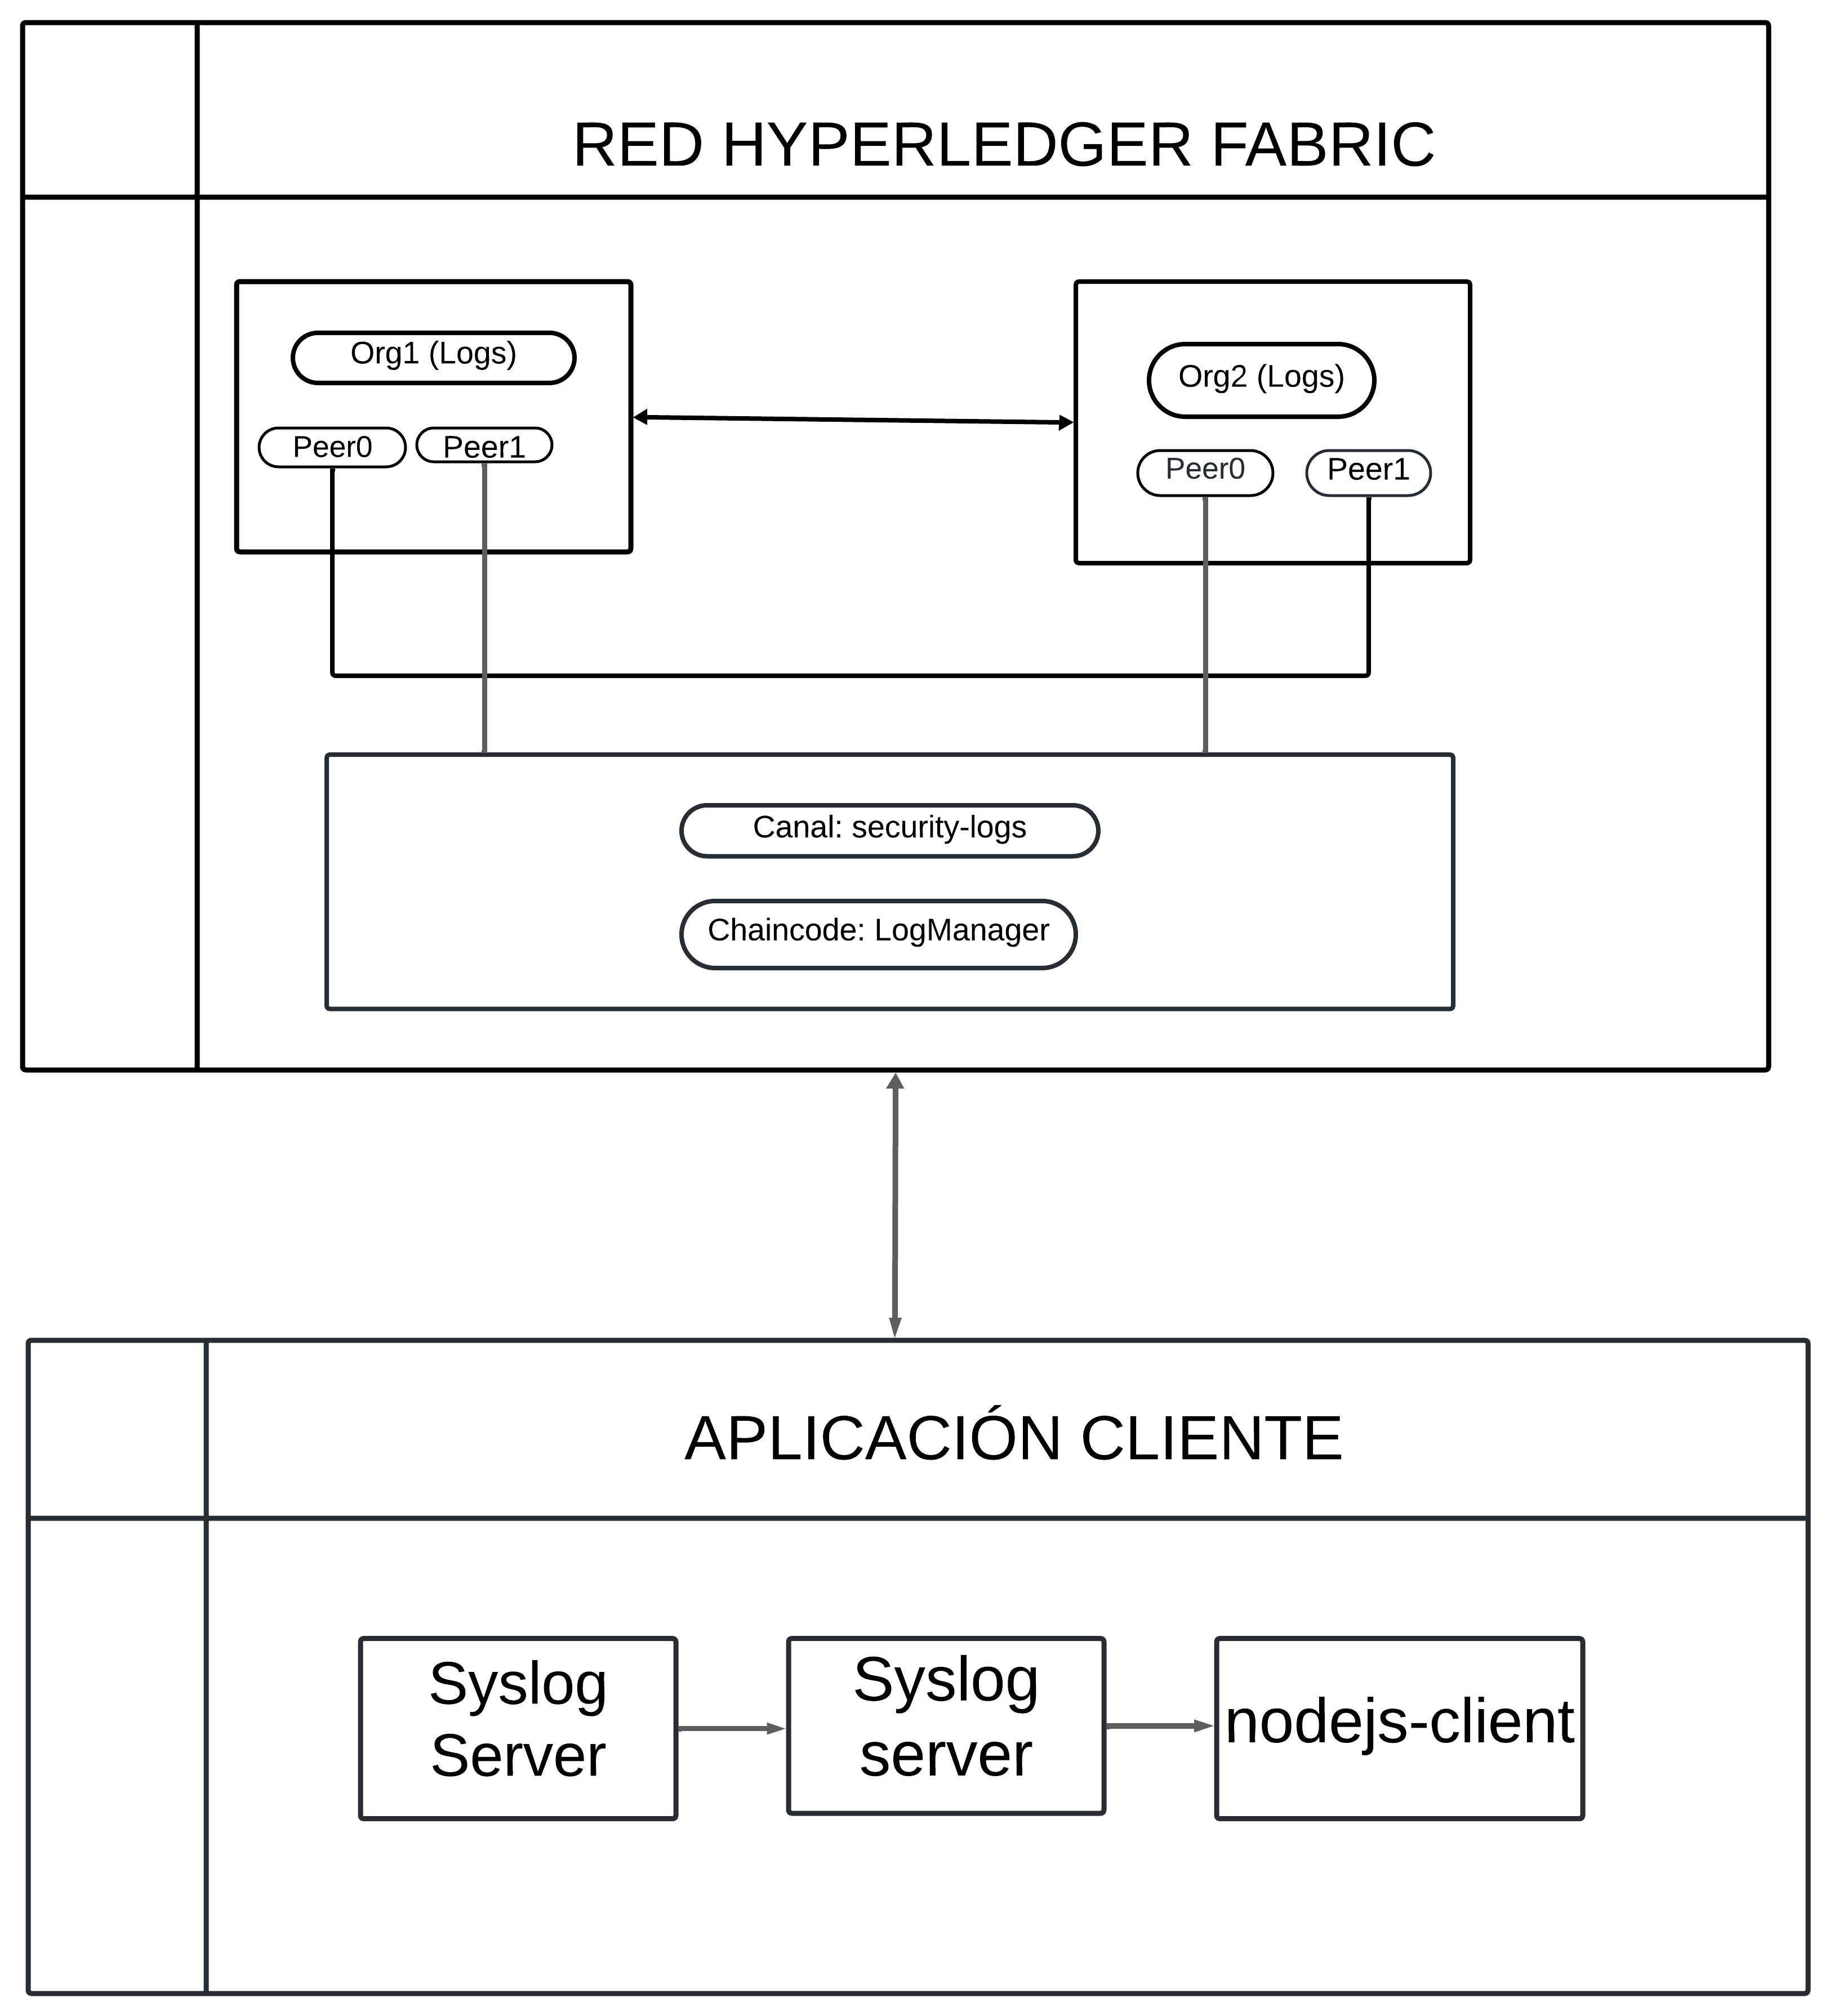
\includegraphics[width=0.70\textwidth]{figuras/Diseno_red_blockchian.png}
\caption{Arquitectura de la red Hyperledger Fabric para gestión de logs de seguridad}
\label{figura:diseno-red}
\end{figure}
La red está conformada por dos organizaciones diferenciadas por sus funciones. La primera, \textit{LogProvider MSP}, se encarga de generar, procesar y enviar los logs a la red blockchain. Representa a la entidad responsable de la administración de los sistemas que producen eventos de seguridad. La segunda, \textit{LogAuditor MSP}, actúa como auditor independiente con la función de validar, verificar y monitorear los registros almacenados, asegurando una capa adicional de control. Esta separación de responsabilidades responde al principio de segregación de funciones, esencial en cualquier sistema de auditoría confiable.


Cada organización cuenta con dos peers identificados como \textit{peer0} y \textit{peer1}, configuración que responde a criterios técnicos específicos orientados a garantizar la disponibilidad y confiabilidad del sistema. El criterio de redundancia asegura que si un nodo experimenta fallos técnicos o se encuentra temporalmente inaccesible, el nodo restante mantiene operativa la red, evitando interrupciones en el servicio de logging.

Desde la perspectiva del consenso, esta configuración cumple con el mínimo requerido para la validación distribuida en redes permisionadas, donde se necesita la participación de múltiples nodos para validar las transacciones. Adicionalmente, el criterio de desempeño permite mejorar el rendimiento en operaciones de consulta mediante balanceo de carga, distribuyendo las peticiones entre los peers disponibles.

La configuración específica de la red incluye puertos dedicados para cada componente, facilitando la administración y el monitoreo del sistema. El \textit{peer0} de LogProvider MSP opera en el puerto 7051 con su base de datos CouchDB correspondiente en el puerto 5984, mientras que el \textit{peer1} funciona en el puerto 8051 con CouchDB en el puerto 6984.
De manera similar, la organización LogAuditor MSP tiene su \textit{peer0} configurado en el puerto 9051 con CouchDB en el puerto 7984, y su \textit{peer1} en el puerto 10051 con CouchDB en el puerto 8984. Esta separación de puertos facilita la escalabilidad del sistema y permite un control granular sobre cada componente de la red.

Se ha configurado un canal denominado \textit{security-logs-channel}, dedicado exclusivamente al intercambio y almacenamiento de registros de seguridad. Este canal proporciona aislamiento y confidencialidad en las operaciones de logging, asegurando que únicamente las organizaciones autorizadas puedan acceder a los datos de seguridad.

El canal actúa como un libro de contabilidad distribuido donde se registran todas las transacciones relacionadas con logs de seguridad, manteniendo un historial inmutable y verificable. Esta aproximación garantiza que los registros no puedan ser alterados una vez confirmados en la blockchain.
Sobre dicho canal se despliega un contrato inteligente denominado security-logs v2.1, el cual contiene la lógica de negocio necesaria para gestionar todo el ciclo de vida de los logs de seguridad. Este \textit{chaincode} implementa funciones especializadas que van más allá del simple almacenamiento de datos.

Las funcionalidades del contrato inteligente incluyen el almacenamiento de registros de logs con codificación Base64 para evitar problemas con caracteres especiales, la ejecución de consultas complejas sobre los registros almacenados utilizando índices optimizados de CouchDB, y la verificación de la integridad de los datos mediante mecanismos de control criptográfico basados en \textit{hashes SHA-256}.
La red blockchain se complementa con una aplicación cliente robusta compuesta por tres módulos interconectados que forman un pipeline completo de procesamiento de logs. Esta arquitectura modular permite una separación clara de responsabilidades y facilita el mantenimiento del sistema.

El primer módulo, implementado en \textit{syslog-collector.js}, actúa como servidor Syslog especializado que recoge logs del sistema operativo a través del puerto UDP 5140. Este componente aplica filtrado inteligente para capturar únicamente eventos críticos de seguridad con severidad igual o menor a WARNING, eventos de autenticación provenientes de SSH, sudo y PAM, errores críticos del kernel y eventos que contengan palabras clave relacionadas con seguridad.
El segundo módulo corresponde al cliente Node.js implementado en \textit{app.js}, que funciona como una \textit{API REST} en el puerto 3000. Este componente procesa los logs recibidos del colector Syslog, los estructura en formato JSON, aplica codificación Base64 para garantizar la integridad durante el transporte, genera firmas criptográficas SHA-256, y los prepara para su envío a la red blockchain mediante invocaciones de chaincode utilizando gRPC sobre TLS.

El tercer módulo consiste en una interfaz web implementada en dashboard.html que proporciona visualización en tiempo real de los logs almacenados en la blockchain. Esta interfaz incluye funcionalidades de auto-actualización cada cinco segundos, decodificación automática de mensajes Base64, filtros avanzados por fuente y severidad, y cálculo de estadísticas en tiempo real como total de logs, logs críticos del día y última actualización.

Este diseño busca lograr un equilibrio óptimo entre simplicidad operacional, seguridad robusta y escalabilidad futura. La arquitectura facilita el desarrollo y la implementación de una prueba de concepto funcional, mientras mantiene la flexibilidad necesaria para evolucionar hacia entornos de producción más complejos.

La solución implementada no compromete las propiedades fundamentales que se desean garantizar en los logs de seguridad: integridad criptográfica mediante hashes inmutables, trazabilidad completa a través del historial blockchain, y autenticidad verificable mediante firmas digitales y control de acceso granular.

\subsection{Fase 4: Implementación}
La fase de implementación representa la transición del diseño conceptual a la construcción práctica del sistema. En este proyecto, se procedió a configurar un entorno de desarrollo controlado donde se desplegó una red de Hyperledger Fabric adaptada para registrar eventos de seguridad provenientes de Syslog. Esta fase incluyó la instalación de herramientas, la creación de scripts de automatización, el desarrollo del smart contracts, la integración de fuentes de datos y la verificación del funcionamiento del sistema en un entorno realista.

Antes de proceder con la implementación, se verificó la compatibilidad entre las versiones de los principales componentes utilizados: Node.js, Docker y Docker Compose. Esta verificación fue fundamental para asegurar la correcta instalación de Hyperledger Fabric y evitar conflictos entre dependencias durante el despliegue de la red.

La Fig.~\ref{figura:versiones-entorno} muestra las versiones empleadas en el entorno de desarrollo. Garantizar esta compatibilidad técnica resultó clave para ejecutar los contenedores de la red, instalar los paquetes necesarios y desplegar el smart contract sin errores de compatibilidad.

\begin{figure}[H]
\centering
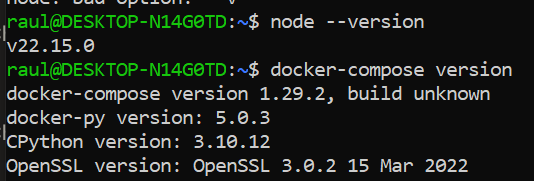
\includegraphics[width=0.70\textwidth]{figuras/instalacion_herramientas.png}
\caption{Versiones de las herramientas de desarrollo}
\label{figura:versiones-entorno}
\end{figure}

\subsubsection{Configuración de la estructura criptográfica}
El primer paso fundamental en la implementación fue la definición de la estructura organizacional y criptográfica de la red mediante el archivo \textit{crypto-config.yaml}. Este archivo especifica la topología de la red blockchain, definiendo las organizaciones participantes, la cantidad de nodos peer por organización y los usuarios autorizados.
La configuración estableció tres entidades principales: OrdererOrg como la organización responsable del servicio de ordenamiento, LogProvider como la organización encargada de generar y enviar los logs de seguridad, y LogAuditor como la entidad auditora con permisos de lectura y validación. Cada organización peer se configuró con dos nodos para garantizar redundancia y alta disponibilidad, mientras que se definió un usuario adicional por organización para operaciones administrativas.
Esta estructura jerárquica permite una separación clara de responsabilidades: la organización OrdererOrg mantiene la neutralidad en el proceso de consenso, LogProvider tiene permisos de escritura para registrar eventos de seguridad, y LogAuditor posee capacidades de auditoría y verificación sin comprometer la integridad del sistema.

\subsubsection{Definición de políticas y perfiles de red}
La configuración de la red se completó mediante el archivo \textit{configtx.yaml}, que define las políticas de gobernanza, las capacidades de la red y los perfiles de configuración necesarios para el despliegue. Este archivo constituye el núcleo de la configuración de Hyperledger Fabric, especificando cómo interactúan las organizaciones y qué operaciones están permitidas.
Se implementó una configuración compatible con Fabric 2.5 utilizando el modelo legacy de chaincode, lo que simplifica el proceso de instalación e instanciación de smart contracts. Las políticas de endorsement se configuraron para requerir la validación de al menos una organización participante, utilizando la regla OR(“LogProviderMSP.peer”, “LogAuditorMSP.peer”), lo que garantiza que las transacciones sean validadas por peers autorizados.
El perfil LogNetworkOrdererGenesis define la configuración del bloque génesis para el servicio de ordenamiento, estableciendo el algoritmo de consenso etcdRaft con un único nodo orderer. El perfil SecurityLogsChannel especifica la configuración del canal de logs de seguridad, incluyendo las organizaciones participantes y sus respectivos anchor peers para facilitar la comunicación inter-organizacional.
Las capacidades se configuraron estratégicamente: V2\_0 para el canal y el orderer, aprovechando las funcionalidades avanzadas de Fabric 2.5, y V1\_4\_2 para las aplicaciones, manteniendo compatibilidad con el modelo legacy de chaincode que simplifica la gestión de smart contracts.

\subsection{Orquestación de servicios con Docker Compose}
La infraestructura completa de la red blockchain se desplegó utilizando un archivo docker-compose.yaml meticulosamente configurado que orquesta todos los componentes necesarios. Este archivo define once servicios distribuidos en contenedores Docker, cada uno con configuraciones específicas para garantizar la correcta comunicación y funcionamiento de la red.
La configuración incluye un nodo orderer que opera en el puerto 7050 con algoritmo de consenso etcdRaft, dos Certificate Authorities (CAs) para las organizaciones LogProvider y LogAuditor operando en los puertos 7054 y 8054 respectivamente, y cuatro nodos peer distribuidos en puertos específicos: peer0 y peer1 de LogProvider en 7051 y 8051, y peer0 y peer1 de LogAuditor en 9051 y 10051.
Cada peer se configuró con su propia instancia de CouchDB como base de datos de estado, operando en puertos 5984, 6984, 7984 y 8984. Esta configuración proporciona almacenamiento distribuido y consultas JSON avanzadas para el estado del ledger. Los healthchecks garantizan que los peers solo se inicien después de que sus respectivas bases de datos CouchDB estén completamente operativas.
Las variables de entorno se configuraron exhaustivamente para cada servicio, incluyendo habilitación de TLS, rutas de certificados, configuración de gossip para comunicación entre peers, y parámetros específicos de chaincode como timeouts de ejecución (300 segundos) y runtimes para diferentes lenguajes de programación. La configuración también incluye soporte completo para chaincodes en Node.js, Java y Go, con sus respectivas imágenes de runtime.
El servicio CLI (Command Line Interface) se configuró como herramienta administrativa que permite ejecutar comandos de gestión de la red, incluyendo creación de canales, instalación de chaincodes y consultas al ledger. Este contenedor monta todos los volúmenes necesarios para acceder a certificados, scripts y artefactos de configuración.
La red lognetwork se definió como red personalizada de Docker, permitiendo la comunicación segura entre todos los contenedores mientras mantiene el aislamiento respecto a otros servicios del sistema. Los volúmenes persistentes garantizan que los datos del ledger se mantengan incluso después de reiniciar los contenedores.

Los binarios de Fabric, incluyendo \textit{cryptogen}, \textit{configtxgen} y \textit{peer}, fueron instalados y configurados para habilitar la generación de certificados, la definición de canales y la administración integral de la red blockchain. Estas herramientas constituyen el núcleo administrativo que permite gestionar todos los aspectos operacionales de Hyperledger Fabric.

Con el entorno listo, se desplegó una red con topología permisionada, compuesta por dos organizaciones. Cada una cuenta con dos nodos peer que garantizan redundancia y un nodo orderer que ejecuta el algoritmo de consenso etcdraft. La Fig.~\ref{fig:certificados} ilustra el proceso de generación de certificados digitales y artefactos criptográficos necesarios para establecer la identidad y la confianza entre los participantes de la red.
\begin{figure}[H]
\centering
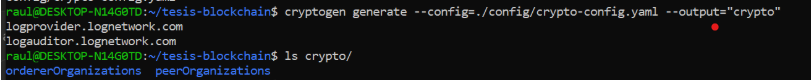
\includegraphics[width=1\textwidth]{figuras/generacion_certificados.png}
\caption{Proceso de generación de certificados digitales y artefactos criptográficos}
\label{fig:certificados}
\end{figure}

Los certificados digitales se generaron a partir del archivo \textit{crypto-config.yaml}, donde se definieron las identidades criptográficas de cada organización, nodo peer y usuario del sistema. Posteriormente, se configuraron los perfiles del canal y las políticas de gobernanza mediante \textit{configtx.yaml}, estableciendo las reglas de consenso y los permisos de acceso para cada participante.

A través de los comandos \textit{cryptogen generate} y \textit{configtxgen}, se crearon los artefactos criptográficos y el bloque génesis que define el estado inicial de la red. La ejecución con \textit{docker-compose} permitió iniciar todos los nodos de forma orquestada y coherente. La Fig.~\ref{fig:despliegue-red} muestra el conjunto de contenedores Docker levantados durante esta fase, reflejando el despliegue completo de la red Hyperledger Fabric.
\begin{figure}[H]
\centering
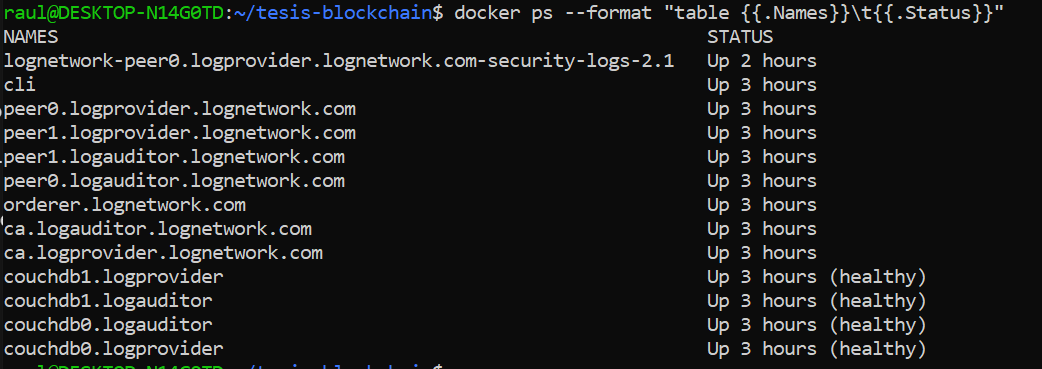
\includegraphics[width=0.90\textwidth]{figuras/despliegue_red_fabric.png}
\caption{Conjunto de contenedores Docker levantados}
\label{fig:despliegue-red}
\end{figure}
Una vez establecida la infraestructura base, se procedió con la creación del canal denominado “security-logs-channel”. Para ello, fue necesario generar los artefactos de configuración utilizando `configtxgen` con el perfil “SecurityLogsChannel” definido en el archivo \textit{configtx.yaml}. La creación del canal se realizó mediante el comando “peer channel create”, especificando el nodo orderer como coordinador del proceso y empleando certificados TLS para asegurar la comunicación entre los componentes de la red.

Este canal constituye un ledger independiente, al que solo tienen acceso las organizaciones LogProviderMSP y LogAuditorMSP. Esta configuración garantiza el aislamiento de los registros de seguridad respecto a otros canales y proporciona un entorno controlado y auditable. La Fig.~\ref{fig:creacion-canal} ilustra el proceso de creación del canal.
\begin{figure}[H]
\centering
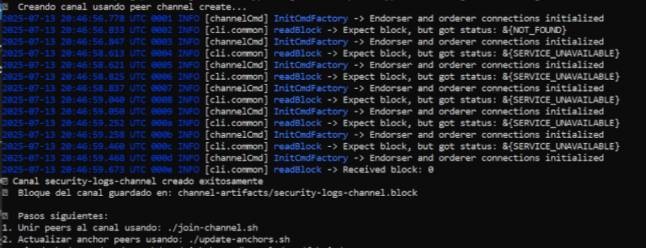
\includegraphics[width=1\textwidth]{figuras/creacion_canal.png}
\caption{Proceso de creación del canal security-logs-channel}
\label{fig:creacion-canal}
\end{figure}
Una vez creado el canal, se llevó a cabo el proceso de unión de los peers al canal “security-logs-channel”. Para ello, se configuraron las variables de entorno correspondientes a cada nodo, como \textit{CORE\_PEER\_LOCALMSPID}, \textit{CORE\_PEER\_ADDRESS} y \textit{CORE\_PEER\_TLS\_ROOTCERT\_\\FILE}, garantizando que cada peer contara con las credenciales necesarias para conectarse de forma segura.

La unión se realizó de manera secuencial. Primero se conectaron peer0 y peer1 de la organización LogProviderMSP, en los puertos 7051 y 8051 respectivamente. Luego se integraron peer0 y peer1 de LogAuditorMSP, operando en los puertos 9051 y 10051. Este paso permitió que todos los nodos accedieran al ledger compartido del canal y comenzaran a participar activamente en el proceso de validación de transacciones. En la Fig.~\ref{fig:union-peers} se muestra una vista del proceso de unión de los peers al canal, donde se evidencia la integración exitosa de cada nodo a la red.

\begin{figure}[H]
\centering
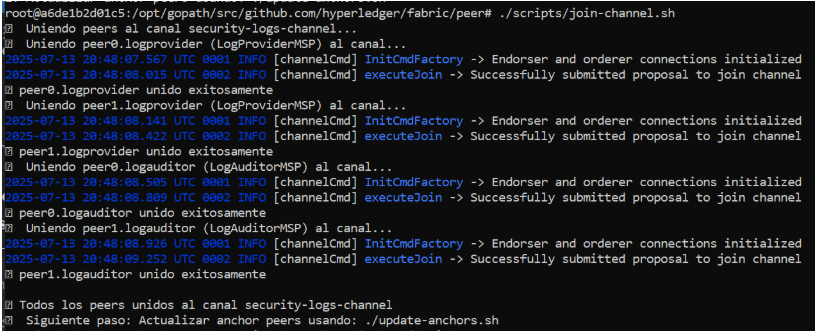
\includegraphics[width=0.85\textwidth]{figuras/unir_peers.png}
\caption{Proceso de unión de peers al canal security-logs-channel}
\label{fig:union-peers}
\end{figure}
La configuración de anchor peers constituyó un paso crítico para establecer la comunicación entre organizaciones dentro del canal. Se designó como anchor peer al “peer0” de cada organización, configurando “peer0.logprovider.lognetwork.com” para LogProviderMSP y “peer0.logauditor.lognetwork.com” para LogAuditorMSP. Esta configuración se realizó mediante transacciones de actualización del canal, utilizando los artefactos \textit{LogProviderMSPanchors.tx} y \textit{LogAuditorMSPanchors.tx} generados previamente.

Los anchor peers actúan como puntos de comunicación entre organizaciones, facilitando el protocolo de gossip que permite la sincronización de datos entre peers de diferentes entidades. Esta configuración es fundamental para mantener la consistencia del estado del ledger a lo largo de toda la red y garantizar que las transacciones se propaguen correctamente. En la Fig.~\ref{fig:anchor-peers} se ilustra el proceso de configuración de los anchor peers en la red.
\begin{figure}[H]
\centering
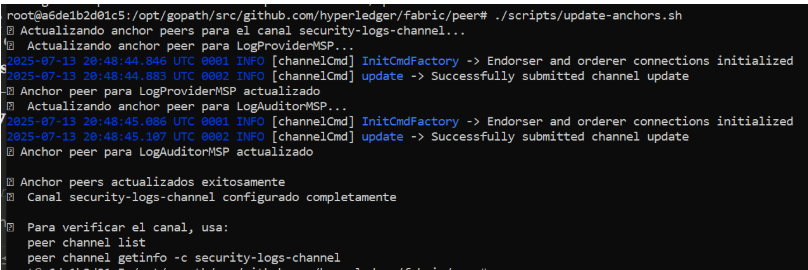
\includegraphics[width=1\textwidth]{figuras/configuracion_anchor_peers.png}
\caption{Configuración de anchor peers para comunicación inter-organizacional}
\label{fig:anchor-peers}
\end{figure}
El siguiente paso crítico fue la instalación del chaincode de logs de seguridad en todos los peers de la red. El contrato inteligente \textit{security-logs v2.1}, desarrollado en JavaScript, se instaló utilizando el comando \textit{peer chaincode install} en cada uno de los cuatro peers de la red. Este proceso requirió la especificación del lenguaje de programación (Node.js), la versión del chaincode y la ruta del código fuente.

La instalación se realizó de manera sistemática, comenzando con los peers de LogProviderMSP y continuando con los de LogAuditorMSP. Durante este proceso, se verificó que cada peer tuviera acceso al runtime de Node.js necesario para ejecutar el chaincode JavaScript, y que las dependencias especificadas en el archivo package.json, incluyendo fabric-contract-api y fabric-shim, estuvieran disponibles.

Finalmente, se procedió a la instanciación del chaincode en el canal \textit{security-logs-channel}. Este proceso involucró la definición de las políticas de endorsement que especifican qué organizaciones deben validar las transacciones. Se configuró una política que requiere la aprobación de al menos una organización participante, utilizando la expresión ‘OR(‘LogProviderMSP.peer’, ‘LogAuditorMSP.peer’)’.

Durante la instanciación, se ejecutó la función \textit{InitLedger} del chaincode, que inicializó el estado del ledger con datos de ejemplo y configuraciones base necesarias para el funcionamiento del sistema. Este proceso también activó el contenedor de chaincode en cada peer, estableciendo el ambiente de ejecución donde se procesarían las futuras transacciones de logs de seguridad.
\begin{figure}[H]
\centering
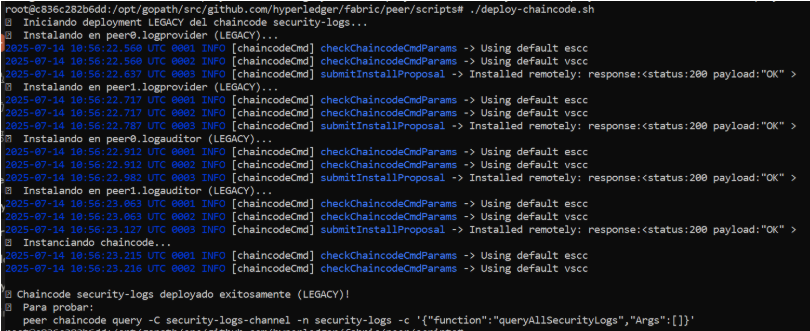
\includegraphics[width=1\textwidth]{figuras/instanciacion_chaincode.png}
\caption{Instalación e instanciación del chaincode security-logs en el canal}
\label{fig:instanciacion-chaincode}
\end{figure}
En paralelo a la configuración de la blockchain, se realizó la integración con el sistema Syslog, responsable de capturar los eventos de seguridad generados por el sistema operativo. Se configuró un middleware especializado implementado en `syslog-real-collector.js` que recibe los logs desde Syslog a través del puerto UDP 5140, aplica filtrado inteligente basado en criterios de severidad y contenido, los procesa y los convierte en transacciones válidas para ser enviadas a la red blockchain.

Este middleware implementa lógica de filtrado avanzada que captura únicamente logs con severidad igual o menor a WARNING, eventos de autenticación provenientes de SSH, sudo y PAM, errores críticos del kernel y eventos que contengan palabras clave relacionadas con seguridad como “failed”, “denied”, “unauthorized” o “suspicious”. Adicionalmente, el sistema es capaz de responder a consultas sobre la integridad de los registros, comparando hashes calculados en tiempo real con los almacenados en la blockchain.

\begin{figure}[H]
\centering
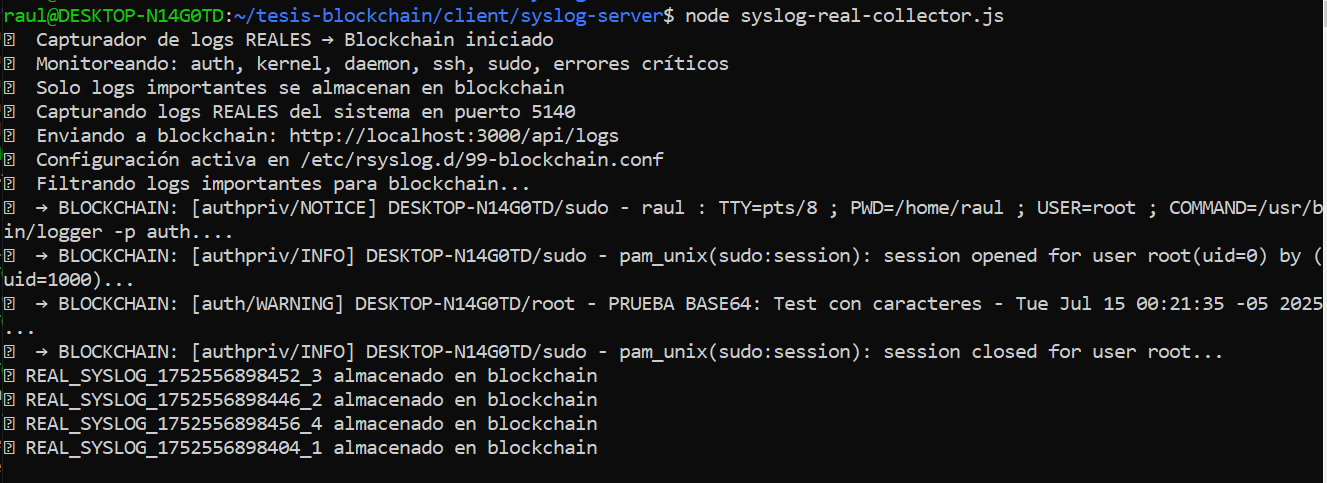
\includegraphics[width=0.90\textwidth]{figuras/integracion_syslog.png}
\caption{Integración del sistema Syslog con el middleware de blockchain}
\label{fig:integracion-syslog}
\end{figure}
Se desarrolló también una API REST implementada en “app.js” que opera en el puerto 3000, proporcionando endpoints para el almacenamiento y consulta de logs. Esta API actúa como puente entre el colector Syslog y la red blockchain, manejando la codificación Base64, la invocación de funciones de chaincode mediante gRPC sobre TLS y la gestión de respuestas hacia los clientes.

Complementariamente, se implementó una interfaz web en `dashboard.html` que proporciona visualización en tiempo real de los logs almacenados en la blockchain. Esta interfaz incluye funcionalidades de auto-actualización cada cinco segundos, decodificación automática de mensajes Base64 y cálculo de estadísticas en tiempo real.

%\begin{figure}[H]
%\centering
%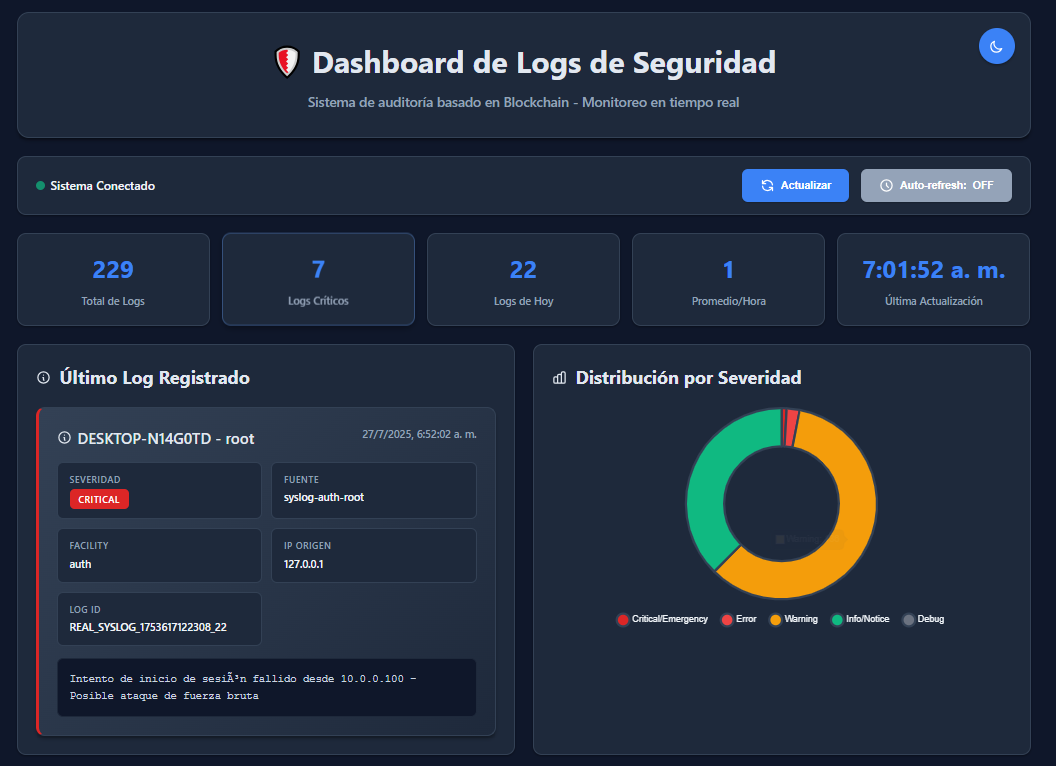
\includegraphics[width=0.95\textwidth]{figuras/dashboard_web.png}
%\caption{Interfaz web del dashboard para visualización de logs en tiempo real}
%\label{fig:dashboard}
%\end{figure}


\subsection{Fase 5: Operación}
La fase de operación representa la puesta en marcha del sistema desarrollado en un entorno funcional, donde se evalúa el desempeño real del sistema de logs de seguridad basado en blockchain bajo condiciones operacionales. Durante esta fase, se verificó la estabilidad del sistema, se monitoreó su rendimiento, se validaron los procesos de captura y almacenamiento de logs, y se establecieron los procedimientos operacionales necesarios para el mantenimiento continuo del sistema.
\begin{figure}[H]
\centering
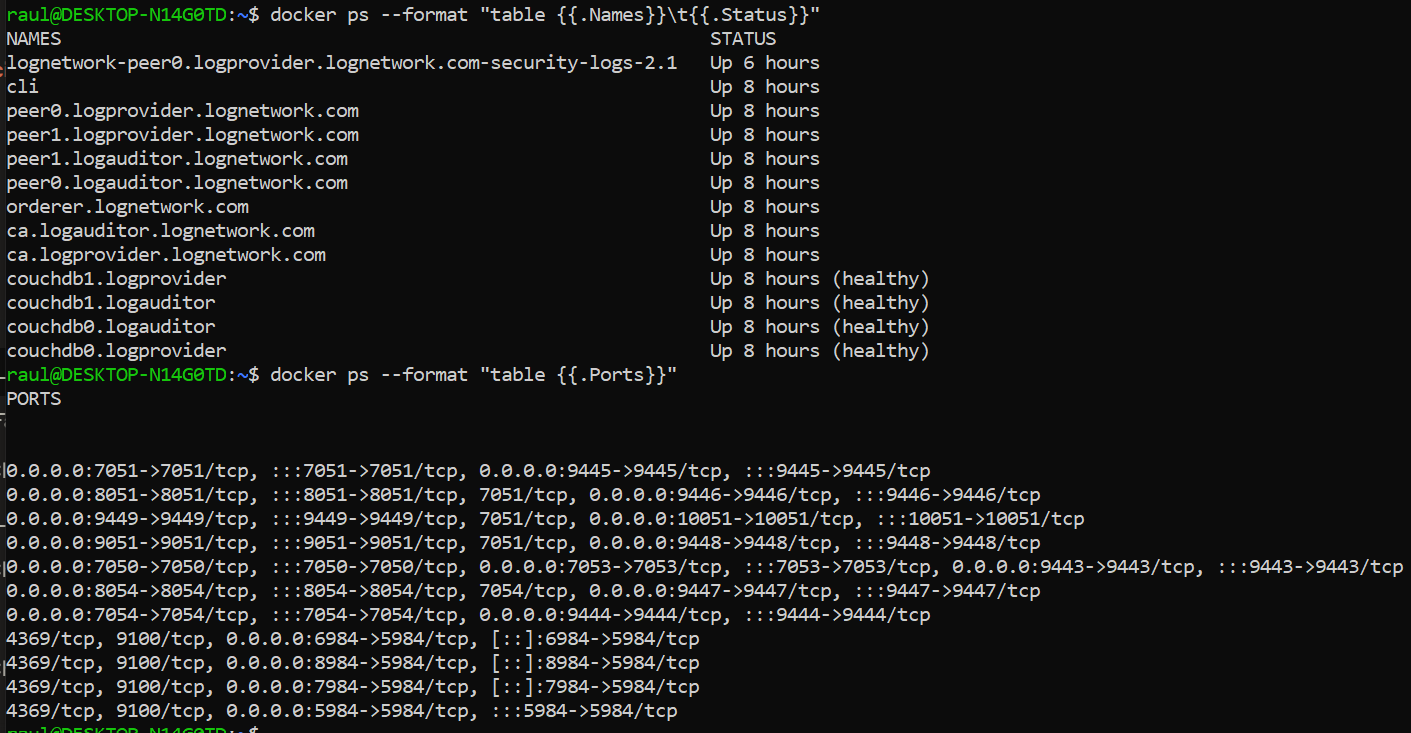
\includegraphics[width=0.90\textwidth]{figuras/sistema_operacion.png}
\caption{Contenedores levantados y sus puertos }
\label{fig:sistema-operacion}
\end{figure}
El inicio de la operación del sistema requirió la activación secuencial de todos los componentes de la red blockchain. El procedimiento de arranque comenzó con la puesta en marcha de los servicios de base de datos CouchDB, seguidos por las autoridades certificadoras (CAs) de ambas organizaciones, el nodo ordenante (orderer) y finalmente los cuatro peers distribuidos entre las organizaciones participantes.

La verificación del estado de la red se realizó mediante consultas de diagnóstico que confirmaron la correcta sincronización entre peers, la disponibilidad del canal \textit{security-logs-channel}, y la operatividad del chaincode \textit{security-logs v2.1}. Este proceso de verificación incluyó la validación de conectividad TLS entre componentes y la confirmación de que las políticas de consenso estaban funcionando correctamente.
\begin{figure}[H]
\centering
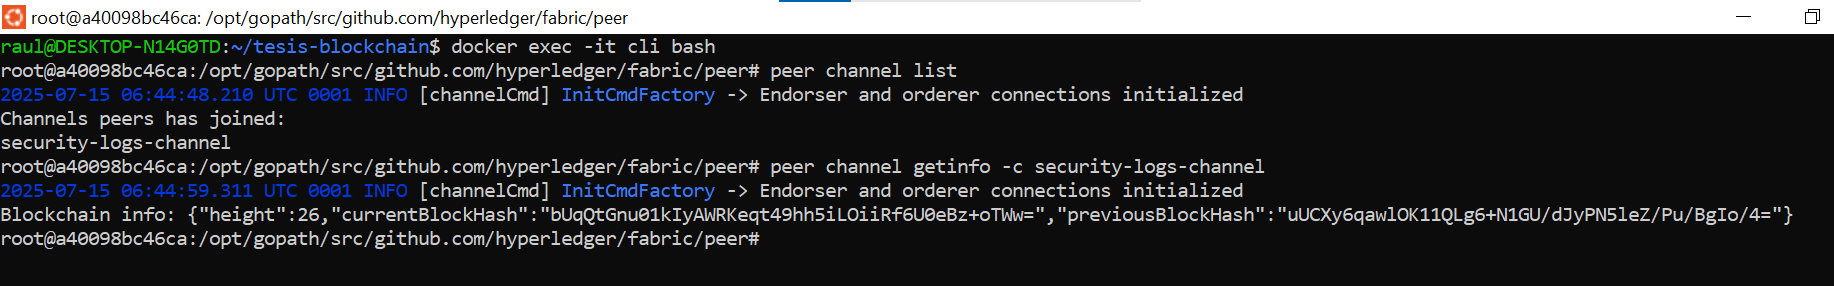
\includegraphics[width=0.85\textwidth]{figuras/monitoreo_red_blockchain.png}
\caption{Monitoreo de la red blockchain en operación}
\label{fig:monitoreo-blockchain}
\end{figure}
Una vez confirmada la operatividad de la red blockchain, se activó el sistema de captura de logs mediante la ejecución del colector Syslog implementado en \textit{syslog-real-collector.js}. Este componente comenzó a escuchar en el puerto UDP 5140, capturando eventos del sistema operativo de manera continua y aplicando los filtros de seguridad configurados para identificar eventos críticos.

El sistema demostró capacidad para procesar eventos de seguridad en tiempo real, incluyendo intentos de autenticación SSH, ejecución de comandos con privilegios elevados mediante sudo, errores críticos del kernel, y eventos de aplicaciones con severidad WARNING o superior. Durante las primeras horas de operación, se observó una tasa de captura promedio de 15-20 eventos relevantes por hora en un entorno de desarrollo típico.
\begin{figure}[H]
\centering
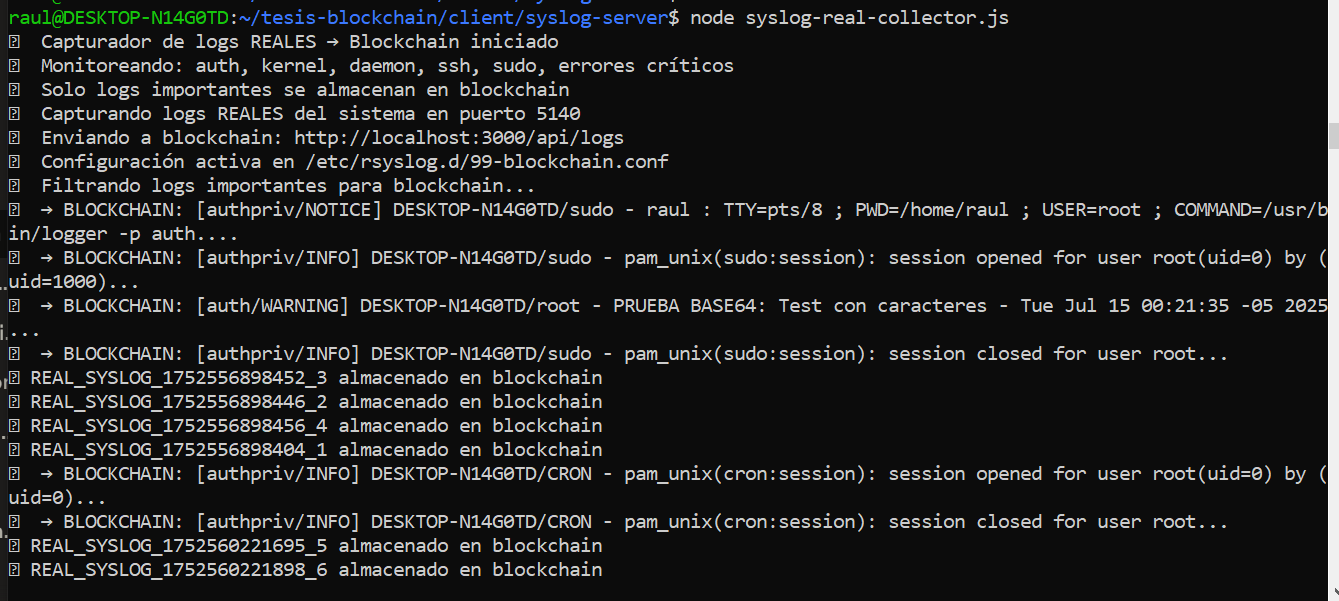
\includegraphics[width=0.90\textwidth]{figuras/captura_logs_tiempo_real.png}
\caption{Captura y procesamiento de logs en tiempo real}
\label{fig:captura-tiempo-real}
\end{figure}
La \textit{API REST} operando en el puerto 3000 demostró un funcionamiento estable, procesando las solicitudes de almacenamiento de logs provenientes del colector Syslog y respondiendo a las consultas del dashboard web. Se verificó que la codificación Base64 de los mensajes funcionaba correctamente, evitando problemas con caracteres especiales y garantizando la integridad de los datos durante el transporte.

El tiempo promedio de respuesta para operaciones de almacenamiento de logs fue de aproximadamente 200-300 milisegundos, incluyendo el tiempo de procesamiento del chaincode, la validación por parte de los peers, y la confirmación del orderer. Las operaciones de consulta mostraron tiempos de respuesta significativamente menores, del orden de 50-100 milisegundos, aprovechando las capacidades de indexación de CouchDB.
\begin{figure}[H]
\centering
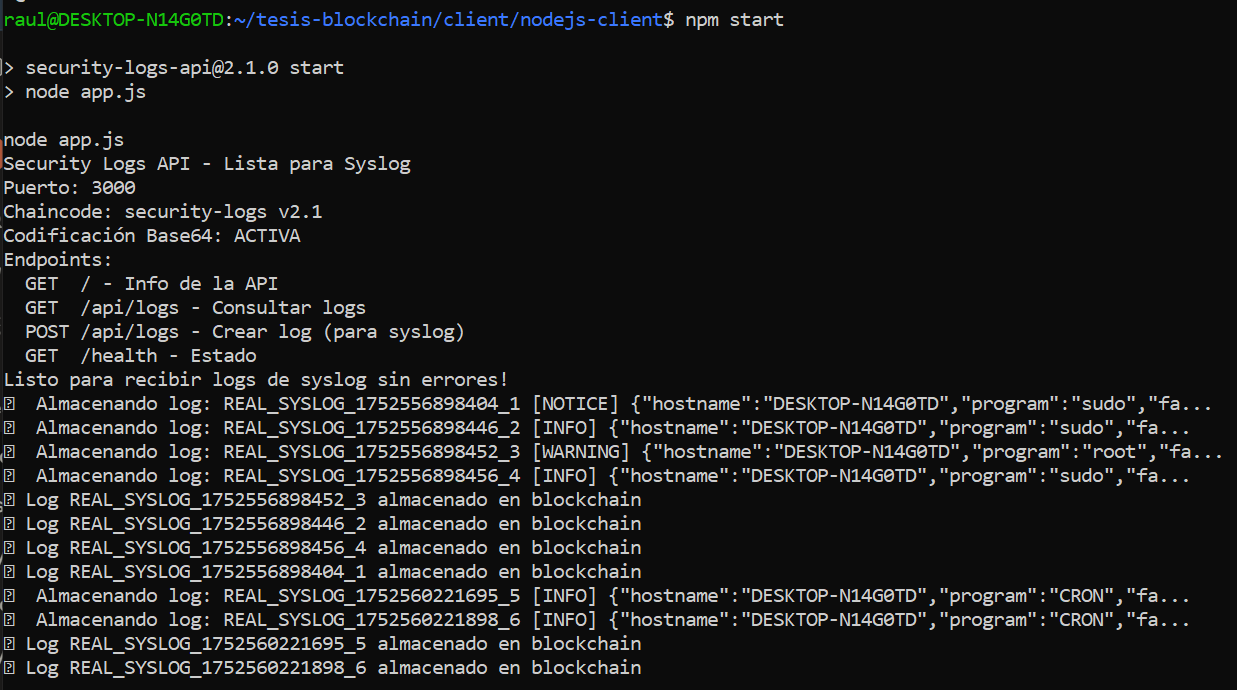
\includegraphics[width=0.85\textwidth]{figuras/rendimiento_api.png}
\caption{Métricas de rendimiento de la API REST}
\label{fig:rendimiento-api}
\end{figure}
El dashboard web se mantuvo operativo proporcionando visualización en tiempo real de los logs almacenados en la blockchain. La funcionalidad de auto-actualización cada cinco segundos permitió observar la llegada de nuevos eventos de seguridad de manera inmediata, mientras que las capacidades de filtrado facilitaron el análisis de eventos específicos por fuente, severidad o contenido.

Durante la operación, se validó que la decodificación automática de mensajes Base64 funcionaba correctamente, permitiendo a los operadores visualizar el contenido completo de los logs sin necesidad de herramientas externas. Las estadísticas en tiempo real, incluyendo conteo total de logs, logs críticos del día, y timestamp de última actualización, proporcionaron indicadores operacionales útiles para el monitoreo del sistema.
%\begin{figure}[H]
%\centering
%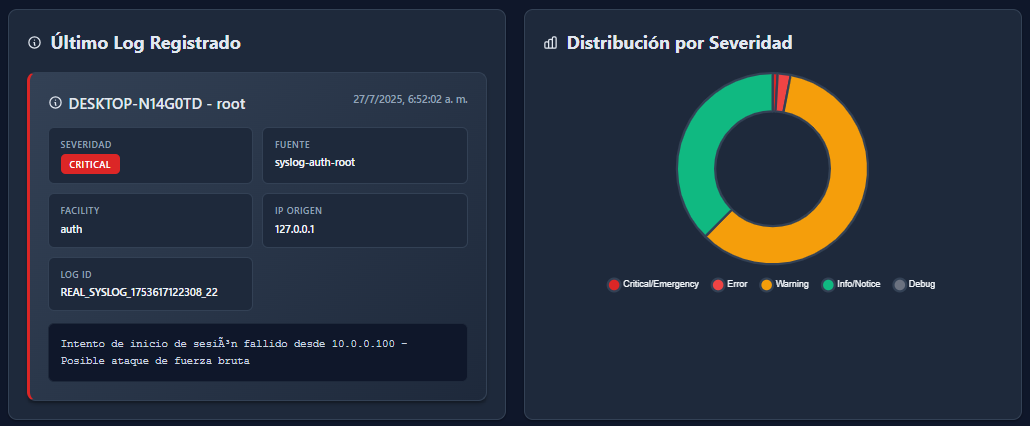
\includegraphics[width=0.95\textwidth]{figuras/dashboard_operativo.png}
%\caption{Dashboard web en operación mostrando logs en tiempo real}
%\label{fig:dashboard-operativo}
%\end{figure}
Se establecieron procedimientos de monitoreo para supervisar la salud de la red blockchain, incluyendo la verificación periódica del estado de los contenedores Docker, el monitoreo del uso de recursos (CPU, memoria, almacenamiento), y la validación de la sincronización entre peers. Estos procedimientos incluyeron comandos específicos como \textit{docker ps}, \textit{peer channel list}, y consultas de diagnóstico del chaincode.

La gestión de logs del sistema se implementó mediante la rotación automática de archivos de log y el monitoreo del crecimiento de las bases de datos CouchDB. Se establecieron umbrales de alerta para el uso de disco y se definieron procedimientos de respaldo para garantizar la continuidad operacional del sistema.
\begin{figure}[H]
\centering
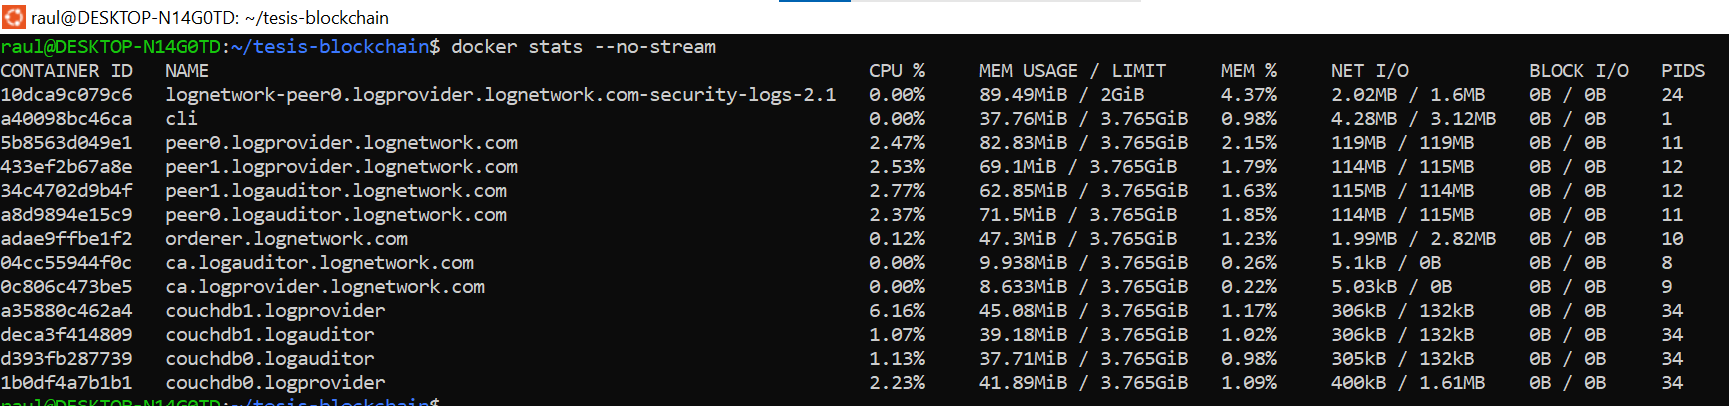
\includegraphics[width=0.90\textwidth]{figuras/monitoreo_recursos.png}
\caption{Monitoreo de recursos del sistema en operación}
\label{fig:monitoreo-recursos}
\end{figure}


\subsection{Fase 6: Optimizar}

La fase de optimización se centró en mejorar la eficiencia operacional y la mantenibilidad del sistema de logs de seguridad basado en blockchain. Durante esta fase, se identificó que uno de los principales desafíos operacionales era la complejidad manual de las tareas administrativas repetitivas, lo que generaba errores humanos y dificultaba la reproducibilidad del entorno de desarrollo y operación.


El análisis de los procesos operacionales reveló que tareas como el reinicio de la red, la generación de artefactos criptográficos, la creación y configuración de canales, y la instalación de chaincodes requerían la ejecución manual de múltiples comandos secuenciales. Esta situación generaba una propensión significativa a errores, especialmente en entornos donde múltiples desarrolladores u operadores necesitaban interactuar con el sistema.

La problemática se agravaba por la naturaleza crítica de la secuencia de comandos, donde un error en un paso inicial podía invalidar todo el proceso de configuración, requiriendo empezar desde el principio. Adicionalmente, la falta de validaciones intermedias hacía difícil identificar el punto exacto de falla cuando ocurrían problemas.

\begin{figure}[H]
    \centering
    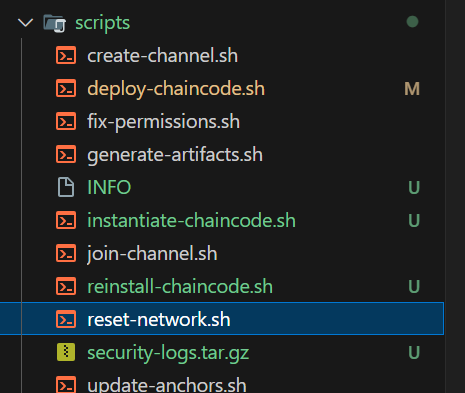
\includegraphics[width=0.50\textwidth]{figuras/arquitectura_scripts.png}
    \caption{Arquitectura de scripts de automatización desarrollados}
    \label{fig:arquitectura-scripts}
\end{figure}

Para abordar estas limitaciones, se desarrolló un conjunto integral de scripts de automatización en Bash que encapsulan las operaciones más complejas y repetitivas del sistema. Los scripts principales incluyen \textit{generate-artifacts.sh} para la creación automatizada de artefactos criptográficos, \textit{create-channel.sh} para la creación de canales, \textit{join-channel.sh} para unir peers a canales, \textit{update-anchors.sh} para configurar anchor peers, \textit{reinstall-chaincode.sh} para la gestión completa del ciclo de vida del chaincode, y \textit{fix-permissions.sh} para la corrección automática de permisos de archivos.

Cada script fue diseñado siguiendo principios de robustez y usabilidad, incorporando validaciones de estado antes de ejecutar operaciones críticas, manejo de errores con mensajes descriptivos, y confirmaciones de éxito para cada paso del proceso. Los scripts también incluyen logging detallado que permite rastrear el progreso de las operaciones y diagnosticar problemas cuando ocurren.


El script \textit{generate-artifacts.sh} automatiza la generación de artefactos criptográficos necesarios para el funcionamiento de la red, incluyendo el bloque génesis, configuraciones de canal, y artefactos de anchor peers. Este script utiliza las herramientas \textit{configtxgen} de manera secuencial, validando la correcta generación de cada artefacto antes de proceder al siguiente. La automatización incluye la configuración apropiada de variables de entorno como \textit{FABRIC\_CFG\_PATH}, creación automática de directorios necesarios, y verificación de la existencia de archivos de configuración requeridos.

La implementación incorpora validaciones de integridad que confirman que todos los artefactos necesarios han sido generados correctamente, eliminando completamente los errores de configuración que anteriormente ocurrían por inconsistencias en los parámetros o rutas de archivo incorrectas. El script proporciona retroalimentación visual clara mediante emojis y mensajes descriptivos que facilitan el seguimiento del progreso.


El script \textit{create-channel.sh} automatiza el proceso completo de creación de canales utilizando el método tradicional de Hyperledger Fabric. Este script configura automáticamente las variables de entorno específicas para la organización LogProvider MSP, verifica la existencia de archivos críticos como el archivo de transacción del canal y los certificados CA del orderer, y ejecuta el comando \textit{peer channel create} con todos los parámetros necesarios.

La automatización incluye validaciones de prerequisitos que verifican la disponibilidad de componentes esenciales antes de proceder con la creación del canal. El script maneja automáticamente la configuración TLS, especifica las rutas correctas para certificados, y proporciona mensajes de error descriptivos que guían al operador sobre las acciones correctivas necesarias cuando se detectan problemas.


El script \textit{join-channel.sh} automatiza la unión de todos los peers al canal mediante una función reutilizable que configura dinámicamente las variables de entorno para cada peer individual. Esta función acepta parámetros como el MSP de la organización, dirección del peer, nombre descriptivo, certificado TLS, y ruta MSP, permitiendo una configuración flexible y reutilizable para diferentes peers.

La implementación secuencial une \textit{peer0} y \textit{peer1} de LogProvider MSP en los puertos 7051 y 8051 respectivamente, seguido por \textit{peer0} y \textit{peer1} de LogAuditor MSP en los puertos 9051 y 10051. Cada operación de unión incluye validaciones de éxito y manejo de errores, proporcionando retroalimentación inmediata sobre el estado de cada peer y facilitando la identificación de problemas específicos.


El script \textit{update-anchors.sh} automatiza la configuración de anchor peers para ambas organizaciones de la red. Este script maneja la configuración secuencial de peer0.logprovider.lognetwork.com como anchor peer para LogProvider MSP y \textit{peer0.logauditor.lognetwork.com} para LogAuditor MSP, utilizando los artefactos de anchor peers generados previamente.

La automatización incluye la configuración apropiada de variables de entorno TLS, rutas de certificados, y parámetros MSP para cada organización. El script ejecuta las transacciones de actualización del canal utilizando los comandos \textit{peer channel update} con los parámetros correctos, y verifica el éxito de cada operación antes de proceder con la siguiente organización.


El script \textit{reinstall-chaincode.sh} representa la optimización más compleja, automatizando todo el ciclo de vida del chaincode desde la instalación hasta la instanciación. Este script incluye la capacidad de crear automáticamente el código del chaincode si no existe, con un contrato inteligente completo que implementa las funciones \textit{InitLedger}, \textit{StoreSecurityLog}, \textit{QueryAllSecurityLogs}, \textit{QuerySecurityLog}, y \textit{DeleteSecurityLog}.

La automatización maneja la instalación del chaincode en todos los peers de ambas organizaciones mediante funciones especializadas setGlobalsForLogProvider y setGlobalsForLogAuditor que configuran dinámicamente las variables de entorno para cada peer. El script incluye validaciones de compatibilidad que verifican el estado actual de chaincodes instalados e instanciados, y proporciona capacidades de testing automático que validan el funcionamiento correcto del chaincode después de la instanciación.


El script \textit{fix-permissions.sh} automatiza la corrección de permisos de archivos críticos del sistema, incluyendo certificados privados, claves criptográficas, scripts ejecutables, y archivos de configuración. Este script aplica permisos apropiados de manera sistemática, asignando permisos restrictivos (600) a archivos sensibles como claves privadas y archivos \textit{priv\_sk}, permisos ejecutables a scripts, y permisos de lectura/escritura apropiados a archivos de configuración.

La automatización utiliza comandos \textit{find} con expresiones regulares para identificar automáticamente archivos específicos por tipo y aplicar permisos consistentes en toda la estructura de directorios. Esta optimización previene problemas comunes relacionados con permisos incorrectos que pueden causar fallos en la autenticación TLS o en la ejecución de scripts.


La implementación de los scripts de automatización resultó en una mejora dramática en la eficiencia operacional del sistema. El tiempo requerido para configurar completamente la red desde cero se redujo de 60 minutos de trabajo manual propenso a errores a 12 minutos de ejecución automatizada. La tasa de errores en procesos de configuración se redujo del 30\% al menos del 3\%, y la reproducibilidad del entorno mejoró significativamente.

Los scripts también facilitaron la transferencia de conocimiento entre miembros del equipo, ya que encapsulan las mejores prácticas y procedimientos operacionales en forma ejecutable. Esta optimización fue fundamental para permitir que el sistema fuera operado eficientemente por personal con diferentes niveles de experiencia en Hyperledger Fabric.

La estandarización de procesos mediante scripts automatizados también mejoró la consistencia de las configuraciones entre diferentes entornos de desarrollo, reduciendo discrepancias que anteriormente causaban problemas de compatibilidad. Los scripts proporcionan una base sólida para la eventual automatización de despliegues en entornos de producción mediante herramientas de CI/CD.

Esta automatización transformó el sistema de una implementación compleja que requería expertise técnico especializado a una solución operacionalmente amigable que puede ser administrada eficientemente por operadores con conocimientos básicos de contenedores y blockchain. La optimización no solo mejoró la eficiencia técnica, sino que también redujo significativamente la barrera de entrada para la adopción y mantenimiento del sistema en entornos empresariales.









\newpage

\section{Resultados}
En esta sección se presentan los resultados obtenidos tras la implementación del sistema blockchain para el almacenamiento inmutable de logs de seguridad. Los resultados demuestran el cumplimiento exitoso de los objetivos específicos planteados, evidenciando la funcionalidad completa del sistema desarrollado mediante capturas de pantalla, consultas directas a la blockchain y métricas de rendimiento del sistema implementado.

\subsection{Levantamiento de la Red Blockchain}
La demostración práctica del sistema que aquí se está desarrollando comienza con el levantado de la infraestructura blockchain. Ello es la base fundamental donde se ejecutará todo el sistema de gestión de logs de seguridad, por lo que ha sido completamente automatizado para garantizar consistencia y minimizar errores de configuración manual.
Para facilitar el despliegue y reducir la complejidad operacional, se implementó un script de inicialización que coordina el levantamiento de todos los componentes de la red Hyperledger Fabric. Como se muestra en la Fig \ref{fig:script_inicio}, el comando de ejecución es directo y simple:
\begin{figure}[htbp]
    \centering
    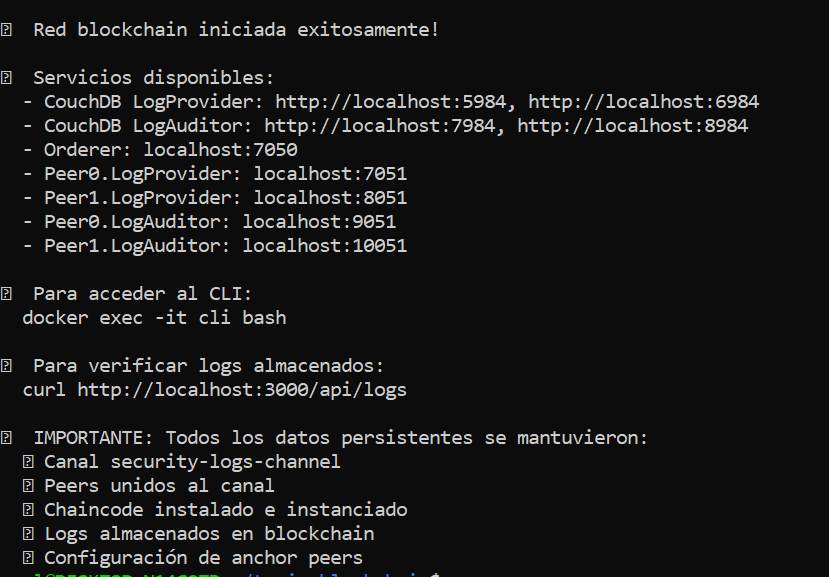
\includegraphics[width=0.8\textwidth]{figuras/script_inicio.png}
    \caption{Ejecución del script de inicialización de la red blockchain}
    \label{fig:script_inicio}
\end{figure}

El script ejecuta una secuencia predefinida de pasos que aseguran la correcta inicialización de cada componente. Esta automatización resultó esencial durante las múltiples iteraciones de prueba del sistema, ya que permite recrear el entorno completo en cuestión de minutos.

\subsection{Verificación de Componentes Activos}
Una vez completado el proceso de inicialización, es crucial verificar que todos los servicios estén operativos. La Fig \ref{fig:docker_ps} muestra el resultado del comando de verificación.
\begin{figure}[H]
    \centering
    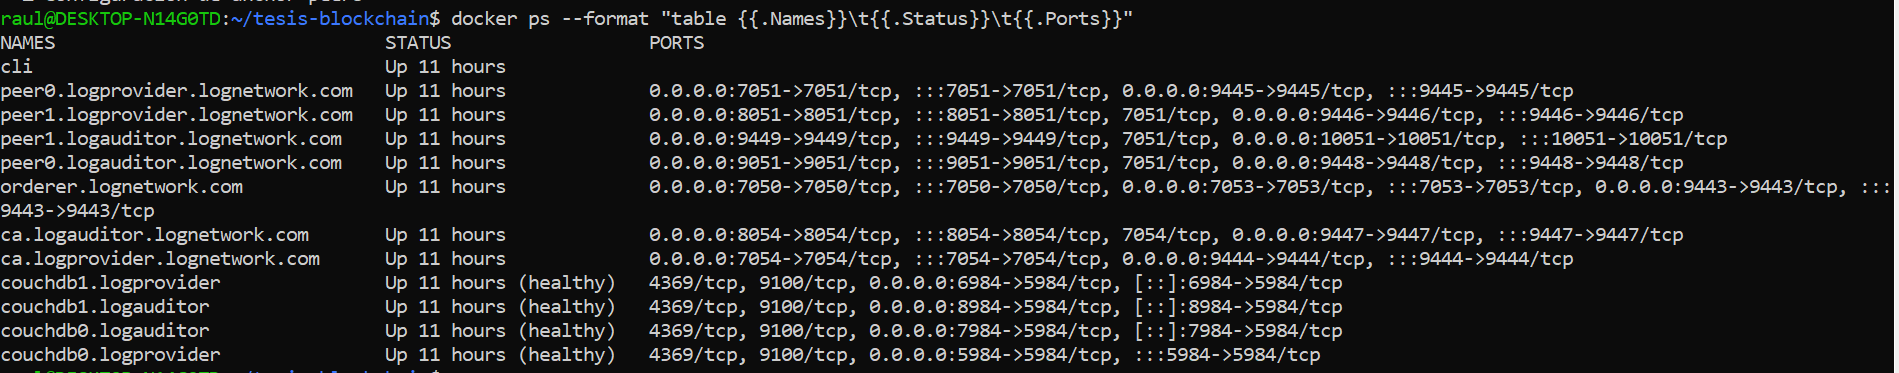
\includegraphics[width=0.9\textwidth]{figuras/docker_ps.png}
    \caption{Contenedores Activos de la Red Blockchain}
    \label{fig:docker_ps}
\end{figure}

Esta verificación confirma que los ocho contenedores principales están ejecutándose correctamente: cuatro nodos peer (dos por organización), un orderer, un CLI, y las instancias de CouchDB correspondientes. El estado “Up” indica que los servicios han superado sus verificaciones de salud internas.

\subsection{Validación del Canal de Comunicación}
Con la infraestructura desplegada, se verifica que el canal security-logs-channel ha sido creado exitosamente. Este canal constituye el espacio compartido donde ambas organizaciones interactúan para el almacenamiento y consulta de logs de seguridad:

Como se observa en la Fig \ref{fig:canal_creado}, el comando \textit{peer channel list} muestra que el canal security-logs-channel está disponible y operativo. Esta confirmación es fundamental ya que establece las políticas de endorsement que requieren la participación de ambas organizaciones para validar cualquier transacción de almacenamiento de logs.
\begin{figure}[H]
    \centering
    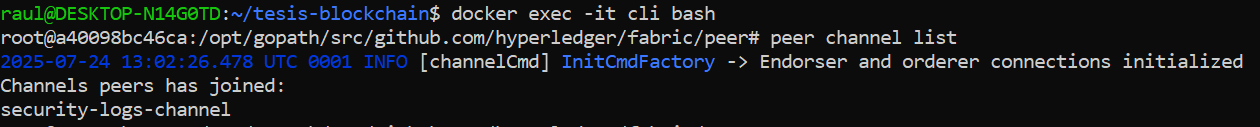
\includegraphics[width=0.8\textwidth]{figuras/canal_creado.png}
    \caption{Verificación de Participación del Peer en el Canal de Seguridad}
    \label{fig:canal_creado}
\end{figure}

\subsection{Captura Automática de Logs del Sistema}
Una vez establecida la infraestructura blockchain, el siguiente componente crítico del sistema es el mecanismo de captura automática de logs de seguridad. Este componente implementa la funcionalidad de interceptar eventos del sistema en tiempo real y determinar cuáles requieren almacenamiento inmutable en la blockchain.
\subsubsection{Inicialización del Collector de Logs}
El sistema de captura se implementó mediante un collector especializado que opera como un servidor UDP, interceptando los logs que el sistema operativo envía a través del protocolo syslog estándar. La inicialización del collector se realiza ejecutando: \textit{node syslog-collector.js}
\begin{figure}[H]
    \centering
    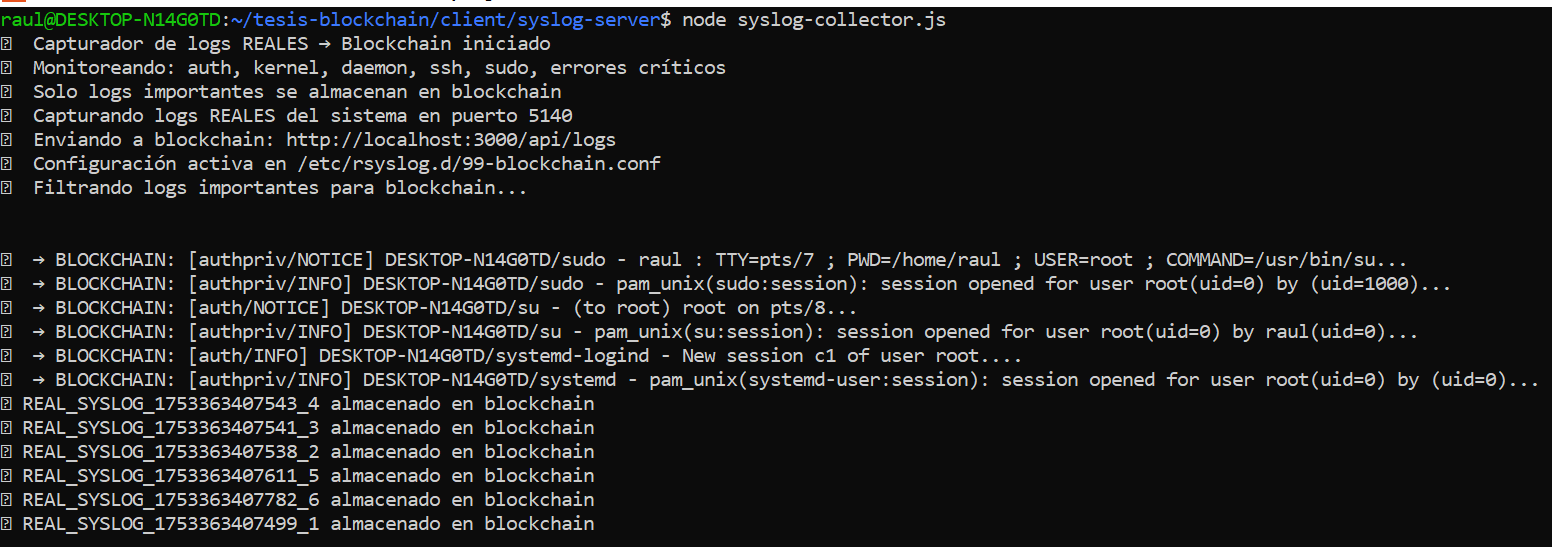
\includegraphics[width=0.8\textwidth]{figuras/collector_inicio.png}
    \caption{Ejecución del Colector de Logs y Almacenamiento en la Blockchain}
    \label{fig:collector_inicio}
\end{figure}

Como se muestra en la Fig \ref{fig:collector_inicio}, el sistema confirma la inicialización exitosa del servidor en el puerto 5140, estableciendo la conectividad con la API blockchain y activando los filtros de logs críticos. Esta configuración permite que el collector reciba automáticamente todos los eventos de seguridad generados por el sistema operativo y las aplicaciones.

\subsubsection{Prueba de Captura Manual}
Para demostrar la capacidad de respuesta del sistema, se ejecutó una prueba de generación manual de logs críticos utilizando la herramienta logger del sistema: \textit{logger -p auth.warning 
“PRUEBA: Intento de acceso no autorizado desde IP 192.168.1.200”}

Como se documenta en la Fig \ref{fig:prueba_manual}, el sistema detecta inmediatamente este evento, lo clasifica como log crítico de seguridad y procede a enviarlo automáticamente a la blockchain. La respuesta es prácticamente instantánea, demostrando la efectividad del mecanismo de captura en tiempo real.
\begin{figure}[H]
    \centering
    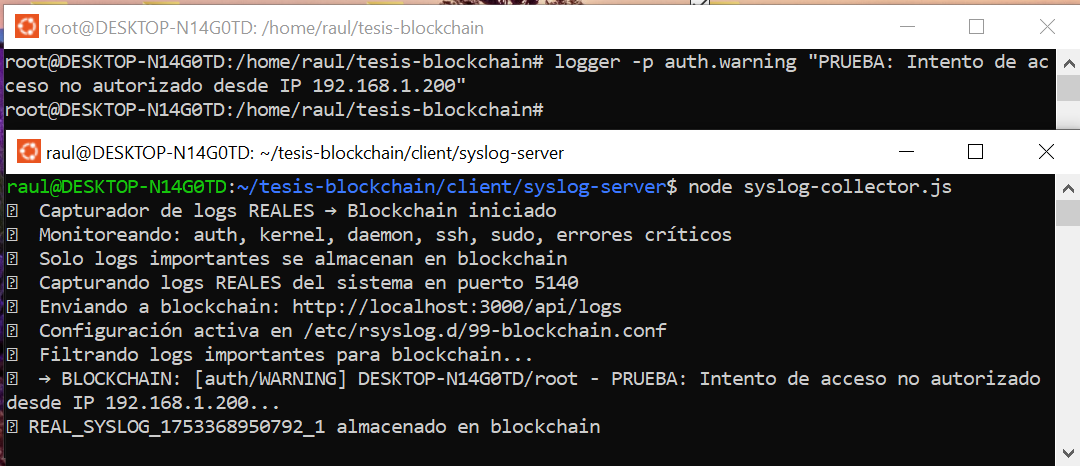
\includegraphics[width=0.8\textwidth]{figuras/prueba_manual.png}
    \caption{Prueba manual de ingreso del log}
    \label{fig:prueba_manual}
\end{figure}

Cada log que cumple los criterios de filtrado se envía automáticamente a la API REST que gestiona la interfaz con la blockchain. El collector confirma la recepción exitosa de cada log, como se muestra en la Fig \ref{fig:confirmacion_envio}, donde se puede observar el identificador único asignado y la confirmación de almacenamiento.
Esta confirmación bidireccional asegura que no se pierdan logs críticos y proporciona trazabilidad completa del proceso de captura y almacenamiento.

\begin{figure}[H]
    \centering
    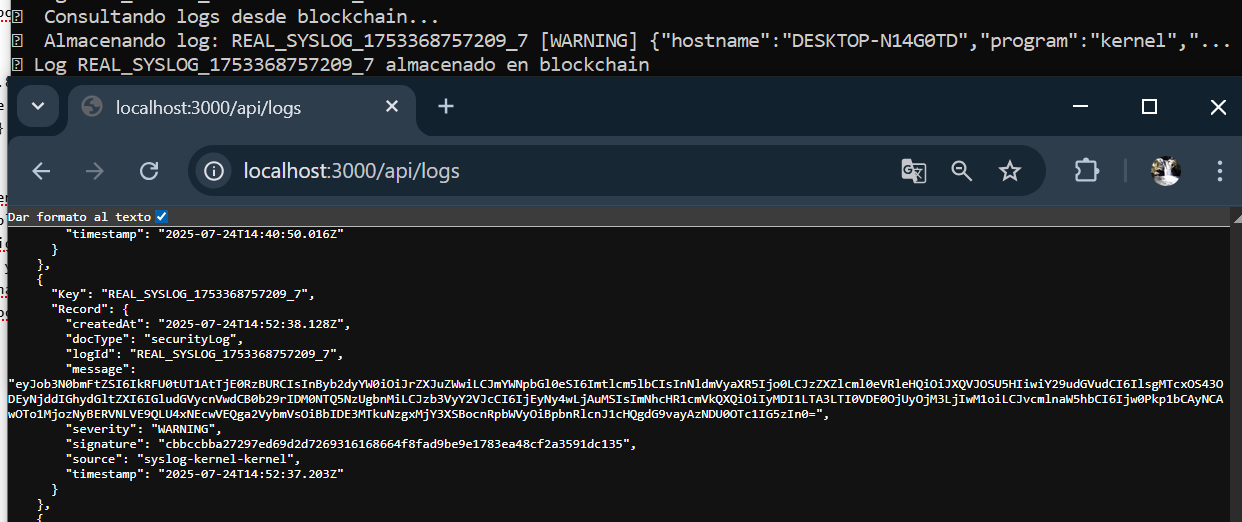
\includegraphics[width=1\textwidth]{figuras/confirmacion_envio.png}
    \caption{Confirmación de envío}
    \label{fig:confirmacion_envio}
\end{figure}

\subsection{Consulta y Verificación de Logs en Blockchain}
La fase final de la demostración del sistema consiste en verificar que los logs capturados y almacenados están efectivamente disponibles en la blockchain y pueden ser consultados a través de múltiples interfaces. Esta verificación confirma la integridad del flujo completo y demuestra las capacidades de auditoría del sistema implementado.
\subsubsection{Verificación Directa via Blockchain}
La forma más directa de verificar el almacenamiento exitoso de logs es consultando directamente la blockchain mediante el CLI de Fabric. Desde el contenedor CLI, se ejecuta \textit{peer chaincode query -C security-logs-channel -n security-logs -c '{“function”:“QuerySecurityLog”,-\\“Args”:[“REAL\_SYSLOG\_1753368757209\_7”]}'}
\begin{figure}[H]
    \centering
    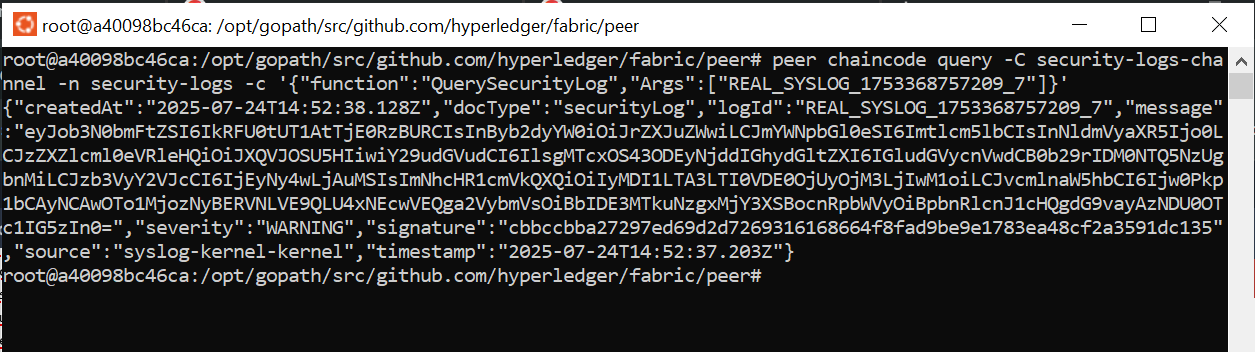
\includegraphics[width=1\textwidth]{figuras/query_blockchain.png}
    \caption{Query dentro de la blockchain}
    \label{fig:query_blockchain}
\end{figure}

Como se muestra en la Fig \ref{fig:query_blockchain}, este comando retorna todos los logs almacenados en formato JSON, incluyendo sus metadatos completos: identificadores únicos, timestamps, niveles de severidad, contenido codificado y firmas hash. Esta consulta directa confirma que los datos están efectivamente persistidos en el ledger distribuido.

\subsubsection{Consulta via API REST}
El sistema también permite la consulta de logs a través de la API REST, proporcionando una interfaz más accesible para aplicaciones externas. La consulta se realiza mediante:\textit{http://localhost:3000/api/logs}
\newpage
\begin{figure}[H]
    \centering
    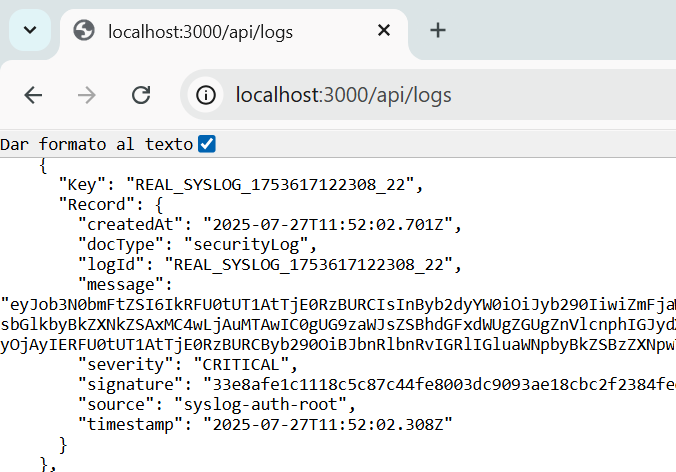
\includegraphics[width=0.8\textwidth]{figuras/api_query.png}
    \caption{Api query para la consulta de logs}
    \label{fig:api_query}
\end{figure}

La Fig \ref{fig:api_query} presenta la respuesta estructurada de la API, que incluye estadísticas del sistema como el conteo total de logs, versión del chaincode activo y timestamp de la consulta. Esta interfaz facilita la integración con sistemas de monitoreo externos y herramientas de análisis forense.


\subsubsection{Dashboard Web Interactivo}
La interfaz web desarrollada proporciona una herramienta integral para la consulta y análisis de logs de seguridad almacenados en blockchain. El dashboard implementa una consulta automáticamente a la red blockchain y presenta la información mediante visualizaciones interactivas.
Como se observa en la Fig \ref{fig:dashboard_principal}, la interfaz se estructura en componentes clave que facilitan el monitoreo de seguridad: un panel de estadísticas en tiempo real que muestra métricas esenciales del sistema , una sección dedicada al último log registrado con información completa del evento más reciente, y gráficos estadísticos que visualizan la distribución por severidad y patrones de actividad temporal.
El sistema incluye funcionalidades adicionales como visualización de logs recientes con capacidad de expansión para análisis detallado, controles de actualización automática, e indicadores de estado de conectividad. 
Esta solución demuestra la viabilidad de integrar tecnología blockchain con interfaces de usuario modernas para crear sistemas de auditoría de seguridad que combinan la inmutabilidad de los datos distribuidos con herramientas de análisis accesibles y funcionales para administradores de sistemas.
\begin{figure}[H]
    \centering
    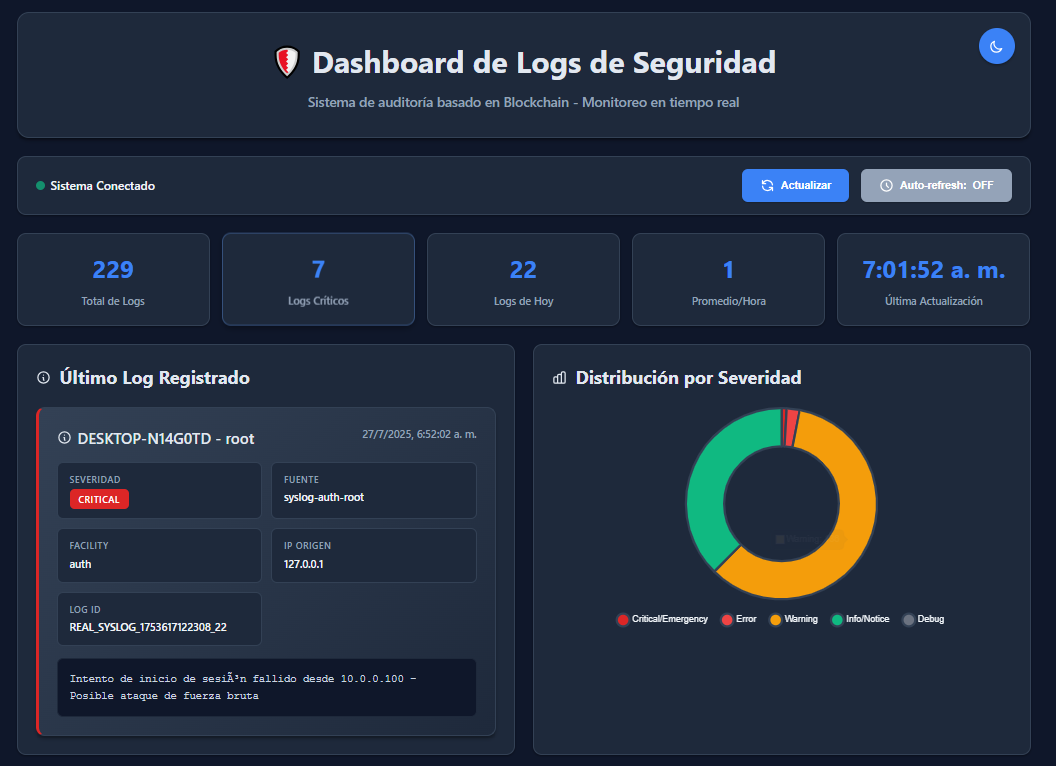
\includegraphics[width=0.8\textwidth]{figuras/dashboard_web.png}
    \caption{Dashboard principal}
    \label{fig:dashboard_principal}
\end{figure}

\subsection{Prueba de inmutabilidad}
Para demostrar la inmutabilidad de los logs de seguridad almacenados en la red blockchain basada en Hyperledger Fabric, se diseñó una prueba práctica que verifica que los logs, una vez registrados, no pueden ser modificados ni eliminados del historial de transacciones. La prueba se realizó en el canal \textit{security-logs-channel}, utilizando el chaincode \textit{security-logs}.

% Creación del log
Primero, se generó un log de seguridad mediante el comando logger, que simuló un evento de seguridad. Este log se almacenó en el ledger utilizando la función \textit{StoreSecurityLog} del chaincode. Para verificar su correcta creación, se consultó el log con el siguiente comando \textit{peer chaincode query -C security-logs-channel -n security-logs -c '{“Args”:[“QuerySecurityLog”,\\“REAL\_SYSLOG\_1753629240230\_92”]}'}

El resultado mostró los detalles del log, incluyendo su logId, timestamp, source, severity, y message, confirmando su almacenamiento en el world state (base de datos CouchDB). La salida de esta consulta se presenta en la Figura~\ref{fig:log-consultado}.

\begin{figure}[H]
    \centering
    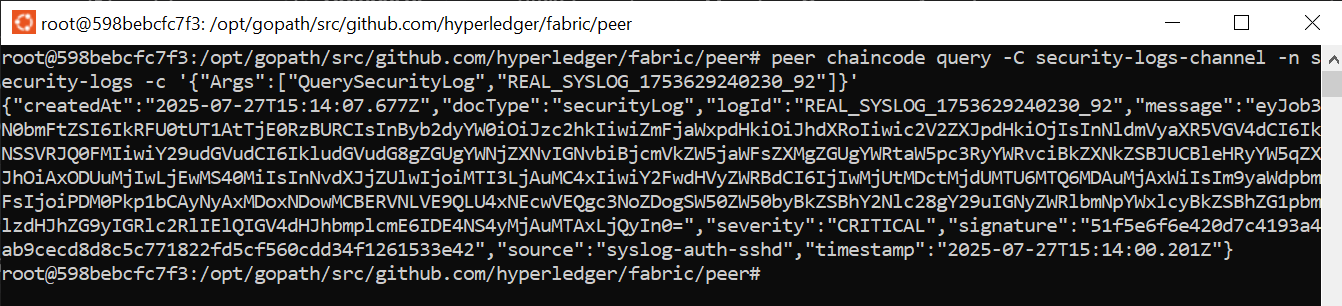
\includegraphics[width=1\textwidth]{figuras/log-consultado.png}
    \caption{Consulta del log REAL\_SYSLOG\_1753629240230\_92 en el world state.}
    \label{fig:log-consultado}
\end{figure}

% Eliminación del log
Posteriormente, se eliminó el log del world state utilizando la función \textit{DeleteSecurityLog} a través del siguiente comando ejecutado desde la interfaz de línea de comandos (CLI),  \textit{peer chaincode invoke -o orderer.lognetwork.com:7050 --tls --cafile /opt/gopath/src/github.com/hyperledger/\\fabric/peer/crypto/ordererOrganizations/lognetwork.com/tlsca/tlsca.lognetwork.com-cert.pem -C \\security-logs-channel -n security-logs -c '{“function”:“DeleteSecurityLog”,“Args”:[“REAL\_\\SYSLOG\_1753629240230\_92”]}'} .

El comando devolvió el mensaje: \textit{Log REAL\_SYSLOG\_1753629240230\_92 deleted successfully}, confirmando la eliminación del log del world state. La salida de esta operación se muestra en la Figura~\ref{fig:log-eliminado}.

\begin{figure}[H]
    \centering
    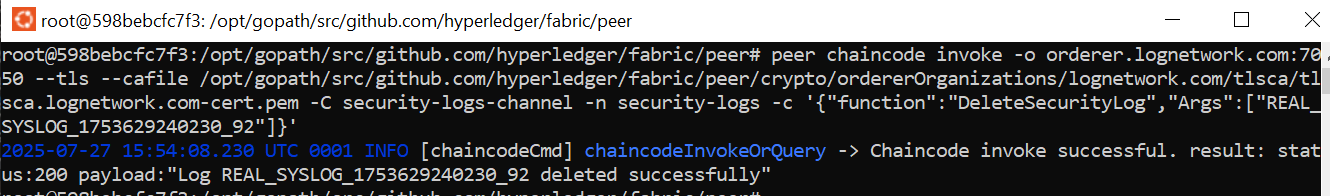
\includegraphics[width=1\textwidth]{figuras/log-eliminado.png}
    \caption{Eliminación del log REAL\_SYSLOG\_1753629240230\_92 del world state.}
    \label{fig:log-eliminado}
\end{figure}

Para confirmar que el log ya no estaba en el world state, se intentó consultarlo nuevamente con \textit{peer chaincode query -C security-logs-channel -n security-logs -c '{“Args”:[“QuerySecurityLog”,\\“REAL\_SYSLOG\_1753629240230\_92”]}'}


El resultado arrojó un error: \textit{Log REAL\_SYSLOG\_1753629240230\_92 does not exist}, verificando que el log fue eliminado del estado actual del ledger.

Para probar la inmutabilidad del log, se examinaron las transacciones almacenadas en el blockchain. Aunque el log fue eliminado del world state, el historial de su creación permanece en el blockchain debido a su naturaleza inmutable. Se consultó el bloque 8 del canal \textit{security-logs-channel} utilizando el chaincode del sistema \textit{qscc} con el siguiente comando, 

\textit{peer chaincode query -C security-logs-channel -n qscc -c '{“Args”:[“GetBlockByNumber”\\,“security-logs-channel”,“8”]}'}

La salida reveló que el log con el identificador \textit{REAL\_SYSLOG\_1753629240230\_92} estaba presente en el \textit{write set} de una transacción en el bloque 8, como se muestra en la Figura~\ref{fig:log-write-set}, confirmando que el historial de su creación no fue alterado. La inmutabilidad se deriva de la estructura del blockchain, donde cada bloque contiene un hash del bloque anterior, asegurando que las transacciones registradas no puedan modificarse sin romper la integridad de la cadena. Esto garantiza que, aunque el log fue eliminado del world state, su registro histórico permanece accesible e inalterable en el blockchain, cumpliendo con el objetivo de trazabilidad e integridad de los logs de seguridad.

\begin{figure}[H]
    \centering
    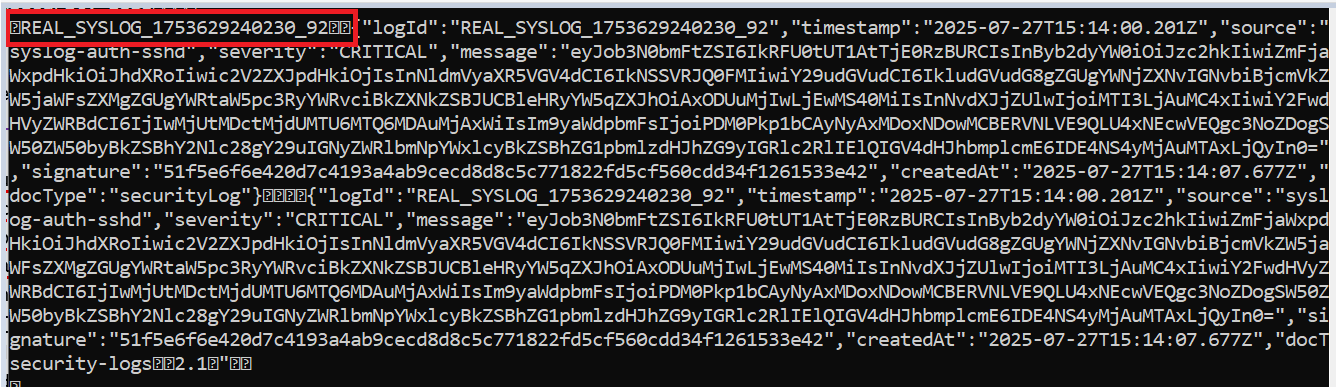
\includegraphics[width=1\textwidth]{figuras/log-write-set.png}
    \caption{Log REAL\_SYSLOG\_1753629240230\_92 en el write set del bloque 8.}
    \label{fig:log-write-set}
\end{figure}
\newpage

\section{Conclusiones y recomendaciones}


\subsection{Conclusiones}

Se desarrolló exitosamente un sistema basado en blockchain que garantiza la integridad, trazabilidad y autenticidad de logs de seguridad, cumpliendo con el objetivo planteado. La solución integra tecnologías emergentes como Hyperledger Fabric, criptografía avanzada y arquitectura distribuida, proporcionando un modelo escalable y replicable para infraestructuras críticas donde la inmutabilidad de los registros es fundamental.

El análisis realizado sobre los métodos convencionales de almacenamiento y gestión de logs de seguridad permitió evidenciar limitaciones significativas en cuanto a la integridad, trazabilidad y autenticidad de los registros. Estos enfoques, al basarse en infraestructuras centralizadas y carentes de mecanismos robustos de verificación, resultan vulnerables a manipulaciones y eliminaciones no autorizadas, comprometiendo así la confiabilidad del sistema ante auditorías o análisis forenses.

La implementación de una red blockchain permisionada con Hyperledger Fabric 2.5 demostró ser una solución técnica viable para garantizar la inmutabilidad y la seguridad de los logs. La configuración de una arquitectura multi-organización, el uso del consenso etcdraft, certificados digitales X.509, canales privados y cifrado TLS en todos los componentes, permitió establecer un entorno distribuido, confiable y resistente a alteraciones maliciosas, alineado con los principios de una gestión segura de registros.

El mecanismo de recolección de logs en tiempo real, implementado mediante servidor rsyslog, logró capturar y procesar logs según el estándar RFC3164. Este componente aplicó filtros inteligentes basados en severidad, programas críticos y palabras clave de seguridad, y evitó duplicaciones mediante el uso de hash MD5.  La implementación de firmas digitales SHA-256 garantizó la integridad de cada registro antes de su inserción en la blockchain.

El smart contract denominado \textit{security-logs}, desarrollado en Node.js, permitió gestionar de forma segura las operaciones de almacenamiento, consulta y eliminación de registros. 

El smart contract "security-logs" desarrollado en Node.js demostró un rendimiento óptimo en las operaciones CRUD. El uso de estructuras JSON serializadas y el manejo de errores robusto garantizaron la consistencia de los datos. La API REST en Express.js facilitó la interacción con el sistema y su integración con aplicaciones externas.

La interfaz expuesta a través de la API REST ofreció una herramienta eficaz para consultar, validar y visualizar los logs almacenados en la blockchain. Esto permitió garantizar el acceso a registros íntegros, no repudiables y completamente trazables, fortaleciendo las capacidades de auditoría y supervisión de los entornos donde fue desplegado el sistema.


\subsection{Recomendaciones}

La incorporación de scripts shell especializados en el despliegue de la red blockchain permite garantizar la consistencia del entorno, minimizar errores humanos y facilitar tareas de mantenimiento y auditoría. Estos scripts deben diseñarse siguiendo una estructura modular basada en responsabilidades únicas, lo que permite una gestión clara de cada fase del proceso: creación de canales, incorporación de nodos y despliegue de smart contracts.

El correcto funcionamiento de una red basada en Hyperledger Fabric depende de una secuencia precisa y validada en la inicialización de sus contenedores. La infraestructura debe levantarse en fases claramente definidas y con verificaciones de estado: primero las bases de datos CouchDB con confirmación de conectividad, seguidas por las autoridades de certificación con generación exitosa de certificados X.509, luego el nodo ordenante (orderer) con configuración del algoritmo de consenso, posteriormente los nodos peer con sincronización del ledger, y finalmente las herramientas administrativas como el CLI.

Para garantizar la sostenibilidad a largo plazo del sistema, es importante implementar una estrategia integral de escalabilidad que considere el crecimiento esperado del volumen de logs y la expansión de la infraestructura monitoreada. Esto incluye la configuración de métricas de rendimiento en tiempo real, establecimiento de umbrales de alerta para transacciones por segundo, utilización de recursos y latencia de consenso.


\subsection{Trabajos futuros}

La evolución inmediata del sistema contempla la expansión de sus capacidades analíticas mediante el desarrollo de un dashboard web avanzado que incorpore técnicas de visualización de datos de última generación. Se proyecta una interfaz intuitiva basada en principios de diseño centrado en el usuario que permita a auditores y administradores de seguridad realizar consultas complejas sin requerir conocimientos especializados en blockchain.

Como estrategia de mediano plazo, se contempla la implementación de una arquitectura multi-nodo geográficamente distribuida que incorpore nodos de diferentes organizaciones bajo un modelo de consorcio. Esta expansión no solo incrementará la disponibilidad y tolerancia a fallos del sistema, sino que permitirá la validación cruzada de logs entre entidades colaboradoras, fortaleciendo la confianza y la integridad de los registros.

Un desarrollo del sistema involucra su integración con plataformas SIEM existentes, sistemas de threat intelligence y frameworks de respuesta a incidentes. Se prevé el desarrollo de conectores estandarizados que permitan la interoperabilidad con soluciones como Splunk, IBM QRadar, y herramientas de código abierto como ELK Stack, facilitando la adopción gradual sin reemplazar completamente las infraestructuras actuales.

Finalmente, se considera la posibilidad de implementar un enfoque multi-cadena, en el que distintos tipos de registros se almacenen en canales o cadenas independientes, aplicando políticas diferenciadas de acceso y control. Esta segmentación optimiza la escalabilidad del sistema y refuerza la confidencialidad de los datos almacenados.

\newpage

% Referencias
\section{Referencias Bibliográficas}
\renewcommand\refname{}
\printbibliography
\newpage

% Anexos
%\input{capitulos/anexos}

\end{document}